% \documentclass[14pt,a4paper]{report}
\documentclass[14pt,a4paper]{article}
\usepackage[utf8]{inputenc}
\usepackage[english,vietnamese]{babel}
\usepackage[left=3.50cm, right=2.00cm, top=2.00cm, bottom=2.00cm]{geometry}
\usepackage{multirow}
\usepackage{listings}
\lstset{basicstyle=\ttfamily,escapechar=\@}
\usepackage{paralist}
\usepackage{graphicx}
\usepackage{wrapfig}
\usepackage{setspace}
\usepackage{amsthm}
\usepackage{array}
\usepackage{hyperref}
\hypersetup{colorlinks=true,pdfencoding=auto}
\usepackage{hypcap}
\usepackage{longtable}
\usepackage{rotating}
\usepackage{subfig}
\usepackage{float}
\renewcommand{\baselinestretch}{1.3}
\usepackage{indentfirst}
\usepackage{pgfgantt}
\usepackage{amsmath}
\usepackage{fancybox}
\usepackage{tabto}
\setcounter{tocdepth}{4}
\setcounter{secnumdepth}{4}
\selectlanguage{vietnamese}

\begin{document}

\newgeometry{top=2cm, bottom=2cm, left=2cm, right=2cm}
\begin{titlepage}
\begin{center}

\vspace*{3\bigskipamount}

\begin{otherlanguage*}{vietnamese}
\makeatletter
\fontsize{12}{12}\textbf{ĐẠI HỌC QUỐC GIA TP HỒ CHÍ MINH}\\
\fontsize{14}{14}\textbf{TRƯỜNG ĐẠI HỌC BÁCH KHOA}\\
\fontsize{14}{14} -----------------------------------
\makeatother
\vspace{3cm}
% \begin{figure}[h]
%     \centering
%     
\includegraphics[width=0.4\columnwidth]{./cover/bk.png}
% \end{figure}

{\makeatletter
\fontsize{16}{16}\textbf{TRẦN HOÀNG TUẤN}\\
\makeatother}
\vspace{3cm}

{\makeatletter
\fontsize{16}{16}\textbf{SINH BIỂU CẢM KHUÔN MẶT DỰA TRÊN PHÙ HỢP GIỌNG NÓI}\\
\vspace{1cm}
\fontsize{12}{12} CHUYÊN NGÀNH: KHOA HỌC MÁY TÍNH\\
\fontsize{12}{12} MÃ SỐ: 8480101\\
\makeatother}

\vspace{1.2cm}
{\makeatletter
\fontsize{18}{18}\textbf{LUẬN VĂN THẠC SĨ}\\
\makeatother}


\vspace{8cm}
{\makeatletter
\fontsize{12}{12} TP.HỒ CHÍ MINH, tháng 07 năm 2021\\
\makeatother}

\end{otherlanguage*}

\end{center}
\end{titlepage}

\restoregeometry

\begin{titlepage}
\begin{center}

\vspace*{3\bigskipamount}

\begin{otherlanguage*}{vietnamese}
\makeatletter
\fontsize{12}{12}\textbf{ĐẠI HỌC QUỐC GIA TP HỒ CHÍ MINH}\\
\fontsize{14}{14}\textbf{TRƯỜNG ĐẠI HỌC BÁCH KHOA}\\
\fontsize{14}{14} -----------------------------------
\makeatother
\vspace{3cm}
% \begin{figure}[h]
%     \centering
%     
\includegraphics[width=0.4\columnwidth]{./cover/bk.png}
% \end{figure}

{\makeatletter
\fontsize{16}{16}\textbf{TRẦN HOÀNG TUẤN}\\
\makeatother}
\vspace{3cm}

{\makeatletter
\fontsize{16}{16}\textbf{SINH BIỂU CẢM KHUÔN MẶT DỰA TRÊN PHÙ HỢP GIỌNG NÓI}\\
\vspace{1cm}
\fontsize{12}{12} CHUYÊN NGÀNH: KHOA HỌC MÁY TÍNH\\
\fontsize{12}{12} MÃ SỐ: 8480101\\
\makeatother}

\vspace{1.2cm}
{\makeatletter
\fontsize{18}{18}\textbf{LUẬN VĂN THẠC SĨ}\\
\makeatother}


\vspace{8cm}
{\makeatletter
\fontsize{12}{12} TP.HỒ CHÍ MINH, tháng 07 năm 2021\\
\makeatother}

\end{otherlanguage*}

\end{center}
\end{titlepage}

\begin{titlepage}
\begin{otherlanguage*}{vietnamese}

    \begin{minipage}[t]{0.42\textwidth}
        \begin{center}
            ĐẠI HỌC QUỐC GIA TPHCM\\
            \textbf{TRƯỜNG ĐẠI HỌC BÁCH KHOA}\\
            \textbf{---------------------------}\\
        \end{center}
    \end{minipage}
    \noindent
    \begin{minipage}[t]{0.57\textwidth}
        \begin{center}
            \textbf{CỘNG HÒA XÃ HỘI CHỦ NGHĨA VIỆT NAM}\\
            \textbf{Độc lập - Tự do - Hạnh phúc}\\
            \textbf{---------------------------}\\
        \end{center}
    \end{minipage}

    \begin{center}
        \fontsize{18}{18}\textbf{NHIỆM VỤ LUẬN VĂN THẠC SĨ}
    \end{center}

    \begin{flushleft}
        Họ tên học viên: Trần Hoàng Tuấn
        \tabto{10cm}
        MSHV: 1970220\\
        Ngày, tháng, năm sinh: 01/08/1996
        \tabto{10cm}
        Nơi sinh: Đồng Nai\\
        Chuyên ngành: Khoa học dữ liệu
        \tabto{10cm}
        Mã số:\\

        \renewcommand{\labelenumi}{\Roman{enumi}}
        \begin{enumerate}
            \item \textbf{TÊN ĐỀ TÀI: SINH BIỂU CẢM KHUÔN MẶT DỰA TRÊN PHÙ HỢP GIỌNG NÓI}
            \item \textbf{NHIỆM VỤ VÀ NỘI DUNG:}
            \item \textbf{NGÀY GIAO NHIỆM VỤ:}
            \item \textbf{NGÀY HOÀN THÀNH NHIỆM VỤ:}
            \item \textbf{CÁN BỘ HƯỚNG DẪN:}
        \end{enumerate}
    \end{flushleft}

    \begin{flushright}
        \textit{Tp.HCM, ngày .... tháng .... năm 2021}
    \end{flushright}

    \begin{center}
        \begin{minipage}[t]{0.45\textwidth}
            \center\textbf{CÁN BỘ HƯỚNG DẪN}\\
            (Họ tên và chữ ký)
            \vspace{3cm}
        \end{minipage}
        \noindent
        \begin{minipage}[t]{0.45\textwidth}
            \center\textbf{CHỦ NHIỆM BỘ MÔN ĐÀO TẠO}\\
            (Họ tên và chữ ký)
            \vspace{3cm}
        \end{minipage}
        \begin{minipage}[t]{0.90\textwidth}
            \center\textbf{TRƯỞNG KHOA}\\
            (Họ tên và chữ ký)
            \vspace{3cm}
        \end{minipage}
    \end{center}

\end{otherlanguage*}
\vfill
\end{titlepage}

\begin{titlepage}
\begin{otherlanguage*}{vietnamese}

\begin{center}
    \fontsize{18}{18}\textbf{LỜI CẢM ƠN}
\end{center}

\end{otherlanguage*}
\vfill
\end{titlepage}
\thispagestyle{plain}
\chapter*{\centering \begin{huge}Abstract\end{huge}}

\noindent
%\large
\textit{Speech-driven facial animation} is a hot research topic in recent years since it has many applications in our real life. The aim of this problem is to generate videos that synthesize a talking face of an arbitrary person based on speech audio. It also comes with many challenges. The synthesized videos are considered high quality when the shape of mouth has high correlation with the given speech, the human face in video should be created as real as possible and identity of the person should be kept. This research proposes a method to generate facial animation from speech. Our approach inherits from this paper \cite{chen2019}, we also use the facial landmark normalization method from the paper \cite{gen_face_landmark} to improve video quality. In the paper \cite{chen2019}, they design a cascade deep learning system to effectively synthesize talking face video. This method uses a neural network to convert speech audio to a facial landmark sequence that describes face movement. In the end, they use a GANs network to generate video based on the landmark sequence that has just been created in the last step. At the step of creating a landmark sequence, we apply the normalization method from \cite{gen_face_landmark} with some modification so that it can be fitted to our system. It helps our system to create more realistic and high quality videos. All experiments in this thesis are performed on these two datasets: GRID \cite{grid} and LRW \cite{lrw}. The result shows that our approach creates videos with higher quality than the baseline method.

\clearpage
\begin{titlepage}
\begin{otherlanguage*}{vietnamese}

\begin{center}
    \fontsize{18}{18}\textbf{LỜI CAM ĐOAN}
\end{center}

Tôi là Trần Hoàng Tuấn, học viên cao học khoa Khoa Học và Kỹ thuật Máy Tính, đại học Bách Khoa TP.HCM, MSHV là 1970220. Tôi xin cam đoan luận văn \textbf{"SINH BIỂU CẢM KHUÔN MẶT DỰA TRÊN PHÙ HỢP GIỌNG NÓI"} là công trình nghiên cứu của riêng tôi dưới sự hướng dẫn khoa học của TS. Nguyễn Quang Hùng. Các số liệu trong luận văn được sử dụng trung thực, kết quả nghiên cứu trong luận văn này chưa từng được công bô tại bất kì công trình nào khác. Các công trình, bài báo tham khảo trong luận văn đều được trích dẫn đầy đủ. Các công cụ được sử dụng trong luận văn đều là mã nguồn mở và không vi phạm luật bản quyền.

\begin{flushright}
    \begin{minipage}[t]{0.50\textwidth}
    \begin{center}
        TPHCM, ngày 05 tháng 08 năm 2021\\
        Tác giả luận văn\\
        \vspace{3cm}
        \textbf{Trần Hoàng Tuấn}
    \end{center}
    \end{minipage}
\end{flushright}


\end{otherlanguage*}
\vfill
\end{titlepage}

\pagenumbering{gobble}
\tableofcontents
\listoffigures

\pagenumbering{arabic}

\section{\texorpdfstring{Tóm tắt luận văn}{brief}}
% Trình bày ngắn gọn về cấu trúc của Luận văn, giới thiệu những điểm nhấn của Luận văn, kết quả, và các từ khóa đi kèm.

\section{\texorpdfstring{Mở đầu}{open}}
% Nêu lý do chọn đề tài, mục đích, đối tượng và phạm vi nghiên cứu, ý nghĩa khoa học và ý nghĩa thực tiễn của đề tài.

Trong những năm gần đây, với sự bùng nổ và phát triển cực kì mạnh mẽ của ngành công nghệ thông tin và đặc biệt là ngành trí tuệ nhân tạo, ngày càng nhiều các sáng kiến đôc đáo đã được sinh ra. Trong đó, việc tạo sinh dữ liệu tự động sử dụng trí tuệ nhân tạo đã đánh dấu một bước chuyển mình mới và cực kì sáng tạo.

So với các mô hình truyền thống với mục đích phân lớp, phân đoạn, gom nhóm, và dự đoán theo chuỗi thời gian, nhóm các mô hình tạo sinh dữ liệu được sinh ra với mục đích hoàn toàn khác. Trong khi các mô hình truyền thống cung cấp thông tin đã hiện hữu trong thế giới thực (bài toán nhận diện vật thể, OCR, phân đoạn hình ảnh,...) hoặc các dự đoán về các sự kiện sẽ xảy ra (dự đoán giá chứng khoán, dự đoán diễn biến dịch COVID-19,...), thì các mô hình tạo sinh dữ liệu lại cố gắng tạo ra dữ liệu mới, chưa từng tồn tại trong thế giới thực.

Một số ví dụ về việc tạo sinh dữ liệu bằng trí tuệ có thể kể đến như: sử dụng mạng LSTM để sáng tác nhạc, hay công trình chuyển đổi phong cách hình ảnh (style transfer) của giáo sư Fei Fei Li và cộng sự \cite{Johnson2016Perceptual}, hay trang web \url{https://thispersondoesnotexist.com}, được tạo nên để tạo sinh những gương mặt người chưa từng tồn tại bằng mạng StyleGAN2 \cite{stylegans}.

Bài toán tạo sinh dữ liệu dựa trên những nguồn dữ liệu có tính chất khác nhau đã và đang trở thành xu thế trong những năm trở lại đây. Đây là bài toán có tính cấp bách, mang lại giá trị cao về mặt kiến thức cho ngành trí tuệ nhân tạo nói riêng và giá trị về mặt kinh tế, công nghệ chung cho toàn xã hội xã hội. Bên cạnh đó, việc tạo sinh dữ liệu về con người đã đạt được những tiến bộ vượt bậc, đặc biệt là tạo sinh dữ liệu hình ảnh khuôn mặt người.

Kiến trúc mạng Generative Adversarial Network \cite{gans_base} ra đời vào năm 2014 đã đánh dấu một bước chuyển mình mới cho ngành trí tuệ nhân tạo. Kiến trúc này giúp cho việc tạo sinh dữ liệu được thực hiện một cách hiệu quả và chính xác hơn. Dựa trên nền tảng đó, các nghiên cứu về việc tạo sinh ảnh gương mặt người cũng được tiến hành và ngày càng có những bước tiến mới.

\subsection{\texorpdfstring{Lý do chọn đề tài}{Why}}
Việc tạo sinh hình ảnh khuôn mặt người dựa trên tiếng nói đang là nhu cầu cần thiết trong ngành giải trí, phim ảnh, hoạt hình. Nếu xây dựng được một hệ thống tạo hình khuôn mặt tốt, chi phí sản xuất phim sẽ được giảm thiểu đáng kể vì phần hóa trang có thể được cắt bớt, phần kĩ xảo có thể được đơn giản hóa, diễn viên không phải quá mạo hiểm trong các cảnh quay nguy hiểm. Đối với hoạt hình, phần hình vẽ có thể được hỗ trợ rất nhiều bởi hệ thống tạo sinh khuôn mặt, từ đó có thể giảm bớt chi phí vẽ hình. Bên cạnh đó, ta có thể tạo sinh gương mặt đại diện trong trường hợp người nói không muốn lộ diện. Ngoài những ứng dụng rất hữu ích trong thực tiễn như đã nêu ở trên, bài toán tạo sinh gương mặt còn là một bài toán khó, thú vị và mới mẻ, còn nhiều hướng đi chưa được khai phá và cực kì tiềm năng trong tương lai.

\subsection{\texorpdfstring{Mục đích của nghiên cứu}{Target}}
Nghiên cứu nhằm mục đích kiểm nghiệm các mô hình được đề xuất trong các nghiên cứu gần đây, tìm hiểu các phương pháp tiền xử lý dữ liệu và trích xuất đặc trưng mới giúp mô hình dễ học hơn, tạo sinh ra hình ảnh chân thật và có độ chính xác cao, khó bị nhận biết bởi con người.

\subsection{\texorpdfstring{Đối tượng nghiên cứu}{Objective}}
Đối tượng nghiên cứu của Luận văn là các cách tiếp cận, các phương pháp mô hình hóa bài toán, các mạng học máy, học sâu, mạng GANs và các phương pháp tạo sinh dữ liệu từ mạng GANs, các cấu trúc Residual Encoder-Decoder, bên cạnh đó là các phương pháp kết hợp đặc trưng hình ảnh, âm thanh có xem xét đến thứ tự thời gian để tạo sinh hình ảnh mới.

\subsection{\texorpdfstring{Phạm vi nghiên cứu}{Research}}
Phạm vi nghiên cứu của Luận văn là tạo sinh ảnh giới hạn trong vùng mặt của người, dữ liệu mẫu được cung cấp ban đầu phải là ảnh rõ ràng của khuôn mặt người, đoạn âm thanh được cung cấp cũng phải là âm thanh rõ ràng của tiếng nói.

\subsection{\texorpdfstring{Ý nghĩa khoa học}{ScientificMeaning}}
Đóng góp cho sự phát triển chung của xu hướng tạo sinh dữ liệu mới dựa trên các tính chất của dữ liệu ban đầu. Việc tìm ra phương pháp giải quyết tốt bài toán sẽ tạo nên tảng để giải quyết những bài toán xa hơn, phức tạp hơn như: tạo sinh nửa người trên, tạo sinh toàn bộ cơ thể người, hay tạo sinh cả một bối cảnh trong phim. Đề tài giúp kiểm chứng, hiện thực, thử nghiệm các phương pháp hiện có trong các bài nghiên cứu gần đây, so sánh và tổng hợp để cố gắng tìm ra hướng đi mới, đóng góp thêm phương pháp mới cho việc tạo sinh ảnh. Đồng thời, các phương pháp tạo sinh dữ liệu cũng giúp làm giàu dữ liệu để huấn luyện, kiểm thử cho các mô hình học máy, học sâu khác.

\subsection{\texorpdfstring{Ý nghĩa thực tiễn}{RealLifeMeaning}}
Giải quyết thành công vấn đề này đem lại giá trị to lớn về mặt công nghệ, kinh tế và xã hội. Chúng ta có thể tái hiện lại gương mặt người đang nói ở nhiều thứ tiếng khác nhau, tạo sinh khuôn mặt người đại diện trong các hội nghị trực tuyến, tích hợp vào các trò chơi điện tử để làm chúng trở nên chân thực hơn, truyền video trong điều kiện băng thông giới hạn, giả lập trợ lý ảo có hình dáng con người,... Đối với ngành truyền thông, nó có thể tạo ra biên tập viên ảo. Đối với ngành điện ảnh, giải trí, sáng tạo nội dung nó cũng có giá trị ứng dụng khi giúp giảm bớt áp lực lên khâu hóa trang, kỹ xảo.

\section{\texorpdfstring{Tổng quan tình hình nghiên cứu}{overview}}
% Sơ lược, phân tích, đánh giá các công trình nghiên cứu nổi tiếng có liên quan đến đề tài. Nêu những vấn đề bức thiết cần phải giải quyết, chỉ ra những thiếu sót mà những nghiên cứu trước đây chưa giải quyết được.
Để tạo sinh mặt người đang nói, các công trình nghiên cứu tập trung chủ yếu vào vùng miệng. Bài nghiên cứu vào năm 2018 của Lele Chen \cite{chen2018} đưa ra phương pháp tạo sinh video vùng miệng của người đang nói với đầu vào là ảnh tĩnh của khuôn miệng và một đoạn âm thanh có chứa tiếng nói. Vào năm 2019, Lele Chen \cite{chen2019} và Vougioukas \cite{vougioukas2019} tiếp tục đưa ra phương pháp tạo sinh cả khuôn mặt người dựa vào ảnh tĩnh của khuôn mặt và đoạn âm thanh chứa tiếng nói. Năm 2020, Vougioukas \cite{vougioukas2020} đã cải tiến phương pháp tạo sinh mặt và cập nhật thêm hành động chớp mắt, Lele Chen \cite{chen2020} cũng đưa ra phương pháp mới để tạo sinh mặt hiệu quả hơn, tự nhiên hơn với việc di chuyển của vùng đầu trên khung hình.

Nhìn chung, các nghiên cứu này đã đưa ra các kiến trúc mạng hiệu quả để tạo sinh khuôn mặt cũng như các phương pháp, lập luận và chứng minh tính hiệu quả của các kiến trúc mạng được đề xuất. Mặc dù các thông số của thử nghiệm đưa ra là khá tốt, các nghiên cứu của Vougioukas vẫn chưa thể tạo ra chuyển động của đầu, kết quả tạo sinh của Vougioukas đôi khi không giữ được đặc trưng của ảnh. Nghiên cứu của Lele Chen năm 2020 \cite{chen2020} đã tạo ra chuyển động cho phần đầu dựa trên tiếng nói, nhưng khuôn mặt được tạo sinh vẫn còn có thể bị nhận ra qua các phép thử Turing, và chuyển động của đầu đôi khi vẫn chưa được tự nhiên, mạng cũng có cấu trúc rất phức tạp và đòi hỏi nhiều tài nguyên tính toán để có thể huấn luyện.

\section{\texorpdfstring{Mục tiêu và nhiệm vụ nghiên cứu}{target_and_mission}}
%Mục tiêu và nhiệm vụ nghiên cứu

\subsection{\texorpdfstring{Mục tiêu}{Target}}
Mục tiêu của Luận văn Tốt nghiệp là nghiên cứu các đề tài có liên quan bằng cách khảo sát, kiểm định và thử nghiệm các nghiên cứu mới nhất hiện có, qua đó tiến hành các thử nghiệm để đưa ra một mô hình tạo sinh mặt người đang nói có độ chính xác cao và chân thật. Hình ảnh được tạo ra phải sắc nét, ít nhiễu và tương đồng về mặt nhận dạng, cấu trúc với hình ảnh người mẫu. Đồng thời, khẩu hình miệng của hình ảnh được tạo ra phải khớp với tiếng nói, phù hợp với cách phát âm từ ngữ. Bên cạnh đó, video được tạo ra phải có tính liền lạc, ổn định, không bị hiện tượng nhảy hình. Mục tiêu được đặt ra nhằm thử nghiệm các mô hình hiện có, tăng tính ứng dụng của việc tạo sinh mặt người vào thực tiễn cuộc sống.

\section{\texorpdfstring{Cơ sở lý thuyết}{base_knowledge}}
%Trình bày cơ sở lý thuyết, các lập luận, căn cứ khoa học được sử dụng trong Luận văn.

\subsection{\texorpdfstring{Trí tuệ nhân tạo, học máy và học sâu}{ai_ml_dl}}

Định nghĩa:
\begin{itemize}
    \item \textbf{Trí tuệ nhân tạo:} Là ngành nghiên cứu về cách thực hiện các chương trình máy tính có khả năng mô phỏng suy nghĩ và khả năng giải quyết vấn đề ở cấp độ con người
    \item \textbf{Học máy:} Là tập con của ngành trí tuệ nhân tạo, là ngành nghiên cứu cách thực hiện các chương trình máy tính mà không phải có mã lập trình tường minh, có chức năng tự động học các tri thức của con người để cải thiện các quyết định của nó trên các dữ liệu mà nó chưa từng gặp trước đây.
    \item \textbf{Học sâu:} Là tập con của ngành học máy, là tập hợp các giải thuật học máy có sử dụng mạng thần kinh nhân tạo có cấu trúc tương tự mạng thần kinh trong não bộ con người để học cách đưa ra quyết định.
\end{itemize}

\begin{figure}[H]
    \centering
    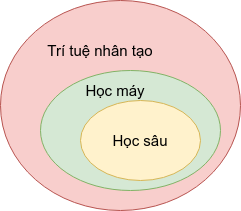
\includegraphics[width=7cm]{./content/materials/ai_ml_dl.png}
    \caption{Trí tuệ nhân tạo, học máy và học sâu}
\end{figure}


Ngày nay, ngành học máy và học sâu ngày càng chiếm nhiều ưu thế so với các phương pháp khác trong các ứng dụng thực tế do có độ tổng quát dữ liệu tốt, độ chính xác cao, và có thể mô hình hóa các vấn đề phức tạp, trừu tượng trong đời sống. Đối với các vấn đề phức tạp như thị giác máy, dịch máy, đánh nhãn văn bản tự động, tạo sinh dữ liệu,... các giải thuật học sâu luôn là lựa chọn hoàn hảo do nó có khả năng tổng quát hóa một lượng dữ liệu rất lớn. Một lợi điểm khác của việc sử dụng các giải thuật học sâu là các giải thuật này có khả năng tìm ra các đặc trưng của dữ liệu một cách tự động. Trong khi các giải thuật học máy truyền thống chỉ có khả năng xử lý tốt trên dữ liệu đã được rút trích đặc trưng bằng các giải thuật xử lý dữ liệu truyền thống, các mạng học sâu có khả năng tự học lấy các đặc trưng của dữ liệu. Tuy nhiên, các giải thuật học sâu yêu cầu một lượng dữ liệu lớn để học. Bên cạnh đó, bài toán phải được mô hình hóa hợp lý, mạng thần kinh học sâu cũng phải được thiết kế phù hợp với mô hình bài toán để khiến cho việc học của mạng thần kinh dễ dàng và hiệu quả hơn.

\subsection{\texorpdfstring{Tính chất tổng quát hóa dữ liệu của mạng thần kinh học sâu}{dl_network}}
Mạng thần kinh học sâu có khả năng tổng quát hóa dữ liệu cao, nhờ vào đó, nó có thể được huấn luyện để học bất cứ thứ gì nếu nó được mô hình hóa một cách hợp lý. Một mạng học sâu đạt được mức độ tổng quát hóa dữ liệu cao bằng cách học những đặc trưng ẩn của dữ liệu được dùng để huấn luyện nó. Vì vậy, mạng học sâu có thể đưa ra dự đoán trên những dữ liệu mới mà nó chưa từng nhìn thấy nhờ vào việc nội suy, nhưng những dữ liệu đó phải tương tự với dữ liệu được dùng để huấn luyện nó. Với những dữ liệu nằm ngoài phân phối dữ liệu huấn luyện, mạng thần kinh học sâu sẽ không có khả năng đưa ra kết quả chính xác bởi cấu trúc và các thông số trong mạng thần kinh không được điều chỉnh đề phù hợp với những dữ liệu đó.

\subsection{\texorpdfstring{Các cấu trúc trong mạng học sâu được sử dụng trong luận văn}{dl_basic_structures}}

\subsubsection{Mạng thần kinh tích chập (Convolution)}
Trước khi có mạng học sâu, việc trích xuất đặc trưng bằng các kĩ thuật đặc biệt cho từng loại dữ liệu khác nhau là công đoạn quan trọng nhất trong quá trình giải quyết một bài toán. Lý do là bởi mạng thần kinh truyền thống không có khả năng tạo ra các chiều không gian đủ rộng để tự học các đặc trưng của dữ liệu. Thông thường, phép tích chập được thực hiện bằng các nhân tích chập (kernel). Một phép tích chập được đặc trưng bởi số lượng kênh đầu vào, số lượng kênh đầu ra và kích thước của nhân tích chập.

\begin{figure}[H]
    \centering
    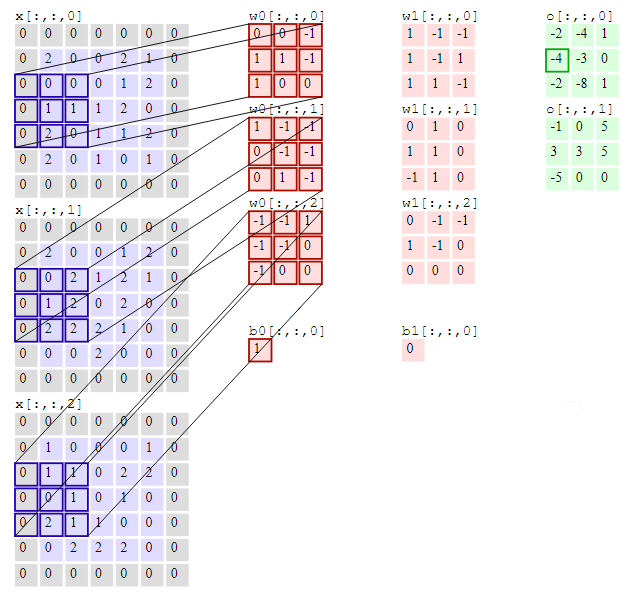
\includegraphics[width=15cm]{./content/materials/cnn.png}
    \caption{Cách tính tích chập. Nguồn: Internet}
\end{figure}

Ví dụ, một phép tích chập với nhân có kích thước $m$x$m$ được thực hiện trên một ma trận ba chiều kích thước $H$x$H$x$K$ sẽ cho ta một ma trận kết quả có kích thước $(N-m+1)$x$(N-m+1)$
Phép tích chập cho ma trận hai chiều trong mạng được biểu diễn bởi phương trình sau:

\begin{equation}
    o_{ijm}=\sum_{k=0}^{K-1}\sum_{p=0}^{H-1}\sum_{q=0}^{H-1}x_{i+p,j+q,k}^{(l-1)}w_{pqkm}+b_{ijm}
\end{equation}

Sự xuất hiện của mạng thần kinh tích chập đã giúp cho việc trích xuất đặc trưng trở nên dễ dàng hơn và đôi khi là không cần thiết nhờ vào khả năng tự động trích xuất đặc trưng của mạng. Sở dĩ mạng thần kinh tích chập có khả năng trích xuất đặc trưng tốt là nhờ vào việc nó tập trung vào học các kiễu mẫu rất chi tiết hay xuất hiện trong dữ liệu ở các lớp đầu. Ở các lớp sau, những tri thức học được càng được tổng quát dần bằng việc kết hợp các tri thức học được từ lớp trước vào tạo nên những hiểu biết ở bậc cao nhất của dữ liệu ở các lớp tích chập cuối cùng.

Nhưng điều này không có nghĩa là chỉ cần sử dụng mạng thần kinh tích chập thì ta sẽ không cần quan tâm tới việc trích xuất đặc trưng nữa bởi khi có những đặc trưng tốt được đưa vào mạng, mạng tích chập vẫn cho ra kết quả tốt hơn, chính xác hơn với ít dữ liệu hơn và thời gian huấn luyện cũng nhanh hơn. Ngoài ra, lớp tích chập cũng có số lượng hệ số học nhỏ, huấn luyện nhanh, vì vậy nó hay được đặt nằm ở các lớp đầu và giữa trong các mạng học sâu để trích xuất dữ liệu nhanh và hiệu quả hơn.

\subsubsection{Tích chập ngược (Deconvolution)}

Đây là mạng có tính năng ngược với mạng tích chập đã được nêu ở phần trên. Nếu như mạng tích chập có chức năng mã hóa, rút trích đặc trưng của dữ liệu đầu vào, thì mạng tích chập ngược nhận vào những đặc trưng đã được rút trích của dữ liệu và tạo sinh ngược lại dữ liệu với cấu trức tương tự ban đầu. Phép tích chập ngược cũng được đặc trưng bởi kích thước nhân, số lượng kênh đầu vào và đầu ra.

Phép tích chập ngược thường hay được sử dụng để tái thiết lập lại cấu trúc ban đầu. Thay vì rút trích và thu nhỏ dữ liệu ban đầu thành những đặc trưng như mạng tích chập, mạng tích chập ngược sử dụng các đặc trưng đã được rút trích và học các trọng số để tạo ra dữ liệu mới có cấu trúc giống với dữ liệu được trích xuất đặc trưng ban đầu. Vì vậy, mạng tích chập ngược có tính năng tạo sin dữ liệu và hay được sử dụng trong các ứng dụng như:

\begin{itemize}
    \item \textbf{Autoencoder:} Một mạng tích chập thu nhỏ và rút trích đặc trưng từ dữ liệu gốc, mạng tích chập ngược dùng véc tơ đặc trưng để cố gắng tái tạo lại dữ liệu gốc.
    \item \textbf{Bài toán phân đoạn ảnh:} Đánh nhãn cho từng điểm ảnh để xem nó thuộc vào lớp nào. Sau khi rút trích đặc trưng từ ảnh, mạng tích chập ngược được dùng để biên dịch đặc trưng ảnh thành mặt nạ phân lớp cho ảnh.
    \item \textbf{Variational Autoencoder:} Một loại mạng nơ ron dùng để tạo sinh dữ liệu dựa trên phân phối xác suất mà nó học được từ dữ liệu mẫu. Với phân phối xác suất học được, mạng có thể tạo ra được dữ liệu có tính chất, cấu trúc tương tự như dữ liệu mẫu nhưng chưa từng tồn tại trong dữ liệu mẫu. Ví dụ: cho mạng Variational Autoencoder học cách tạo sinh hình ảnh của các chữ số trong tập MNIST, sau đây là ảnh được tạo sinh: 
        \begin{figure}[H]
            \centering
            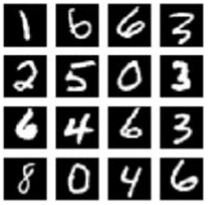
\includegraphics[width=7cm]{./content/materials/mnist_vae.png}
            \caption{Tạo sinh ảnh cùng phân phối xác suất với tập dữ liệu MNIST}
        \end{figure}
    \item \textbf{Mạng GANs (Generative Adversarial Networks):} Là một loại mạng tạo sinh dữ liệu bằng cách học cấu trúc dữ liệu của các mẫu được dùng để huấn luyện, và cũng là cấu trúc mạng được dùng trong luận văn.
\end{itemize}

\subsubsection{Lớp kết nối đầy đủ (Fully Connected)}
Lớp kết nối đầy đủ là lớp chính của mạng nơ ron truyền thống và được xem là một phép biến đổi tuyến tính trong mạng học sâu với phương trình:
\begin{equation}
    y=xA^T+b
\end{equation}
Với phương trình trên, lớp kết nối đầy đủ là một mạng lưới perceptron đơn lớp, với:
\begin{itemize}
    \item Đầu vào là véc tơ $x$ với $N_x$ chiều
    \item Đầu ra là véc tơ $y$ với $N_y$ chiều
    \item Véc tơ $b$ có $N_y$ chiều
    \item $A$ là ma trận có kích thước $N_y$x$N_x$
\end{itemize}
Trong mạng học sâu, lớp kết nối đầy đủ thường được đặt ở vị trí sâu nhất của mạng để thực hiện biến đổi tuyến tính cuối cùng từ những đặc trưng được trích xuất từ các lớp trước đó để cho ra kết quả cuối cùng nhờ vào khả năng học những đặc trưng tổng quát. Tuy nhiên, đây không phải là lớp biến đổi dữ liệu có khả năng học được các đặc trưng dữ liệu ở mức độ chi tiết như mạng tích chập, có số lượng trọng số học lớn và chỉ đặc trưng duy nhất cho một bài toán, không thể tái sử dụng lại cho bài toán khác.

\subsubsection{Mạng nơ ron hồi quy (RNN)}

Trong cuộc sống hằng ngày, đôi khi ta phải xử lý các loại dữ liệu có tính chất chuỗi, đó là các dữ liệu có tính trật tự. Khác với kiểu dữ liệu truyền thống khi mà các mẫu dữ liệu không có tính chất chuỗi, không có thứ tự và độc lập lẫn nhau, đối với dữ liệu chuỗi, thứ tự của các mẫu dữ liệu là quan trọng và mang ý nghĩa nhất định. Nếu thứ tự này bị thay đổi thì dữ liệu bị mất đi hoàn toàn tính chất, thông tin mà nó mang lại. Một số ví dụ về thông tin dạng chuỗi có thể liệt kê như: ngôn ngữ tư nhiên, dữ liệu có đặc tính thời gian như nhiệt độ trong ngày, giá chứng khoán,... , dữ liệu âm thanh và video.Dữ liệu chuối còn có một đặc tính khác biệt so với các dữ liệu truyền thống là nó có độ dài bất định, một câu có thể có nhiều từ ngữ, đoạn âm thanh hay video có thể có độ dài dài ngắn khác nhau. 

Tuy nhiên, mạng tích chập (CNN) và mạng kết nối đầy đủ (Fully Connected) được thiết kế theo kiểu đường thẳng (feed-forward), nhằm mục đích tạo ra kết quả đầu ra chỉ dựa trên đầu vào (không có đường nối vòng trên đồ thị tính toán). Nhưng đối với dữ liệu chuỗi, đầu ra $y_i$ bất kì tại vị trí $i$ không chỉ phụ thuộc vào đầu vào $x_i$, mà nó còn phụ thuộc vào những mẫu dữ liệu đến trước $x_i$ ($x_{i-1}$, $x_{i-2}$, ...) cũng như thứ tự của chúng trong đầu vào, và đôi khi hoàn toàn không phụ thuộc vào các mẫu dữ liệu đến sau ($x_{i+1}$, $x_{i+2}$, ...). Do đó, các cấu trúc mạng theo kiểu đường thẳng đôi khi không thể dùng được cho bài toán dữ liệu chuỗi, điều này dẫn đến sự ra đời của mạng nơ ron hồi quy.

Mạng nơ ron hồi quy (Recurrent Neural Networks - RNN) là một kiến trúc mạng học sâu mà trong đó trạng thái của các bước trước sẽ được dùng như một đầu vào của bước sau. Với RNN, thông tin được xử lý tuần tự theo thứ tự trong chuỗi. Do việc sử dụng trạng thái ẩn của bước trước cho bước sau, mạng RNN tạo ra một đường vòng trên đồ thị tính toán. Nói cách khác, trạng thái ẩn đóng vai trò như một bộ nhớ tạm thời trong RNN, điều này làm cho việc xử lý dữ liệu dạng chuỗi bằng RNN trở nên hiệu quả hơn hẳn so với các phương pháp cũ.

\begin{figure}[H]
    \centering
    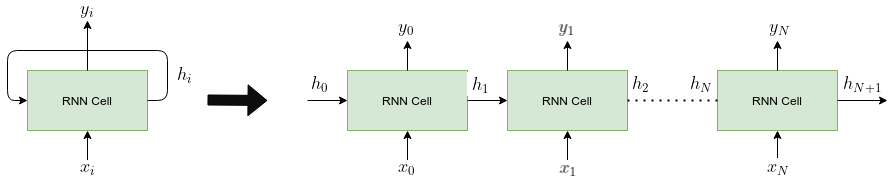
\includegraphics[width=15cm]{./content/materials/rnns.png}
    \caption{Cấu trúc tính toán của RNN}
\end{figure}

Như vậy, mạng RNN có công thức truy hồi được biểu diễn như sau:

\begin{equation}
\begin{split}
    &h_0=0\\
    &h_i=f(W_{hx}*x_i+W_{hh}*h_{i-1}+b_h)\\
    &y_i=g(W_{yh}*hi+b_y)\\
\end{split}
\end{equation}

Với:
\begin{itemize}
    \item \textbf{$h_i$:} Trạng thái ẩn ở bước thứ i
    \item \textbf{$x_i$:} Đầu vào của mạng ở bước thứ i
    \item \textbf{$y_i$:} Đầu ra của mạng ở bước thứ i
    \item \textbf{$W_{hx}$, $W_{hh}$, $W_{yh}$ và $b_h$, $b_y$:} Các trọng số của mạng 
\end{itemize}

Về lý thuyết, mỗi đầu vào của mạng RNN đều cho ra một kết quả ở đầu ra và tạo ra một trạng thái mới cho mạng, sử dụng các kết quả tính toán này như thế nào là tùy vào cách mô hình hóa bài toán và mục tiêu của bài toán. Việc xác định sử dụng kết quả ở đầu ra nào là rất quan trọng vì trọng số của mạng sẽ được cập nhật dựa vào kết quả đó.

Tóm lại, RNN được thiết kế đặc thù cho việc giải quyết dữ liệu dạng chuỗi, với ưu điểm là có khả năng giải quyết chuỗi với độ dài bất định với kích thước mô hình cô định, không phụ thuộc vào đầu vào. Việc tính toán của mạng RNN có xem xét tới thông tin ở quá khứ và chia sẻ trong số trong quá trình tính toán giúp cho mạng giảm số lượng trọng số học và cải thiện tính tổng quát hóa, tránh tình trạng học thuộc. Tuy nhiên, do việc tính toán diễn ra tuần tự nên việc tính toán song song bị hạn chế. Đồng thời RNN cũng có khả năng bị "quên" mất dữ liệu được học trước đó nếu chuỗi dữ liệu quá dài. Để khắc phục vấn đề này, người ta cũng đưa ra cấu trúc LSTM sẽ được trình bà ở phần sau.

\subsubsection{Mạng LSTM}

\subsubsection{Lớp lấy mẫu (Pooling)}

Lớp lấy mẫu thường được sử dụng khi chúng ta muốn giảm bớt kích thước của dữ liệu nhưng vẫn giữ được những đặc trưng nổi bật nhất. Lớp lấy mẫu dùng một cửa sổ thường có kích thước hình vuông $m$x$m$ (thuờng được chọn là 2x2) để quét qua tất cả các ô trên ma trận dữ liệu kích thước $N$x$N$ và thực hiện phép lấy mẫu trên cửa sổ đó. Kết quả cuối cùng sẽ là ma trận có kích thước $\frac{N}{m}$x$\frac{N}{m}$. Tùy vào phép lấy mẫu nào được thực hiện mà kết quả của mỗi lần lấy mẫu sẽ khác nhau. Có hai phép lấy mẫu thường được sử dụng là lấy mẫu lớn nhất (Max Pooling) và lấy mẫu trung bình (Average Pooling). Trong đó, phép lấy mẫu lớn nhất thường được sử dụng để lấy ra đặc trưng nổi bật nhất của dữ liệu, trong khi phép lấy mẫu trung bình thường được dùng để thu nhỏ dữ liệu và trung hòa các đặc trưng xung quanh. Tùy vào mục đích cuối cùng của mạng mà sử dụng phép lấy mẫu sao cho hợp lý.

\begin{figure}[H]
    \centering
    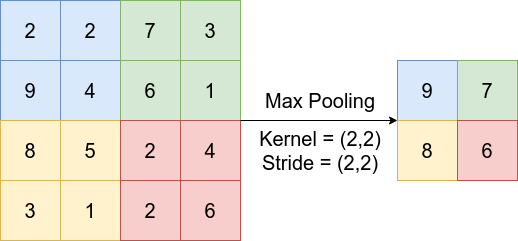
\includegraphics[width=10cm]{./content/materials/max_pooling.png}
    \caption{Ví dụ tính toán lớp lấy mẫu lớn nhất (Max Pooling)}
\end{figure}

\subsubsection{Lớp chuẩn hóa theo bó (Batchnorm)}

Việc huấn luyện mạng học sâu có chiều sâu lớn thường rất khó khăn do càng đi sâu vào mạng, gradient của các trọng số càng giảm và đôi khi tiến rất gần về 0. Do đó, lúc cập nhật trọng số, do gradient xấp xỉ 0 nên trọng số không được cập nhật và điều chỉnh nhiều. Đồng thời, khi huấn luyện mạng, các lớp trong mạng được cập nhật trọng số mà không quan tâm tới sự thay đổi trọng số của các lớp trước nó, và sự thay đổi trọng số này được thực hiện với giả sử là trọng số các lớp trước được giữ nguyên. Nhưng trên thực tế, các trọng số trong tất cả các lớp đều được cập nhật trong quá trình huấn luyện. Vì vậy, lớp chuẩn hóa theo bó được ra đời nhằm mục đích chuẩn hóa đầu ra của các lớp trước nó, vì vậy các lớp phía sau sẽ nhận được đầu vào là các ma trận đã được chuẩn hóa, có giá trị trung bình bằng 0 và độ lệch chuẩn bằng 1 (phân phối Gaussian chuẩn). Việc chuẩn hóa này làm cho việc huấn luyện mạng trở nên ổn định hơn, hạn chế tình trạng triệt tiêu gradient và đẩy quá trình huấn luyện nhanh hơn nhiều lần

\begin{figure}[H]
    \centering
    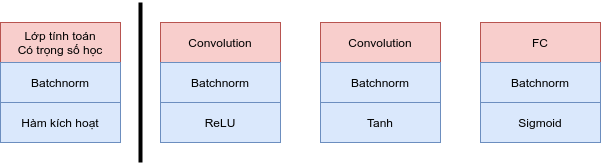
\includegraphics[width=13cm]{./content/materials/batchnorm.png}
    \caption{Một số cách đặt Batchnorm phổ biến}
\end{figure}

Lớp chuẩn hóa theo bó thường được đặt sau một lớp tính toán có trọng số, nhờ đó, khi trọng số của lớp tính toán này được cập nhật và thay đổi, lớp Batchnorm sẽ chuẩn hóa kết quả này, nhờ đó, các lớp sau sẽ nhận được các tín hiệu có phân phối không thay đổi nhiều. Cũng nhờ vậy mà các hàm kích hoạt cũng hoạt động hiệu quả hơn. Do lớp Batchnorm cố gắng chuẩn hóa phân phối xác suất của đầu vào sao cho đầu ra của nó là một phân phối chuẩn có giá trị trung bình bằng 0 và phương sai bằng 1, và các hàm kích hoạt như ReLU, Tanh, Sigmoid đều có điểm cắt tại 0, nên gần như một nữa đầu vào của hàm kích hoạt sẽ nhỏ hơn 0 và nửa còn lại sẽ lớn hơn 0, do đó khi áp dụng các hàm kích hoạt cho phân phối này, các hàm kích hoạt sẽ đạt hiệu quả cao nhất.

\subsubsection{Mạng nơ ron hồi quy tích chập (CRNN)}

Trong xử lý hình ảnh, người ta thường dùng mạng tích chập (CNN), nhưng đối với video là một chuỗi hình ảnh theo thời gian, ta phải xem xét tính chất thay đổi theo thời gian của hình ảnh. Vì vậy, sữ kết hợp của mạng tích chập (CNN) và mạng hồi quy (RNN) tạo ra mạng hồi quy tích chập (CRNN) được dùng để xử lý các dạng dữ liệu theo chuỗi thời gian với phương pháp tích chập.

Mạng nơ ron hồi quy tích chập gồm hai phần chính:
\begin{itemize}
    \item \textbf{Mạng tích chập:} Mạng tích chập sử dụng mạng CNN để rút trích đặc trưng từ dữ liệu được đưa vào mạng. Các lớp được sử dụng trong mạng này bao gồm lớp tích chập, lớp lấy mẫu (Pooling) và lớp chuẩn hóa theo bó (Batchnorm). Theo đó, mạng này rút trích đặc trưng nhờ vào phép tích chập và sắp xếp các đặc trưng này thành chuỗi các đặc trưng có tính chất liên tục theo thời gian.
    \item \textbf{Mạng hồi quy:} Mạng hồi quy thường được sử dụng là LSTM hai hướng (Bidirectional-LSTM) và có thể có nhiều lớp hồi quy. Tại đây, các đặc trưng được rút trích từ mạng tích chập được đưa vào mạng theo tuần tự.
\end{itemize}

\begin{figure}[H]
    \centering
    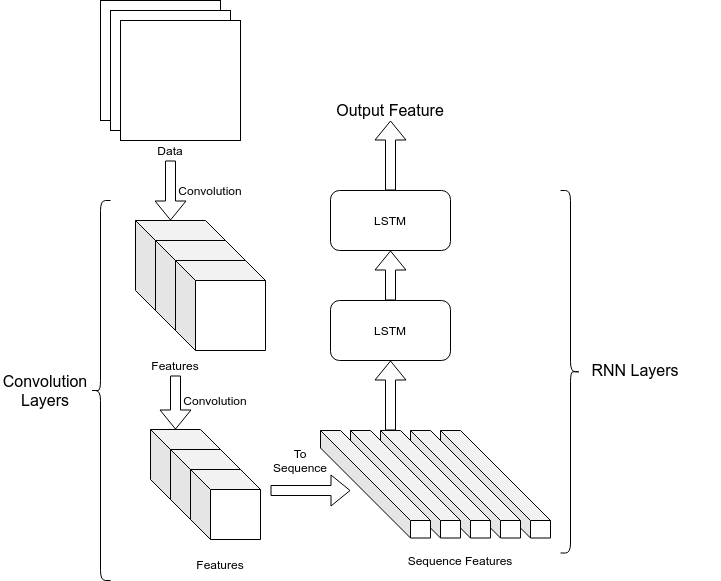
\includegraphics[width=13cm]{./content/materials/crnn.png}
    \caption{Ví dụ về mạng hồi quy tích chập CRNN}
\end{figure}

Ở đầu ra, các đặc trưng sau khi qua mạng hồi quy được sử dụng để đưa ra dự đoán. Cách sử dụng các đặc trưng này tùy thuộc vào yêu cầu của bài toán (tương tự như mạng RNN).

\subsubsection{Mạng nơ ron nối tắt (Residual Network)}

Về mặt kiến trúc, một mạng nơ ron truyền thẳng có khả năng xấp xỉ mọi hàm với dữ liệu huấn luyện được cung cấp, miễn là không vượt quá sức chứa của nó. Tuy nhiên, xấp xủ tốt dữ liệu không phải là mục tiêu duy nhất của một mạng nơ ron, mà như đã nói ở trên, chúng ta cần một mô hình có khả năng tổng quá hóa dữ liệu tốt. Nhờ vào mạng AlexNet, các kiến trúc mạng nơ ron tích chập được chú ý, và từ đó trở đi, các mạng nơ ron được ra đời ngày càng nhiều và chiều sâu của mạng cũng ngày một lớn hơn. Trong khi AlexNet chỉ có 5 lớp tích chập, thì mạng VGG ra đời sau đó có đến 19 lớp, mạng GoogleNet có đến 22 lớp. Như đã nói ở trên, việc tăng độ sâu của mạng có thể làm xảy ra hiện tượng triệt tiêu đạo hàm

\begin{figure}[H]
    \centering
    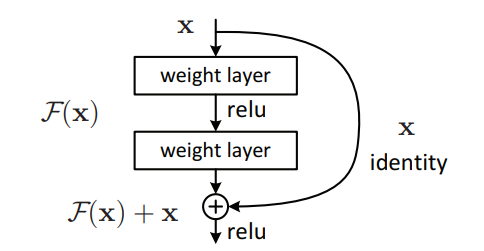
\includegraphics[width=10cm]{./content/materials/residual_orig.png}
    \caption{Cấu trúc của mạng nơ ron nối tắt. Hình ảnh được lấy từ bài báo gốc \cite{residual}}
\end{figure}

Như vậy, nhằm mục đích tạo ra một mạng tích chập có độ sâu lớn nhưng vẫn đảm bảo mạng không bị tình trạng triệt tiêu đạo hàm, cấu trúc mạng nơ ron nối tắt ra đời. Ý tưởng của mạng nối tắt, như cái tên của nó là sử dụng một đường kết nối để nối tắt qua một hay nhiều lớp tích chập, nhằm đem đặc trưng từ các lớp trước để kết họp với các đặc trưng sau khi được rút trích bởi mạng tích chập trong khối nối tắt. Kiến trúc này giúp cho kiến trúc sâu hơn và ít nhất là không kém hơn các kiến trúc nông. Hơn nữa, với kiến trúc này, các lớp sâu phía trong có thêm thông tin từ các lớp ngoài nên sẽ có sự điều chỉnh trọng số hiệu quả hơn.

\begin{figure}[H]
    \centering
    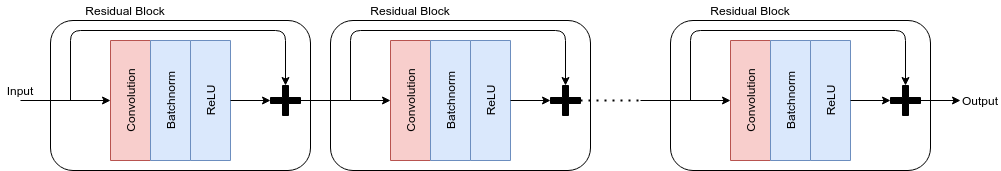
\includegraphics[width=15cm]{./content/materials/residual.png}
    \caption{Mạng nơ ron nối tắt (Residual Network) được dùng trong bài}
\end{figure}

\subsubsection{Các hàm kích hoạt được dùng}

Trong các mạng học sâu, các lớp có chức năng học như lớp tích chập hay lớp kết nối đầy đủ là những biến đổi tuyến tính trên không gian dữ liệu. Do chúng ta cần phải ghép nối nhiều lớp có chức năng học với nhau để có được một mạng có chiều sâu tương đối, đủ lượng trọng số để học được các đặc trưng của dữ liệu. Tuy nhiên như đã nói, các lớp trên là các lớp tuyến tính, nên việc chồng nhiều lớp tuyến tính lên nhau cuối cùng cũng chỉ tạo ra một phép biến đổi tuyến tính trên không gian dữ liệu. Như vậy, nếu chỉ đơn giản là xếp chồng các lớp tuyến tính lên nhau, mô hình học của mạng sẽ chỉ là một phép biến đổi tuyến tính rất đơn giản và không đủ để tổng quát hóa được những bài toán phức tạp. Vì vậy, ta cần một phép biến đổi phi tuyến để phi tuyến hóa mô hình bài toán. 

Các hàm kích hoạt là các phép biến đổi phi tuyến được đưa vào mạng nhằm làm cho mạng trở thành một phép biến đổi phi tuyến và có thể mô hình hóa những bài toán phức tạp hơn. Tuy nhiên, hàm kích hoạt cần phải là một hàm phi tuyến có thể đạo hàm được để đảm bảo mạng được cập nhật trọng số ở bước lan truyền ngược.

\paragraph{Hàm Sigmoid}\mbox{}\\

Hàm Tanh nhận vào một số thực và trả về giá trị trong khoảng (0, 1). Hàm Sigmoid và đạo hàm của nó được biểu diễn bởi hàm số sau:

\begin{equation}
\begin{split}
    & \sigma(x)=\frac{1}{1+e^{-x}}\\
    & \sigma'(x)=\sigma(x)*(1-\sigma(x))\\
\end{split}
\end{equation}

\begin{figure}[H]
    \centering
    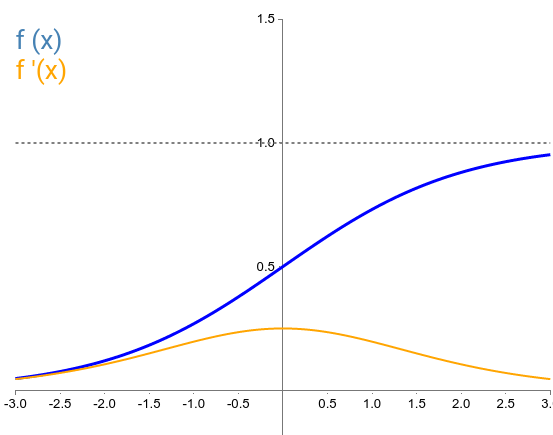
\includegraphics[width=9cm]{./content/materials/sigmoid.png}
    \caption{Hàm Sigmoid}
\end{figure}

Nhìn vào đồ thị của hàm Sigmoid ta thấy, nếu $x$ càng về âm thì $\sigma(x)$ càng tiệm cận về 0 và nếu $x$ càng về dương thì $\sigma(x)$ càng tiến gần đến 1. Tại điểm $x=0$, hàm Sigmoid cho giá trị đạm hàm cực đại và chỉ xấp xỉ bằng 0.3. Với các giá trị đạo hàm khi $x$ càng về âm và càng về dương, đạo hàm của hàm Sigmoid giảm dần về 0. Điểu này gây ra một số bất lợi khi sử dụng Sigmoid để làm hàm kích hoạt:

\begin{itemize}
    \item \textbf{Hàm Sigmoid dễ bị bão hòa:} Như đã nói ở trên, đạo hàm của hàm Sigmoid có giá trị gần 0 khi $x$ quá lớn hoặc quá nhỏ. Trong thực tế, nếu mạng nhận được giá trị khởi động rất lớn hoặc rất nhỏ, mạng này sẽ cho ra giá trị cuối cùng cũng rất lớn hoặc rất nhỏ. Trong lúc lan truyền ngược, đạo hàm của nó sẽ đi qua lớp Sigmoid, như ta đã thấy, nếu $x$ rất lớn hoặc rất nhỏ, đạo hàm của Sigmoid sẽ về gần như bằng 0, và trọng số sẽ được cập nhật rất ít, mạng sẽ rất lâu hội tụ.
    \item \textbf{Hàm Sigmoid dễ bị triệt tiêu đạo hàm:} Ngoài ra, trong trường hợp ngược lại, nếu mạng nhận được trọng số vừa phải, thì lúc này, trong lúc đạo hàm, hàm Sigmoid vẫn cho giá trị đạo hàm rất nhỏ (cao nhất là gần 0.3 tại điểm $x=0$). Nếu sử dụng nhiều lớp Sigmoid trong một mạng học sâu, hiện tượng triệt tiêu đạo hàm sẽ xảy ra.
    \item \textbf{Hàm Sigmoid không đi qua trục tọa độ:} Vì vậy, việc cập nhật các trọng số  của mạng trong lúc lan truyền ngược sẽ luôn đi theo một hướng cùng dương hoặc cùng âm, làm mất đi sự linh hoạt của việc cập nhật trọng số và làm cho mạng khó hội tụ hơn.
\end{itemize}

Trong thực tế, hàm Sigmoid chỉ được sử dụng cho lớp sau cùng của mạng, và được dùng để dự đoán xác suất cho một sự kiện trong bài toán. Nên hạn chế việc sử dụng nhiều lần mạng Sigmoid trên cùng một đường lan truyền vì nó sẽ làm triệt tiêu đạo hàm.

\paragraph{Hàm Tanh}\mbox{}\\

Hàm Tanh nhận vào một số thực và trả về giá trị trong khoảng (-1, 1). Hàm Tanh và đạo hàm của nó được biểu diễn bởi hàm số sau:

\begin{equation}
\begin{split}
    & tanh(x)=\frac{e^x-e^{-x}}{e^x+e^{-x}}=2*\sigma(2x)-1\\
    & tanh'(x)=1-tanh^2(x)\\
\end{split}
\end{equation}

\begin{figure}[H]
    \centering
    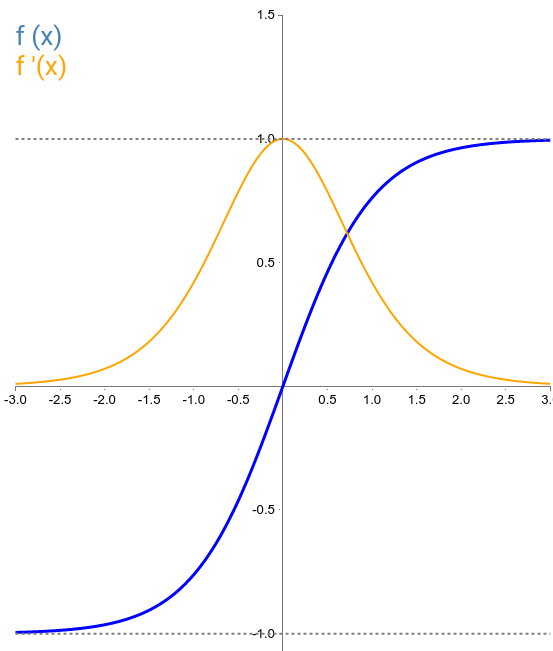
\includegraphics[width=9cm]{./content/materials/tanh.png}
    \caption{Hàm Tanh}
\end{figure}

Nhìn vào đồ thị hàm Thanh ta thấy, hàm Tanh cũng có các tính chất tương tự như hàm Sigmoid: dễ bị bão hòa, dễ bị triệt tiêu đạo hàm. Nhưng nó lại có tính chất đi qua trục tọa độ. Do đó, việc cập nhật trọng số sẽ dễ dàng hơn đối với hàm Tanh. Trên thực tế, giống như hàm Sigmoid, hàm Tanh cũng được dùng để đạt ở những lớp cuối cùng của mạng và cũng không nên đặt nhiều hàm Tanh trên cùng một đường lan truyền để tránh hiện tượng triệt tiêu đạo hàm.

\paragraph{Hàm điểu chỉnh tuyến tính (Rectified Linear Units - ReLU)}\mbox{}\\

Hàm điều chỉnh tuyến tính là hàm kích hoạt đơn giản nhưng mang lại hiệu quả cao. Hàm ReLU và đạo hàm của nó được biểu diễn bởi các hàm số sau:

\begin{equation}
\begin{split}
    & f(x) = max(0,x)\\
    & f'(x) = 
        \begin{cases}
            & 1 \text{ if } x>0\\
            & 0 \text{else}
        \end{cases}
\end{split}
\end{equation}

\begin{figure}[H]
    \centering
    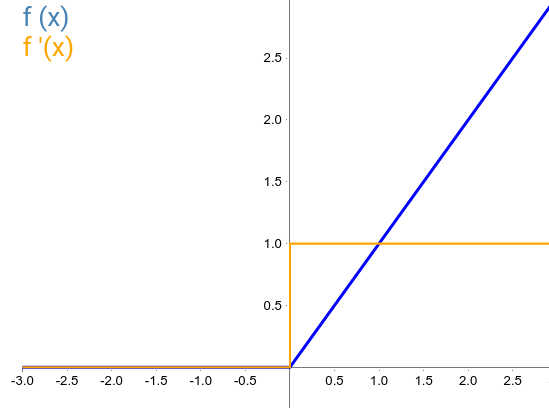
\includegraphics[width=9cm]{./content/materials/relu.png}
    \caption{Hàm ReLU}
\end{figure}

Theo như hàm số trên, ta thấy ReLU chỉ cho phép các giá trị lớn hơn 0 đi qua nó. Như vậy, so với hàm Sigmoid và hàm Tanh, ReLU sẽ không xuất hiện vấn đề triệt tiêu đạo hàm. Đồng thời, việc tính toán cho hàm ReLU cũng diễn ra nhanh hơn đáng kể. Tuy nhiên, ReLU cũng có một nhược điểm là nếu $x$ có giá trị nhỏ hơn 0, nó sẽ được hàm ReLU cho kết quả bằng 0. Vì vậy, giá trị tính toán tại $x$ sẽ không có ý nghĩa cho các lớp tiếp theo, và các hệ số học tương ứng từ đó cũng không được cập nhật trong quá trình lan truyền ngược. Hiện tượng này gọi là \textit{Dying ReLU}.

\subsection{\texorpdfstring{Cấu trúc mạng tạo sinh đối nghịch (Generative Adversarial Networks - GANs}{gans})}

\subsubsection{Mạng GANs}\label{sec:base_knowledge_gans}
Vào năm 2014, Ian Goodfellow và cộng sự đã xuất bản một bài báo \cite{gans_base} giới thiệu về mạng tạo sinh đối nghịch (GANs). Mạng GANs đã cho phép máy tính có thể tạo sinh ra dữ liệu chân thật, không phải chỉ bằng một mạng nơ ron, mà là hai mạng nơ ron độc lập. Tuy mạng GANs không phải là mạng nơ ron đầu tiên có chức năng tạo sinh dữ liệu, nhưng kết quả tạo sinh nó mang lại thì có chất lượng vượt xa tất cả các công bố trước đây. Nó đã đạt được những kết quả mà trước đây, người ta không nghĩ là mạng nơ ron học sâu có thể làm được. Mạng GANs có thể tạo sinh hình ảnh giả với độ chân thật cao, và có thể so sánh với máy chụp ảnh, biến những hình vẽ thành ảnh chụp nghệ thuật, hay biến những thước phim có hình ảnh của những con ngựa thành những thước phim có hình ảnh của những con ngựa vằn. Và nó làm những điều này mà không cần đến những dữ liệu được đánh nhãn.

\begin{figure}[H]
    \centering
    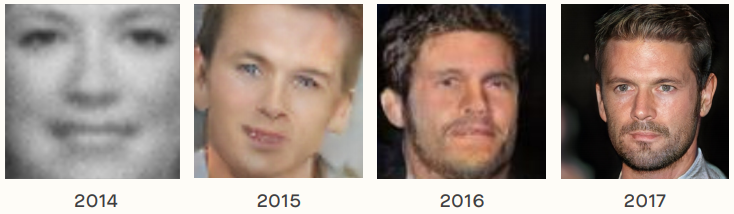
\includegraphics[width=15cm]{./content/materials/gans-faces.png}
    \caption{Việc tạo sinh mặt người dùng mạng GANs qua các năm \cite{gans_faces}}
\end{figure}

Mạng tạo sinh đối nghịch (GANs) là một loại mạng thần kinh học sâu dùng để tạo sinh dữ liệu mà nó được học. Mạng tạo sinh đối nghịch bao gồm hai mạng nhỏ hơn là mạng tạo sinh (Generator) và mạng phân biệt (Discriminator). Mạng tạo sinh được huấn luyện để sinh ra dữ liệu mới, trong khi mạng phân biệt được huấn luyện để phân biệt dữ liệu nào là dữ liệu thật được lấy từ tập dữ liệu huấn luyện, dữ liệu nào là dữ liệu giả được sinh ra bởi mạng tạo sinh. Ví dụ, chúng ta muốn tạo sinh các bức họa có phong cách vẽ giống với Leonardo da Vinci, ta có thể dùng tập dữ liệu các bộ tranh vẽ của Leonardo da Vinci để huấn luyện cho mạng. Mạng tạo sinh sẽ cố gắng học cách tạo sinh ra các bức họa giống với phong cách của Leonardo da Vinci nhất, trong khi mạng phân biệt cố  học cách phân biệt các bức họa thật giả, với ảnh thật là các ảnh lấy trực tiếp từ dữ liệu huấn luyện, còn ảnh giả là các bức ảnh được tạo ra bởi mạng tạo sinh.

\subsubsection{Cách hoạt động của mạng GANs}
\begin{figure}[H]
    \centering
    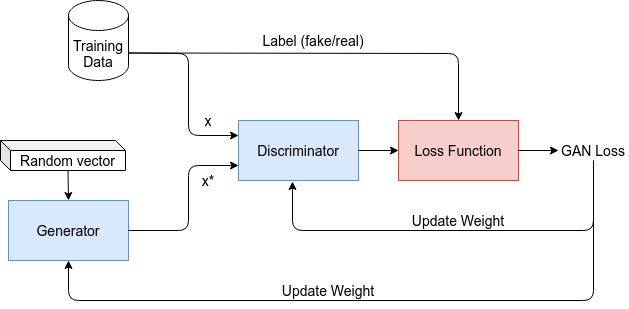
\includegraphics[width=15cm]{./content/materials/gans-pure.png}
    \caption{Cấu trúc mạng GANs thông thường}
    \label{fig:pure-gans}
\end{figure}

Như vậy, mục đích của mạng tạo sinh là tạo ra những dữ liệu có cùng tính chất với dữ liệu được đưa vào để huấn luyện cho nó, những dữ liệu được sinh ra phải chân thật đến nỗi không thể phân biệt được với dữ liệu thật. Mạng tạo sinh có thể được xem như một phiên bản ngược của mạng nhận diện (Object Recognition Networks), trong khi mạng nhận diện có chức năng học những chi tiết, đặc trưng trên những tấm ảnh nó được học qua để tìm ra được vật thể trên ảnh. Thì với mạng tạo sinh, thay vì học các chi tiết, đặc trưng của vật thể, nó học cách để tạo ra các chi tiết, đặc trưng đó với đầu vào chỉ đơn giản là một vec tơ được tạo sinh ngẫu nhiên bằng phân phối chuẩn (đói với mạng GANs truyền thống). 

Việc học cách tạo sinh dữ liệu được mạng tạo sinh thực hiện nhờ vào phản hồi của mạng phân biệt Discriminator. Mục đích của mạng phân biệt là tìm cách phân biệt dữ liệu đầu vào cũa nó, dữ liệu nào được tạo sinh và dữ liệu nào là dữ liệu thật. Do vậy, mỗi lần mạng phân biệt bị đánh lừa bởi mạng tạo sinh (nhận nhầm dữ liệu tạo sinh là dữ liệu thật), mạng tạo sinh biết là nó đang làm đúng. Và ngược lại, mỗi lần mạng phân biệt bắt được đúng dữ liệu giả, thông tin này sẽ được đưa về cho mạng tạo sinh và nó sẽ phải cập nhật lại trọng số để tạo sinh dữ liệu chân thật hơn.

Mạng phân biệt cũng dần được cải thiện qua mỗi lần nó phân biệt sai dữ liệu. Với hàm mất mát Binary Cross Entropy, nó tính toán được khoảng cách từ dự đoán của chính nó đến kết quả thực và từ đó thay đổi trọng số của mạng để dự đoán của nó ngày càng phù hợp hơn với phân phối dữ liệu. Cứ như vậy, mạng tạo sinh càng ngày càng sinh ra dữ liệu chân thực hơn nhằm mục đích đánh lừa mạng phân biệt, nhưng mạng phân biệt cũng ngày càng trở nên tốt hơn trong việc phân biệt dữ liệu thật - giả.

\subsubsection{Huấn luyện mạng GANs}

Do mạng GANs là tổng hợp của hai mạng tạo sinh và mạng phân biệt, nên cách huấn luyện mạng cũng có sự khác biệt so với các loại mạng khác. Khi huấn luyện mạng GANs, ta sẽ đi huấn luyện cho cả hai mạng tạo sinh và phân biệt cùng một lúc. Chi tiết các bước huấn luyện một mạng GANs truyền thống được miêu tả ở Hình \ref{fig:pure-gans} như sau:

Với mỗi lượt huấn luyện, ta lần lượt thực hiện:
\begin{itemize}
    \item Huấn luyện mạng phân biệt:
    \begin{itemize}
        \item Lấy một vài mẫu dữ liệu thật ($x$) từ tập dữ liệu huấn luyện
        \item Lấy mẫu ngẫu nhiên dựa trên phân phối chuẩn để tạo ra véc tơ $z$, đưa véc tơ $z$ vào mạng tạo sinh để tạo ra dữ liệu giả ($x^*$)
        \item Sử dụng mạng phân biệt để phân biệt $x$ và $x^*$
        \item Tính toán hàm mất mát của mạng phân biệt và thực hiện lan truyền ngược trên mạng phân biệt nhằm tối thiểu hóa hàm mất mát
    \end{itemize}

    \item Huấn luyện mạng tạo sinh:
    \begin{itemize}
        \item Lấy mẫu ngẫu nhiên dựa trên phân phối chuẩn để tạo ra véc tơ $z$, đưa véc tơ $z$ vào mạng tạo sinh để tạo ra dữ liệu giả ($x^*$)
        \item Sử dụng mạng phân biệt để phân biệt dữ liệu giả vừa được tạo sinh
        \item Tính toán hàm mất mát của mạng phân biệt và thực hiện lan truyền ngược trên mạng tạo sinh nhằm tối đa hóa hàm mất mát
    \end{itemize}
\end{itemize}

\subsubsection{Điểm cân bằng trong huấn luyện mạng GANs}

Vậy khi nào thì việc huấn luyện mạng GANs nên được dừng lại? Làm sao và dựa vào dấu hiệu nào để biết được mạng GANs đã hội tụ? Với các mạng nơ ron thông thường khác, ta thường có các thông số rõ ràng và những mục tiêu rõ ràng để biết khi nào thì dừng việc huấn luyện. Ví dụ như với mạng phân lớp, ta có thể chia dữ liệu huấn luyện thành tập để học và tập để kiểm thử. Khi giá trị hàm mất mát trên tập kiểm thử bắt đầu tệ đi là lúc ta nên dừng quá trình huấn luyện mạng vì mạng đã bắt đầu học thuộc dữ liệu. Trong mạng GANs, hai mạng tạo sinh và phân biệt có hai mục tiêu trái ngược nhau. Bên tạo sinh cố gắng tạo ra dữ liệu thật chân thật để đánh lừa bên phân biệt, trong khi bên phân biệt ngày càng cải thiện bản thân để phân biệt thật - giả tốt hơn. Như vậy, nếu bên tạo sinh có giá trị hàm mất mát thấp hơn, thì giá trị hàm mất mát của bên phân biệt sẽ cao lên và ngược lại.

Như vậy, ta có thể thấy đây là một trò chơi có tổng bằng 0 (zero-sum game), ở đó, bên này được bao nhiêu thì bên kia mất bấy nhiêu. Tất cả mọi zero-sum game đều có một điểm cân bằng Nash (Nash equilibrium) mà tại đó, cả hai bên đều không thể làm gì để cải thiện tình hình chung. Mạng GANs đạt được trạng thái cân bằng Nash khi những điều kiện sau đây được thỏa mãn:
\begin{itemize}
    \item Mạng tạo sinh có thể tạo ra dữ liệu giả không thể phân biệt được với dữ liệu thật
    \item Mạng phân biệt có thể dự đoán một cách ngẫu nhiên một mẫu dữ liệu là thật hay giả (độ chính xác của bộ phân biệt đạt 50\%)
\end{itemize}
Khi trạng thái này xảy ra, mạng phân biệt không còn khả năng để dự đoán mẫu dữ liệu nào là thật, mẫu dữ liệu nào là giả, vì vậy nó không thể giúp ích gì thêm cho mạng tạo sinh nữa. Mạng tạo sinh cũng không còn khả năng cải thiện hơn, vì dữ liệu nó sinh ra đã không còn có thể được nhận diện bởi mạng phân biệt. Vì vậy, khi ở trạng thái này, mạng GANs đã hội tụ và ta có thể ngừng việc huấn luyện tại đây.

Nhưng trên thực tế, trạng thái cân bằng Nash dường như không thể đạt được bởi sự phức tạp và rộng lớn của không gian dữ liệu, với số chiều rất lớn và là tập hơn của các hàm tuyến tính, hàm kích hoạt, lấy mẫu, và đôi khi là hàm xác suất,... tất cả những hàm đó tạo nên một không gian không lồi, và với việc sử dụng các giải thuật tối ưu như SGD và Adam, đôi khi ta chỉ tìm được các điểm tối ưu cục bộ. Trên thực tế, sự hội tụ của mạng GANs vẫn còn là một câu hỏi mở cho ngành trí tuệ nhân tạo.

\subsection{\texorpdfstring{Đặc trưng MFCC (mel-frequency cepstrum coefficients) của dữ liệu âm thanh}{mfcc}}

Đầu tiên, ta sẽ đi qua định nghĩa về cepstrum. Cepstrum là một đặc trưng quan trọng để phân biệt các nguyên âm trong xử lý tiếng nói. Về mặt ý nghĩa, cepstrum giúp phân biệt các nguyên âm do nó là đặc trưng được sinh ra từ tần số của âm thanh. Khi con người cất tiếng nói, một nguyên âm nào đó khi phát ra sẽ được cuốn họng rung để tạo ra tần số cơ bản, khoang mũi, miệng, lưỡi và môi giống như các bộ lọc âm thanh để tạo ra các tần số mới, và các đỉnh cực đại của các tần số khác nhau trong tín hiệu tiếng nói quyết định âm được nói ra là âm gì. Để chuyển sự biểu diễn âm thanh từ miền thời gian sang miền tần số, người ta thường dùng biến đổi Fourier. Một âm thanh tiếng nói khi được biến đổi Fourier sẽ tạo ra một hàm số thể hiện biên độ của các tần số khác nhau. Đồ thị này sẽ có các điểm cực đại, và các điểm cực đại này là đặc trưng cho nguyên âm vừa được nói ra (như đã nói ở trên). Khi hàm biến đổi Fourier này được đưa về dạng hàm trơn, ta gọi đó là cepstrum. Các nguyên âm khác nhau thì mỗi nguyên âm sẽ có một dạng biểu diễn đồ thị cepstrum khác nhau, phân biệt khá rõ ràng về số đỉnh và khoảng cách giữa các đỉnh.

Tai nghe của con người có một đặc điểm quan trọng, chúng hoạt động như những bộ lọc âm thanh, nhạy cảm hơn với các âm ở tần số thấp và ít nhạy hơn với âm thanh ở tần số cao. Vì vậy, bộ lọc Mel ra đời nhằm xử lý các âm thanh tiếng nói để trích xuất các đặc trưng sao cho phù hợp với cách nghe của con người. Theo đó, các giá trị tần số nhỏ hơn 1kHz sẽ được lọc với bộ lọc tuyến tính, điều này phù hợp với lý thuyết là tai người nhạy cảm với âm thanh có tần số thấp. Dải tần số trên 1kHz được lọc với bộ lọc phi tuyến và bộ lọc thưa dần khi lên đến các tần số cao hơn.

MFCC là một đặc trưng âm thanh và được tạo ra nhằm mục đích duy nhất là dùng cho giọng nói con người. Vì vậy, MFCC thường được sử dụng trong các bài toán nhận dạng giọng nói hay phân loại giọng nói. MFCC sẽ cho ra kết quả là các hệ số của cepstrum được lấy từ bộ lọc Mel sau khi xử lý phổ của âm thanh giọng nói.

\section{\texorpdfstring{Phương pháp nghiên cứu}{methodology}}
% Trình bày chi tiết về ý tưởng, các mô hình toán, các chứng minh nếu có. Đồng thời trình bày các bước thực hiện và khảo sát, kiểm nghiệm kết quả nghiên cứu. Mô tả kết quả nghiên cứu khi thử nghiệm với nhiều tập dữ liệu và những độ khó khác nhau.

\subsection{Ý tưởng thực hiện luận văn}

Nhắc lại yêu cầu bài toán: Tạo sinh video khuôn mặt người đang nói dựa trên một hình ảnh tĩnh chứa mặt người mẫu và một đoạn âm thanh chứa tiếng nói. Qua yêu cầu bài toán ta thấy, đầu vào của hệ thống có tính chất khác với đầu ra, sử dụng hình ảnh tĩnh và âm thanh để tạo ra hình ảnh chuyển động. Một số yêu cầu quan trọng khác quyết định chất lượng của chuỗi hình ảnh được tạo sinh ra cũng cần được chú ý. Đó là:
\begin{itemize}
    \item Hình ảnh phải chân thật, rõ ràng, thể hiện được đúng hình dáng gương mặt người đang nói, không bị méo mó, dị dạng.
    \item Chuỗi hình ảnh được tạo sinh cần phải giữ được đặc trưng gương mặt trong ảnh mẫu. Có nghĩa là, người xem vẫn có thể nhận ra được mặt người đang nói trong video được tạo sinh chính là người trong hình ảnh ban đầu
    \item Khẩu hình miệng khi chuyển động phải khớp với âm thanh được nói ra. Sự chuyển động của môi và miệng trong video được tạo sinh phải thể hiện được cách phát âm từ được nói gần như trong thực tế
\end{itemize}

Dựa theo yêu cầu bài toán, ta cần tìm kiếm một phương pháp để kết hợp đặc trưng âm thanh và hình ảnh lại với nhau, sau đó chuyển đổi đặc trưng này thành video. Để mang lại sự trung thực, sắc nét cho hình ảnh được tạo sinh cũng như lưu giữ được các đặc trưng khuôn mặt người trong hình ảnh ban đầu, chiến thuật của ta là sẽ dựa hoàn toàn trên hình ảnh ban đầu để tạo sinh các khung hình khác trong video. Như vậy, với mỗi khung hình ở mỗi thời điểm $t$ trên video, ta cần phải tìm kiếm sự thay đổi của khung ảnh tại thời điểm đó so với hình ảnh tĩnh được cho ban đầu. Sau đó, ta thực hiện biến đổi hình ảnh được cho ban đầu thành hình ảnh ở khung hình tại thời điểm $t$. Như vậy, câu hỏi đặt ra là ta cần phải thay đổi tại vùng nào trên ảnh mẫu và tại những vùng đó ta sẽ thay đổi như thế nào, thay đổi nhiều hay ít.

Sự thay đổi của hình ảnh được quyết định phần nhiều bởi chuỗi âm thanh được đưa vào hệ thống. Âm thanh giọng nói quyết định khẩu hình miệng và các biểu cảm trên gương mặt. Đôi khi, giọng nói còn có thể quyết định cách chuyển động của đầu. Tuy nhiên, tuy giọng nói góp phần lớn khi định hình sự thay đổi trên gương mặt trong lúc nói, ảnh mẫu ban đầu cũng quyết định phần nào các thay đổi đó. Hình ảnh ban đầu cung cấp thông tin về nhận dạng khuôn mặt, về những đặc điểm của các bộ phận trên gương mặt người nói, về vị trí của mắt, mũi, miệng để định hình cách âm thanh thay đổi hình dạng gương mặt trong lúc nói.

\begin{figure}[H]
    \centering
    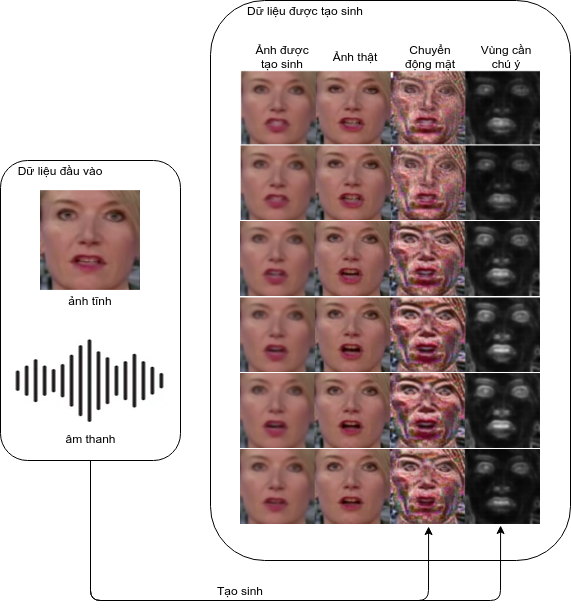
\includegraphics[width=12cm]{./content/materials/idea.png}
    \caption{Ý tưởng về tạo sinh chuỗi hình ảnh chuyển động cho mặt người đang nói}
\end{figure}

Ý tưởng giải quyết bài toán được thể hiện ở hình trên. Chúng ta sẽ tạo ra một hệ thống có khả năng trích xuất đặc trưng của hình ảnh tĩnh ban đầu và âm thanh giọng nói để tạo ra hình ảnh chuyển động của mặt. Tuy nhiên, hình ảnh chuyển động mặt này không hoàn toàn được sử dụng, mà song song với nó, ta tạo ra một mặt nạ tương ứng. Mặt nạ này chỉ chú ý tới một số khu vực trên hình ảnh chuyển động mặt được tạo sinh. Những vùng màu đen là những vùng không được chú ý đến trên ảnh chuyển động vừa được sinh ra, ngược lại, các vùng có màu trắng càng sáng thì càng được chú ý. Như vậy, mặt nạ chú ý sẽ cho ta biết ta nên thay đổi những vùng nào trên gương mặt tại thời điểm $t$ tương ứng với tiếng nói ở thời điểm đó. Đồng thời, hình ảnh chuyển động mặt được tạo sinh song song cho ta biết ta phải thay đổi như thế nào ở những điểm được chú ý. Ở những điểm không được chú ý còn lại, ta sẽ thay thế bằng các điểm ảnh trong ảnh gốc ban đầu. Nhờ vậy, ta có thể bảo toàn được nhận dạng của người nói trong quá trình tạo sinh bằng việc chỉ tìm ra những điểm thay đổi trên gương mặt thay vì cố gắng tìm cách tạo sinh toàn bộ gương mặt của người nói.

\subsection{Mô hình hóa bài toán}

Như phân tích ở phần trên, âm thanh sẽ đóng góp phần lớn vào việc tạo sinh chuyển động cho khuôn mặt. Tuy nhiên, ta thấy dữ liệu dạng sóng biên độ - thời gian của âm thanh dường như không có mối liên hệ tốt với chuyển động trên gương mặt. Vì thế, một bước trích xuất đặc trưng âm thanh để tạo ra một đặc trưng gần gũi hơn với những chuyển động tương ứng trên gương mặt là một bước cần thiết để việc tạo sinh hình ảnh có thể tạo ra những hình ảnh chất lượng tốt và có được những chuyển động chính xác. Do đó, ta sẽ chuyển âm thanh thành một dạng thể hiện khác, đó là các cột mốc trên gương mặt (Facial Landmark). Cột mốc trên mặt gồm 68 điểm trên không gian hai chiều. Mỗi điểm đánh dấu một vị trí trên gương mặt.

\begin{figure}[H]
    \centering
    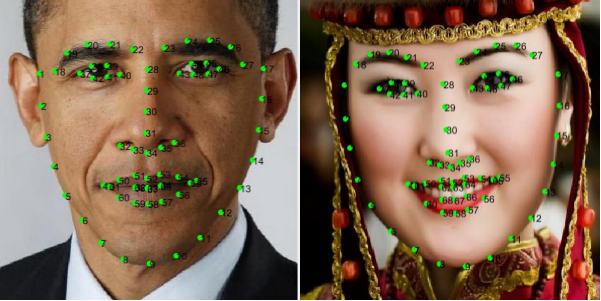
\includegraphics[width=10cm]{./content/materials/landmark_intro.png}
    \caption{Các điểm cột mốc trên khuôn mặt. Hình ảnh được lấy từ bài báo \cite{landmark}}
\end{figure}

Như vậy, từ đoạn âm thanh có chứa tiếng nói và hình ảnh ban đầu, ta sẽ tạo sinh ra một chuỗi cột mốc khuôn mặt để thay thế cho âm thanh làm căn cứ cho những chuyển động trên gương mặt cho phần mạng phía sau. Cấu trúc tổng quát của hệ thống được thế hiện ở Hình \ref{fig:common_architecture}.

\begin{figure}[H]
    \centering
    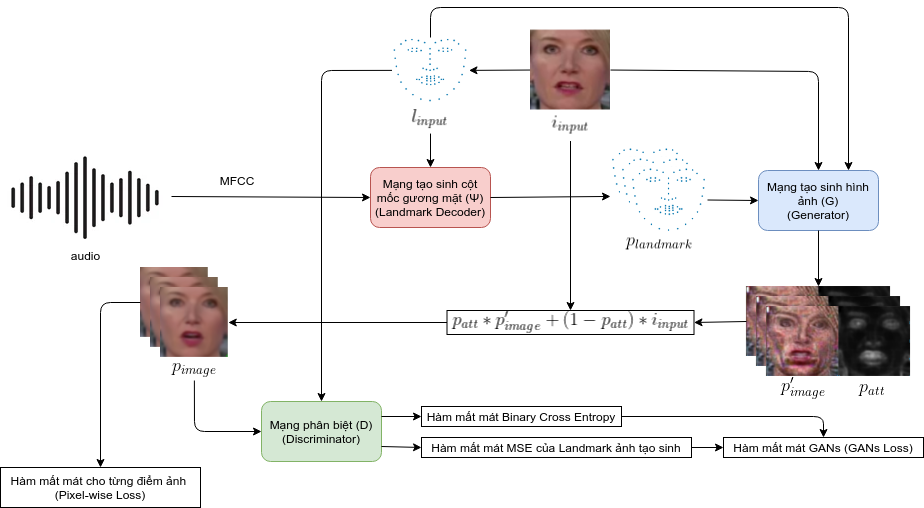
\includegraphics[width=15cm]{./content/materials/common_architecture.png}
    \caption{Cấu trúc tổng quát của hệ thống}
    \label{fig:common_architecture}
\end{figure}

Theo như kiến trúc được thể hiện ở Hình \ref{fig:common_architecture}, hệ thống sẽ trích xuất đặc trưng cột mốc $l_{input}$ trên gương mặt trong hình mẫu $i_{input}$. Sau đó, đặc trưng MFCC sẽ được trích xuất từ âm thanh đầu vào. Đặc trưng MFCC và $l_{input}$ sẽ được đưa vào mạng tạo sinh cột mốc gương mặt (Landmark Decoder). Mạng này kết hợp hai đặc trưng trên với nhau để dự đoán chuỗi các cột mốc gương mặt người khi nói đoạn âm thanh được đưa vào hệ thống ($p_{landmark}$). Từ thời điểm này, âm thanh không còn được sử dụng để tạo sinh hình ảnh mặt người, chuỗi những điểm cột mốc gương mặt $p_{landmark}$ sẽ thay thế cho đặc trưng âm thanh trong những bước xử lý tiếp theo. Như vậy, ta đã tách rời được dữ liệu âm thanh so với phần tạo sinh hình ảnh, và cung cấp cho phần mạng phía sau thông tin dễ học hơn, giàu thông tin hữu ích hơn và ít nhiễu hơn. 

Phần tiếp theo trong hệ thống là cặp mạng tạo sinh (Generator) và phân biệt (Discriminator) tạo nên mạng GANs như đã trình bày ở phần \ref{sec:base_knowledge_gans}. Tuy nhiên, đây không phải là mạng GANs truyền thống mà là mạng GANs có điều kiện (Conditional GANs). Thay vì tạo sinh dữ liệu bằng một véc tơ được sinh ra ngẫu nhiên theo phân phối chuẩn, mạng GANs có điều kiện dựa vào một điều kiện đầu để tạo sinh dữ liệu. Trong luận văn này, mạng GANs có điều kiện tạo sinh dữ liệu với điều kiện đầu vào là $i_{input}$, $l_{input}$ và $p_{landmark}$.

Bài toán mà mạng tạo sinh phải giải là đối với mỗi khung ảnh được tạo sinh để phù hợp với giọng nói được cho, ta phải thay đổi hình ảnh gốc $i_{input}$ ở những vị trí nào, và tại vị trí đó, ta phải thay đỏi nó như thế nào để sinh ra được hình ảnh mới? Mạng tạo sinh hình ảnh với đầu vào là hình ảnh mẫu $i_{input}$, cột mốc của gương mặt của hình ảnh mẫu $l_{input}$ và chuỗi cột mốc gương mặt vừa được tạo sinh $p_{landmark}$ có chức năng tạo sinh ra hai chuỗi dữ liệu $p_{att}$ và $p'_{image}$ tương ứng để trả lời cho câu hỏi trên. Chuỗi hình ảnh $p_{att}$ và $p'_{image}$ có cùng chiểu dài và kích thước hình ảnh. Chuỗi hình ảnh $p_{att}$ thể hiện những điểm cần thay đổi trên ảnh gốc và mức độ thay đổi tại điểm đó. Chuỗi dữ liệu còn lại là chuỗi $p'_{image}$ thể hiện những thay đổi trên ảnh gốc để phù hợp với tiếng nói trong âm thanh. Chuỗi $p'_{image}$ có cấu trúc hình ảnh là gương mặt người, có sự thay đổi theo trục thời gian tương ứng với những chuyển động trên gương mặt để phù hợp với giọng nói. Tuy nhiên đây không phải là hình ảnh hoàn chỉnh của gương mặt, chỉ một vài chi tiết cần thiết trên chuỗi $p'_{image}$ được lấy ra và ghép vào ảnh gốc $i_{input}$ để tạo ra hình ảnh cuối cùng. Cũng vì vậy, $p'_{image}$ là chuỗi hình ảnh được sinh ra để cho ta biết hình ảnh gốc nên thay đổi như thế nào. 

Cuối cùng, ta cần phải kết hợp hình ảnh ban đầu $i_{image}$ và chuỗi hình ảnh vừa được sinh ra là $p'_{image}$ và $p_{att}$ lại để tạo thành chuỗi hình ảnh hoàn chỉnh $p_{image}$. Có thể gọi $p_{att}$ là một mặt nạ chú ý (attention map), mặt nạ này có giá trị các điểm ảnh trong khoảng từ 0 đến 1. Với điểm ảnh càng gần về 0, điểm ảnh cùng vị trí trong $i_{input}$ càng được sử dụng nhiều, điểm ảnh cùng vị trí trong $p'_{image}$ càng ít được sử dụng. Và ngược lại, nếu điểm ảnh trong $p_{att}$ càng gần về 1, điểm ảnh cùng vị trí trong $i_{input}$ càng ít được sử dụng, điểm ảnh cùng vị trí trong $p'_{image}$ càng được sử dụng nhiều. Công thức tạo thành $p_{image}$ được biểu diễn như sau:

\begin{equation}
    p_{image}=p_{att}*p'_{image}+(1-p_{att})*i_{input}
\end{equation}

Hình ảnh hoàn chỉnh được tạo sinh $p_{image}$ sau đó được đem đi so sánh với chuỗi hình ảnh trong video gốc để tính giá trị mất mát L1 cho chuỗi hình ảnh tạo sinh. Giá trị mất mát này được lan truyền ngược để cập nhật các trọng số trong mạng tạo sinh. Chuỗi hình ảnh hoàn chỉnh cũng được đưa vào bộ phân biệt (Discriminator) để bộ phân biệt dự đoán xem chuỗi hình ảnh này là ảnh được tạo sinh (chuỗi hình ảnh giả) hay chuỗi hình ảnh này là hình ảnh được lấy từ tập dữ liệu thật, sai sót của bộ phân biệt được biểu diễn bằng hàm Binary Cross Entropy. Đồng thời bộ phân biệt cũng dựa vào chuỗi hình ảnh được đưa vào và cột mốc gương mặt của ảnh mẫu $l_{input}$ để cố gắng sinh ra một chuỗi cột mốc gương mặt tương ứng với chuỗi hình ảnh $p_{image}$ được đưa vào mạng. Chuỗi cột mốc gương mặt vừa được sinh ra này sẽ được so sánh với chuỗi cột mốc gương mặt được rút trích trực tiếp từ chuỗi hình ảnh trong video gốc. Sự sai khác trong hai chuỗi cột mốc gương mặt được tính bằng hàm mất mát MSE. Điều này có nghĩa, chuỗi hình ảnh được tạo sinh $p_{image}$ phải rút trích được một chuỗi cột mốc gương mặt sao cho giống nhất với chuỗi cột mốc gương mặt trong video gốc. Tổng hợp của giá trị mất mát MSE và Binary Cross Entropy vừa nêu, ta được hàm mất mát GANs chung của mạng GANs. Giá trị mất mát GANs này được lan truyền ngược để cập nhật trọng số cho cả mạng tạo sinh và mạng phân biệt.

\subsection{Các tập dữ liệu được sử dụng}
\subsubsection{Tập dữ liệu GRID \cite{grid}}

Tập dữ liệu GRID là tập dữ liệu 

\begin{figure}[H]
    \centering
    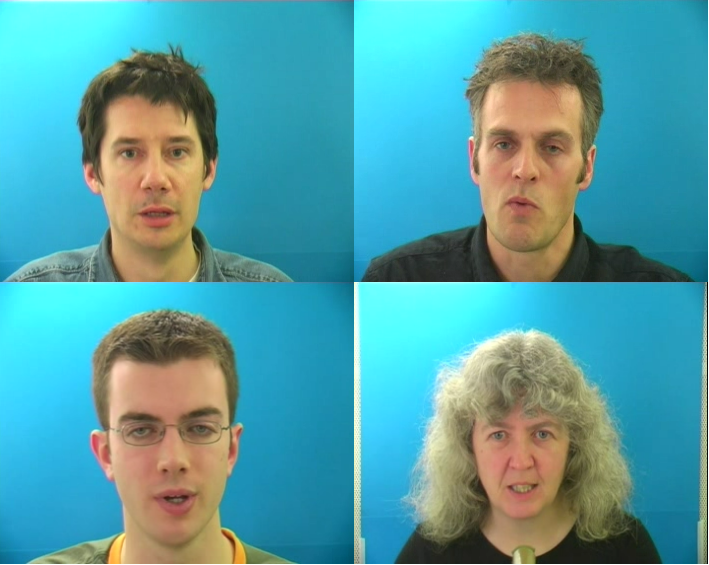
\includegraphics[width=12cm]{./content/materials/grid.png}
    \caption{Ảnh trích xuất từ các video trong tập dữ liệu GRID}
\end{figure}

\subsubsection{Tập dữ liệu LRW \cite{lrw}}

\begin{figure}[H]
    \centering
    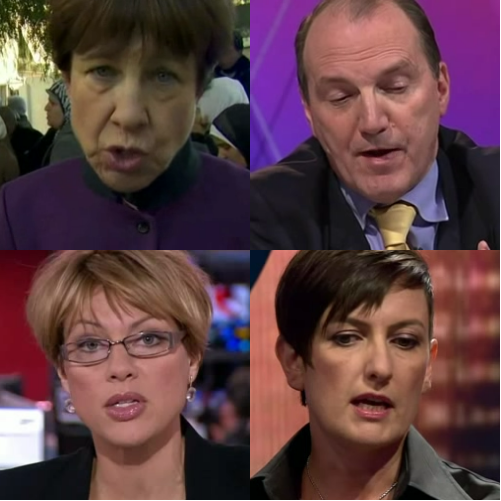
\includegraphics[width=12cm]{./content/materials/lrw.png}
    \caption{Ảnh trích xuất từ các video trong tập dữ liệu LRW}
\end{figure}

\subsection{Tiền xử lý dữ liệu}

Ta có thể thấy, phần âm thanh ta chú ý đến chỉ là tiếng nói của con người và muốn loại bỏ các tạp âm. Tần số âm thanh của giọng nói con người dao động trong khoảng từ 20Hz đến 20kHz, và theo như phương pháp lấy mẫu Nyquist, để lấy mẫu một tín hiệu có tần số $x$(Hz), thì bộ lấy mẫu phải lấy mẫu ở tần số $2x$(Hz). Như vậy, khi thu âm, để thu được âm thanh mà con người có thể nghe được, người ta phải lấy mẫu ở tần số 40kHz. Trên thực tế, trong việc ghi âm, người ta thường lấy mẫu ở tần số 44.1kHz, và đây đã trở thành tiêu chuẩn chung, và hầu hết các video có âm thanh thì âm thanh trong video phần lớn được lấy mẫu ở tần số này.

\subsection{Cấu trúc tổng quát của hệ thống}

\subsection{Cấu trúc của bộ giải mã landmark của khuôn mặt (Landmark Decoder)}

\begin{figure}[H]
    \centering
    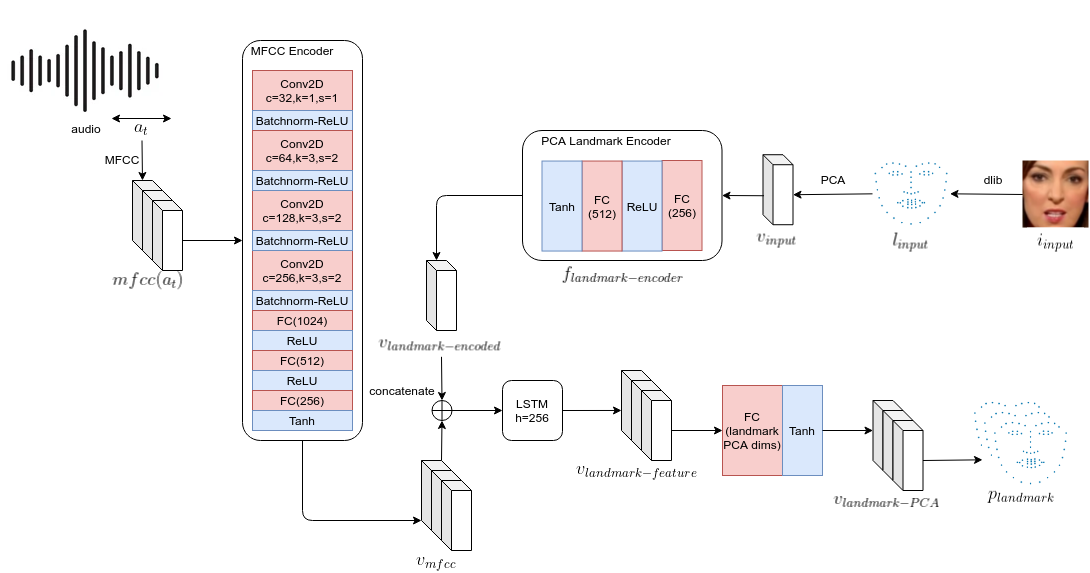
\includegraphics[width=15cm]{./content/materials/landmark_decoder.png}
    \caption{Cấu trúc của bộ giải mã landmark của khuôn mặt (Landmark Decoder)}
\end{figure}



\subsection{Cấu trúc của bộ tạo sinh hình ảnh (Generator)}

\begin{figure}[H]
    \centering
    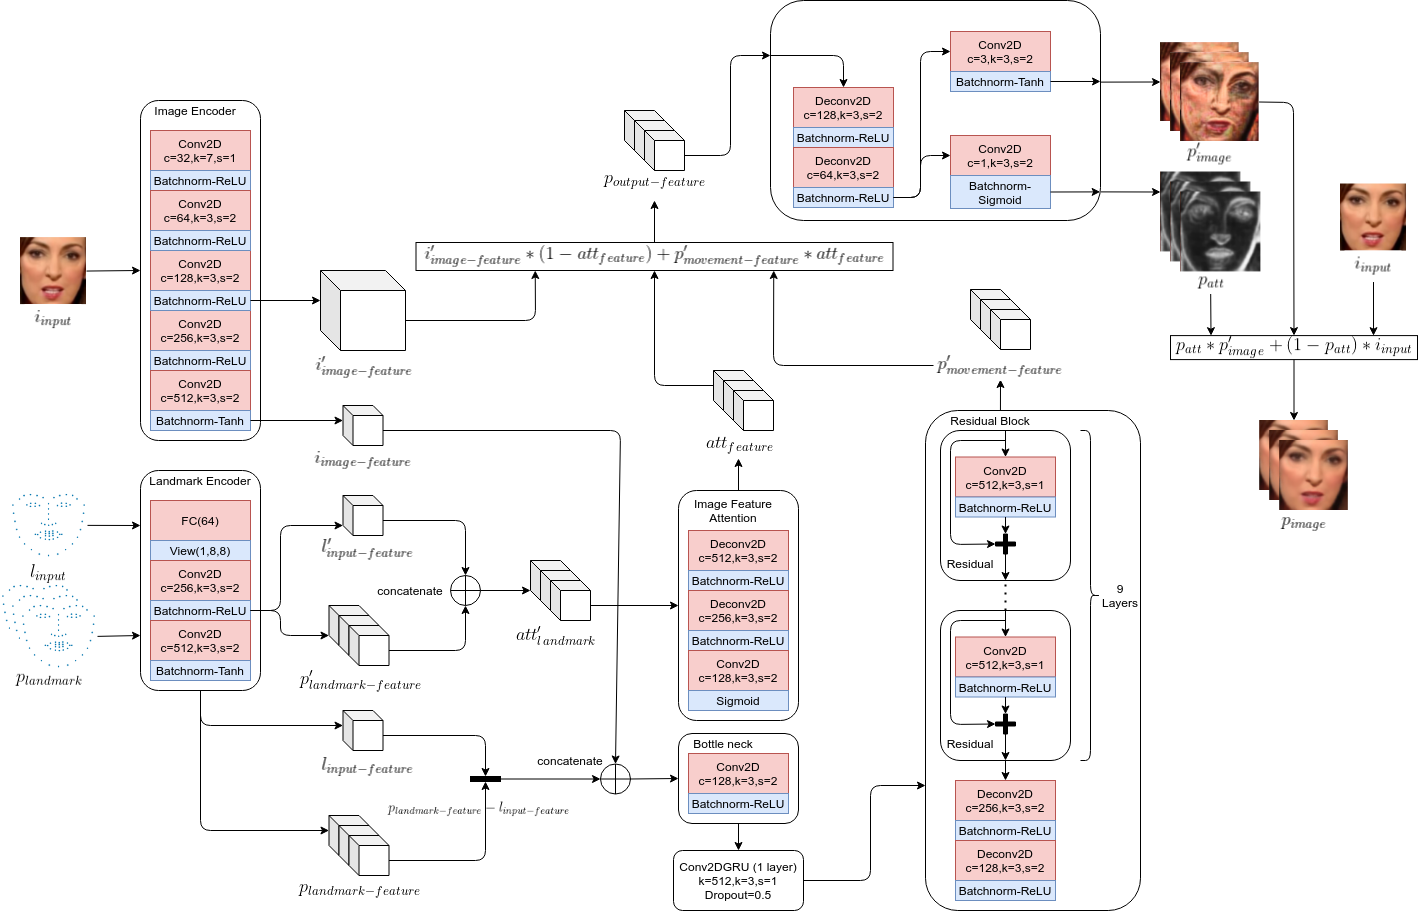
\includegraphics[width=15cm]{./content/materials/generator.png}
    \caption{Cấu trúc của bộ giải mã landmark của khuôn mặt (Generator)}
\end{figure}

\subsection{Cấu trúc của bộ phân biệt hình ảnh (Discriminator)}

\begin{figure}[H]
    \centering
    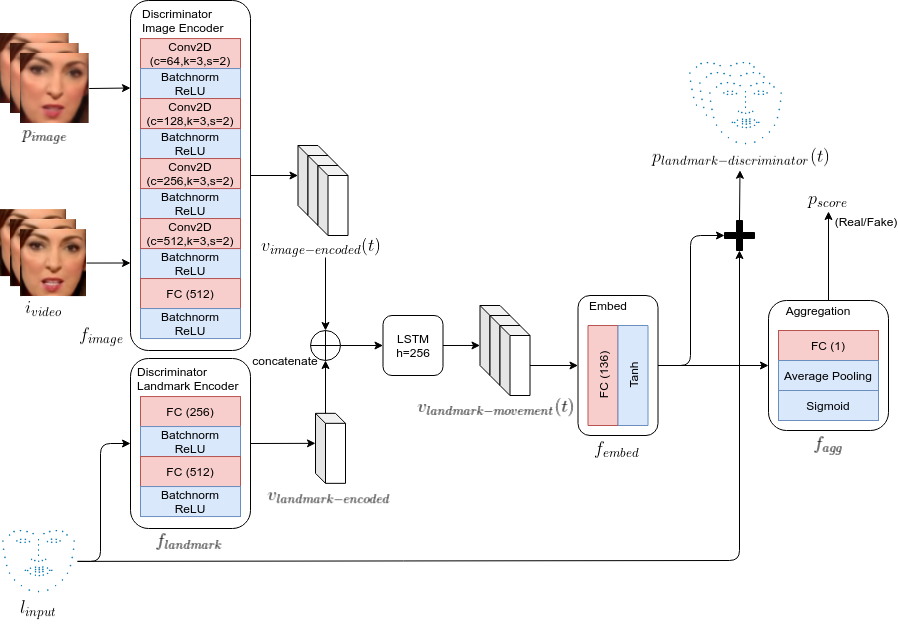
\includegraphics[width=15cm]{./content/materials/discriminator.png}
    \caption{Cấu trúc của bộ phân biệt hình ảnh (Discriminator)}
\end{figure}

\subsection{Hàm mất mát được sử dụng cho hệ Generator - Discriminator}

\section{\texorpdfstring{Kết quả nghiên cứu}{result}}
%Mô tả ngắn gọn các kết quả nghiên cứu, thực nghiệm. Bàn luận về điểm mạnh, điểm yếu của mô hình được xây dựng trong luận văn. So sánh kết quả thu được trong quá trình nghiên cứu, thực nghiệm của đề tài và đối chiếu với kết quả nghiên cứu, thực nghiệm của các tác giả khác một cách khách quan. Nêu lên điểm nổi bật, khác biệt của luận văn đối với các nghiên cứu khác.

Trong phần này, tất cả các mô hình được miêu tả đều được huấn luyện trên thiết bị đồ họa NVIDIA V100 và bộ xử lý Intel Xeon với 24GB bộ nhớ truy xuất ngẫu nhiên. Các thí nghiệm tạo sinh hình ảnh và đanh giá dữ liệu đều được thực hiện trên thiết bị máy tính cá nhân sử dụng thiết bị đồ họa RTX 3070, bộ xử lý Intel Core I5 8600K và 32GB bộ nhớ truy xuất ngẫu nhiên.

\subsection{Các kết quả trên tập dữ liệu GRID}

\begin{table}[h]
    \centering
    \begin{tabular}{c | c | c | c | c}
    \hline 
    \multicolumn{5}{c}{GRID}\\
    \hline 
    \textbf{$\mathcal{L}_{landmark}$} & \textbf{$\mathcal{L}_{pix}$} & \textbf{$\mathcal{L}_{gans-dis}$} & \textbf{$\mathcal{L}_{gans-landmark}$} & \textbf{$\mathcal{L}$}\\
    \hline
    $4.9200 \times 10^{-4}$ & $4.1575 \times 10^{-2}$ & $0.9964$ & $7.6990 \times 10^{-2}$ & $1.4892$\\
    \end{tabular}
    \caption{Các giá trị mất mát của mạng khi hội tụ tại vòng lặp thứ 8}
    \label{table:grid_loss}
\end{table}

\begin{figure}[H]
    \centering
    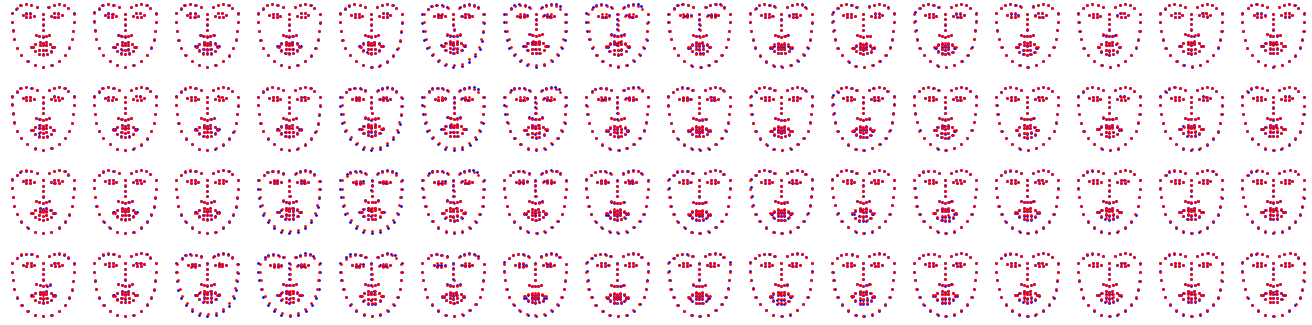
\includegraphics[width=15cm]{./content/materials/grid_examples-landmark.png}
    \caption{Kết quả tạo sinh cột mốc gương mặt trên tập GRID}
\end{figure}

\begin{figure}[H]
    \centering
    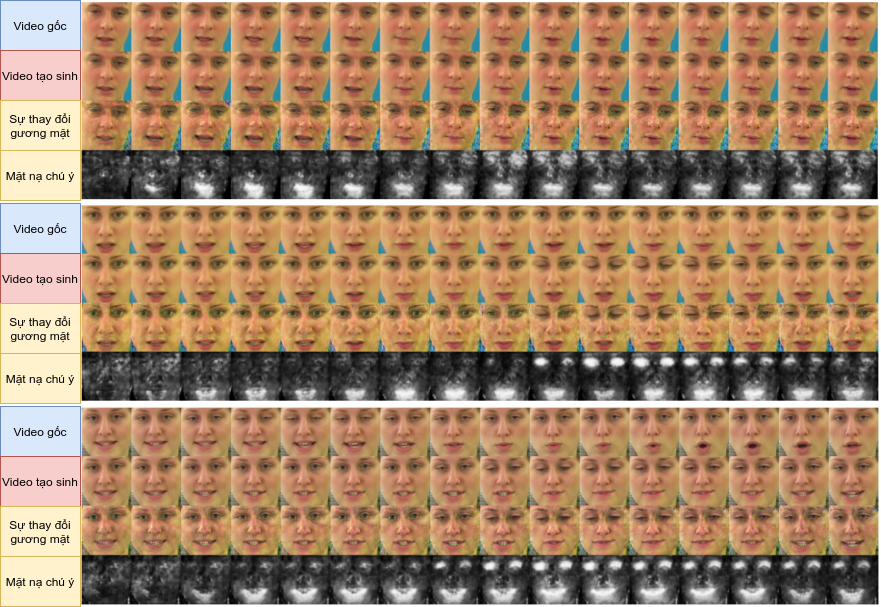
\includegraphics[width=15cm]{./content/materials/grid_examples-face.png}
    \caption{Kết quả tạo sinh gương mặt theo giọng nói trên tập GRID}
\end{figure}

\subsection{Các kết quả trên tập dữ liệu LRW}

Do tập dữ liệu có khối lượng dữ liệu lớn hơn tập GRID nhiều lần và dữ liệu không được chuẩn hóa tốt như tập dữ liệu GRID. Huấn luyện mạng trên tập LRW cũng khó hội tụ hơn và không cho kết quả tốt như tập GRID. Với tập dữ liệu LRW, thời gian huấn luyện là 9 giờ 30 phút cho mỗi vòng lặp qua dữ liệu (tính trên thiết bị đồ họa NVIDIA V100). Mạng hội tụ và cho kết quả tốt nhất sau 25 vòng lặp. Tại thời điểm hội tụ, các hàm mất mát trên mạng có giá trị:

\begin{table}[h]
    \centering
    \begin{tabular}{c | c | c | c}
    \hline 
    \multicolumn{4}{c}{LRW}\\
    \hline 
    \textbf{$\mathcal{L}_{pix}$} & \textbf{$\mathcal{L}_{gans-dis}$} & \textbf{$\mathcal{L}_{gans-landmark}$} & \textbf{$\mathcal{L}$}\\
    \hline
    $6.8502 \times 10^{-2}$ & $0.6931$ & $5.2412 \times 10^{-2}$ & $1.4306$\\
    \end{tabular}
    \caption{Các giá trị mất mát của mạng khi hội tụ tại vòng lặp thứ 25}
    \label{table:lrw_loss}
\end{table}

\begin{figure}[H]
    \centering
    \includegraphics[width=15cm]{./content/materials/lrw_examples-landmark.png}
    \caption{Kết quả tạo sinh cột mốc gương mặt trên tập LRW}
\end{figure}

Hình sau thể hiện kết quả tạo sinh video khi cho mô hình tạo sinh ảnh trên tập kiểm thử với 3 trường hợp: ảnh mẫu được chuẩn hóa tốt, ảnh đầu vào bị lệch, và ảnh đầu vào được quay một bên mặt.

\begin{figure}[H]
    \centering
    \includegraphics[width=15cm]{./content/materials/lrw_examples-frontal.png}
    \caption{Kết quả tạo sinh gương mặt theo giọng nói trên tập LRW, trường hợp ảnh đầu vào là hình ảnh chiếu thẳng mặt người nói, mặt người được canh bốn góc, mũi nằm ở giữa khung hình}
\end{figure}

\begin{figure}[H]
    \centering
    \includegraphics[width=15cm]{./content/materials/lrw_examples-miss_aligned.png}
    \caption{Kết quả tạo sinh gương mặt theo giọng nói trên tập LRW, trường hợp ảnh đầu vào là hình ảnh bị lệch, mặt người nằm ở 1 phía trên khung hình}
\end{figure}

\begin{figure}[H]
    \centering
    \includegraphics[width=15cm]{./content/materials/lrw_examples-half_face.png}
    \caption{Kết quả tạo sinh gương mặt theo giọng nói trên tập LRW, trường hợp ảnh đầu vào là hình ảnh lệch hẳn về một bên mặt}
\end{figure}

Hình ảnh trên cho thấy, mạng cho kết quả tốt nhất khi tạo sinh ảnh có chứa mặt người mẫu được chụp theo hướng chính diện, mặt người được chuẩn hóa tốt.

\section{\texorpdfstring{Kết luận và hướng nghiên cứu mở rộng đề tài}{conclusion}}
%Mô tả, bình luận ngắn gọn và đưa ra kết luận về kết quả nghiên cứu của luận văn và cách thức áp dụng thực tiễn. Đề ra các hướng nghiên cứu mở rộng cho Luận văn.



% \section{\texorpdfstring{Giới thiệu đề tài}{Introduce}}
Bài toán tạo sinh dữ liệu dựa trên những nguồn dữ liệu có tính chất khác nhau đã và đang trở thành xu thế trong những năm trở lại đây. Đây là bài toán có tính cấp bách, mang lại giá trị cao về mặt kiến thức cho ngành trí tuệ nhân tạo nói riêng và giá trị về mặt kinh tế, công nghệ chung cho toàn xã hội xã hội. Bên cạnh đó, việc tạo sinh dữ liệu về con người đã đạt được những tiến bộ vượt bậc, đặc biệt là tạo sinh dữ liệu hình ảnh khuôn mặt người. Trong để tài này, mục đích nghiên cứu là: cho biết một vài dữ liệu về gương mặt của một người bất kỳ (hình ảnh, video ngắn) và một đoạn tiếng nói bất kỳ, tạo sinh hình ảnh khuôn mặt người đó đang nói đoạn tiếng nói đã cho một cách chân thực.

Ý nghĩa khoa học: Đóng góp cho sự phát triển chung của xu hướng tạo sinh dữ liệu mới dựa trên các tính chất của dữ liệu ban đầu. Việc tìm ra phương pháp giải quyết tốt bài toán sẽ tạo nên tảng để giải quyết những bài toán xa hơn, phức tạp hơn như: tạo sinh nửa người trên, tạo sinh toàn bộ cơ thể người, hay tạo sinh cả một bối cảnh trong phim. Đề tài giúp hiện thực, cải tiến các phương pháp hiện có trong các bài nghiên cứu gần đây, so sánh và cải tiến để cho ra kết quả tạo sinh tốt hơn, đóng góp thêm phương pháp mới cho việc tạo sinh ảnh. Đồng thời, các phương pháp tạo sinh dữ liệu cũng giúp làm giàu dữ liệu để huấn luyện, kiểm thử cho các mô hình học máy, học sâu khác.

Ý nghĩa thực tiễn: Giải quyết thành công vấn đề này đem lại giá trị to lớn về mặt công nghệ, kinh tế và xã hội. Chúng ta có thể tái hiện lại gương mặt người đang nói ở nhiều thứ tiếng khác nhau, tạo sinh khuôn mặt người đại diện trong các hội nghị trực tuyến, tích hợp vào các trò chơi điện tử để làm chúng trở nên chân thực hơn, truyền video trong điều kiện băng thông giới hạn, giả lập trợ lý ảo có hình dáng con người,... Đối với ngành truyền thông, nó có thể tạo ra biên tập viên ảo. Đối với ngành điện ảnh, giải trí, sáng tạo nội dung nó cũng có giá trị ứng dụng khi giúp giảm bớt áp lực lên khâu hóa trang, kỹ xảo.

Kiến trúc mạng Generative Adversarial Network \cite{gans_base} ra đời vào năm 2014 đã đánh dấu một bước chuyển mình mới cho ngành trí tuệ nhân tạo. Kiến trúc này giúp cho việc tạo sinh dữ liệu được thực hiện một cách hiệu quả và chính xác hơn. Dựa trên nền tảng đó, các nghiên cứu về việc tạo sinh ảnh gương mặt người cũng được tiến hành và ngày càng có những bước tiến mới. 

Để tạo sinh mặt người đang nói, các công trình nghiên cứu tập trung chủ yếu vào vùng miệng. Bài nghiên cứu vào năm 2018 của Lele Chen \cite{chen2018} đưa ra phương pháp tạo sinh video vùng miệng của người đang nói với đầu vào là ảnh tĩnh của khuôn miệng và một đoạn âm thanh có chứa tiếng nói. Vào năm 2019, Lele Chen \cite{chen2019} và Vougioukas \cite{vougioukas2019} tiếp tục đưa ra phương pháp tạo sinh cả khuôn mặt người dựa vào ảnh tĩnh của khuôn mặt và đoạn âm thanh chứa tiếng nói. Năm 2020, Vougioukas \cite{vougioukas2020} đã cải tiến phương pháp tạo sinh mặt và cập nhật thêm hành động chớp mắt, Lele Chen \cite{chen2020} cũng đưa ra phương pháp mới để tạo sinh mặt hiệu quả hơn, tự nhiên hơn với việc di chuyển của vùng đầu trên khung hình.

Nhìn chung, các nghiên cứu này đã đưa ra các kiến trúc mạng hiệu quả để tạo sinh khuôn mặt cũng như các phương pháp, lập luận và chứng minh tính hiệu quả của các kiến trúc mạng được đề xuất. Mặc dù các thông số của thử nghiệm đưa ra là khá tốt, các nghiên cứu của Vougioukas vẫn chưa thể tạo ra chuyển động của đầu, kết quả tạo sinh của Vougioukas đôi khi không giữ được đặc trưng của ảnh. Nghiên cứu của Lele Chen năm 2020 \cite{chen2020} đã tạo ra chuyển động cho phần đầu dựa trên tiếng nói, nhưng khuôn mặt được tạo sinh vẫn còn có thể bị nhận ra qua các phép thử Turing, và chuyển động của đầu đôi khi vẫn chưa được tự nhiên, mạng cũng có cấu trúc rất phức tạp và đòi hỏi nhiều tài nguyên tính toán để có thể huấn luyện.

% \chapter{Tổng quan tình hình nghiên cứu}
% Sơ lược, phân tích, đánh giá các công trình nghiên cứu nổi tiếng có liên quan đến đề tài. Nêu những vấn đề bức thiết cần phải giải quyết, chỉ ra những thiếu sót mà những nghiên cứu trước đây chưa giải quyết được.

\section{Bài nghiên cứu "Lip Movements Generation at a Glance"\cite{chen2018}}

\begin{figure}[H]
    \centering
    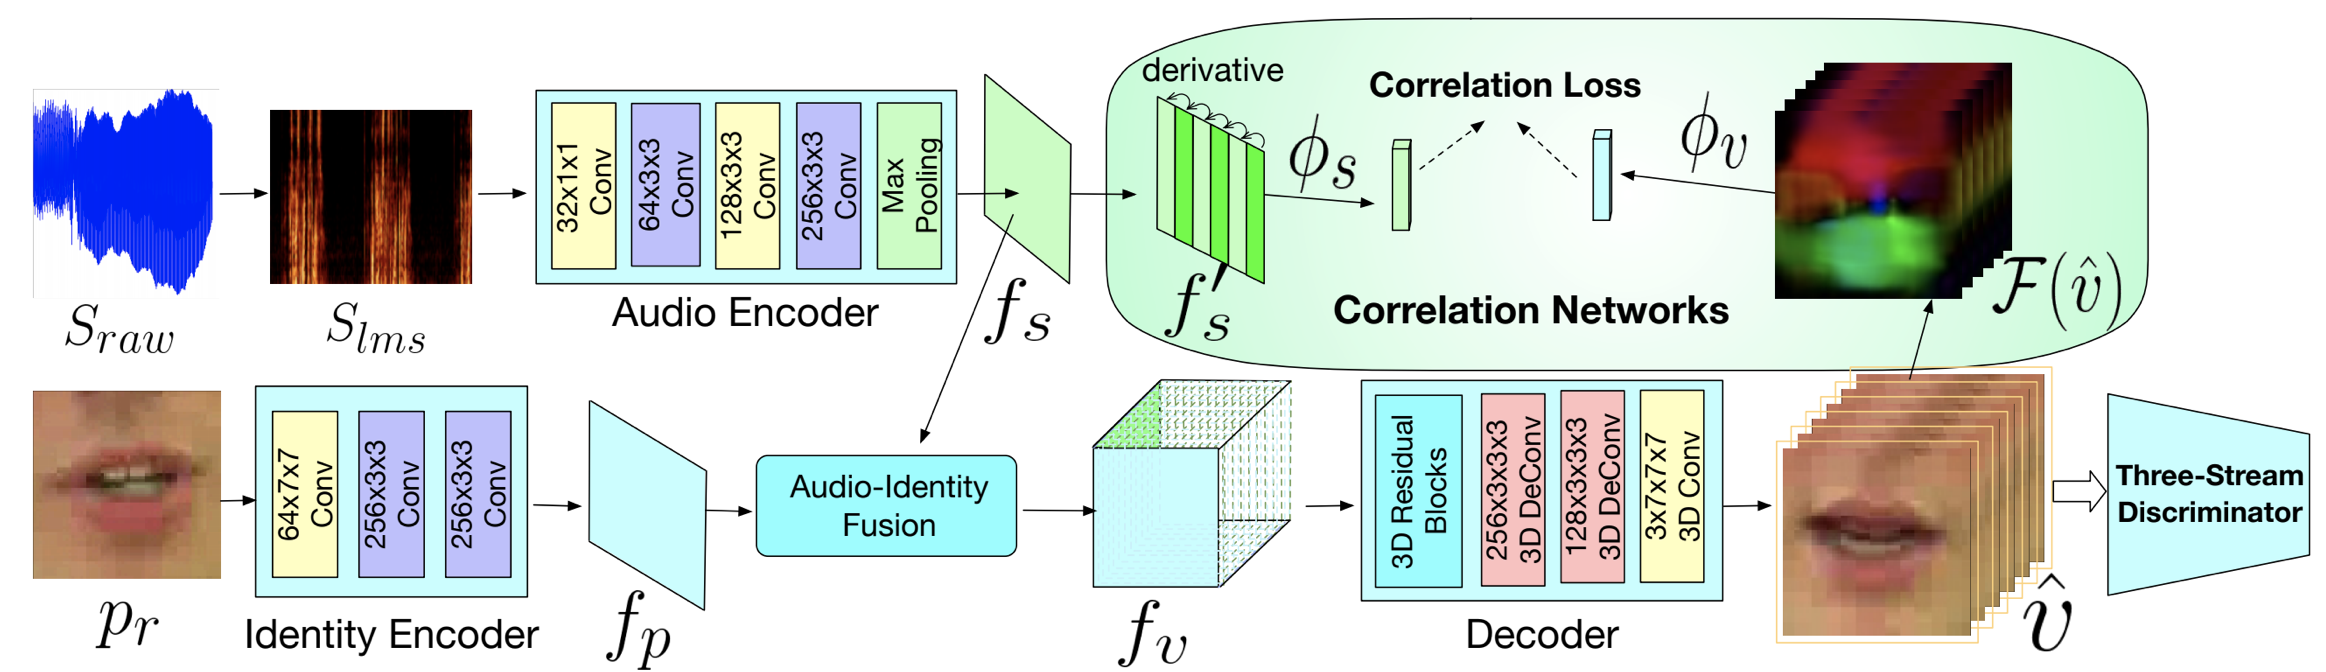
\includegraphics[width=15cm]{./content/images/chen2018_model.png}
    \caption{Mô hình của bài báo Lip Movements Generation at a Glance}
    \label{fig:chen2018_model}
\end{figure}

Việc tạo sinh khẩu hình miệng khớp với tiếng nói là bước đầu tiên để thực hiện việc tạo sinh khuôn mặt. Nghiên cứu này đã thành công trong việc tạo sinh khẩu hình miệng từ một ảnh tĩnh chứa hình ảnh khuôn miệng của một người bất kỳ, và một đoạn âm thanh chứa tiếng nói. Bằng phương pháp kết hợp các đặc trưng âm thanh và hình ảnh, nghiên cứu cho ra kết quả tốt và có độ chính xác cao hơn so với các nghiên cứu trước đó. Hình \ref{fig:chen2018_model} mô tả cấu trúc của mạng tạo sinh ảnh được dùng. Đầu tiên, âm thanh được cắt thành các đoạn nhỏ dài 0.64s, các đoạn này được chuyển thành phổ Log-Mel ($S_{raw}$ thành $S_{lms}$), sau đó qua một bộ Audio Encoder để trích đặc trưng, ta có đặc trưng âm thanh $f_s$ là một ma trận 2 chiều kích thước $F \times T$. Bên cạnh đó, hình ảnh khuôn miệng cũng được đưa qua một bộ Identity Encoder để tạo thành ma trận 2 chiều $f_p$ kích thước $H \times W$.

\begin{figure}[H]
    \centering
    \begin{minipage}{0.48\textwidth}
        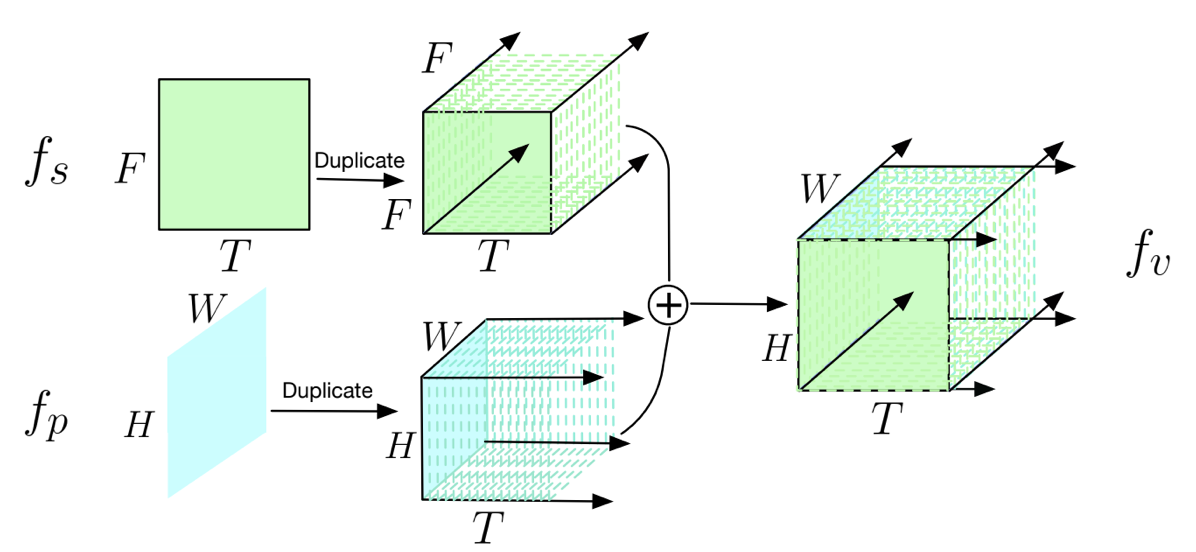
\includegraphics[width=7cm]{./content/images/chen2018_fusion.png}
        \caption{Phương pháp kết hợp đặc trưng hình ảnh và âm thanh}
        \label{fig:chen2018_fusion}
    \end{minipage}\hfill
    \begin{minipage}{0.48\textwidth}
        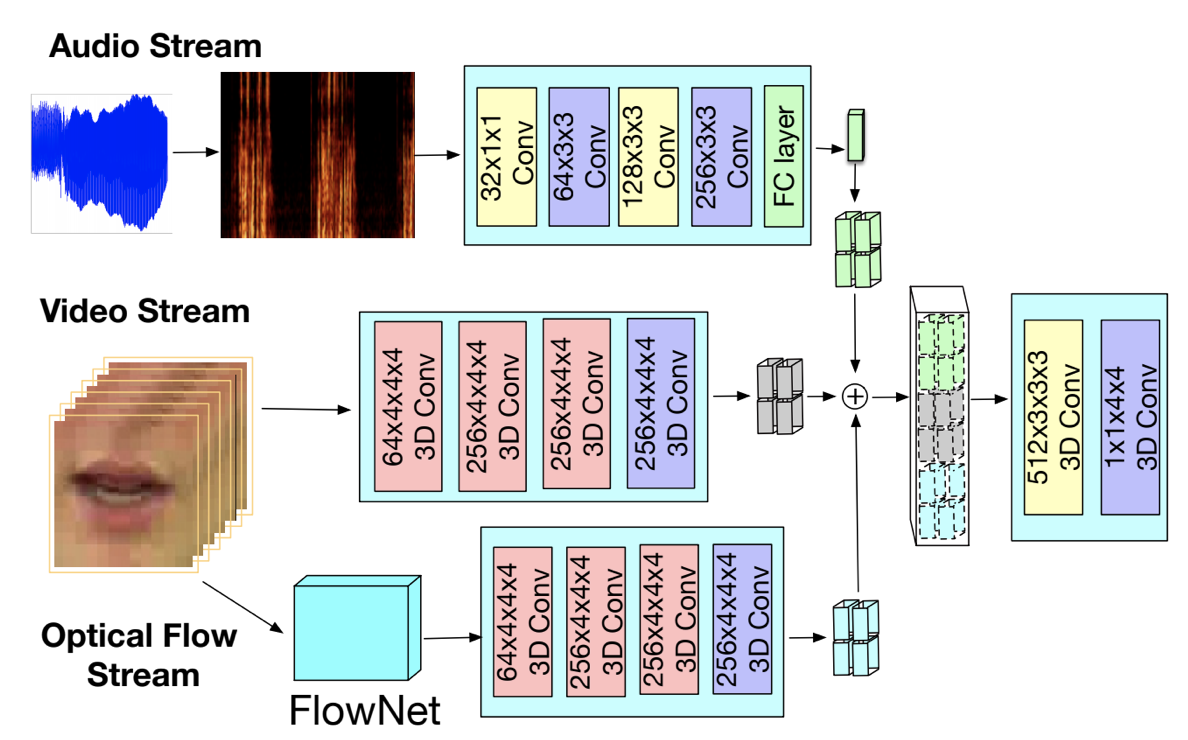
\includegraphics[width=7cm]{./content/images/chen2018_gans.png}
        \caption{GANs Discriminator với 3 loại đặc trưng}
        \label{fig:chen2018_gans}
    \end{minipage}
\end{figure}

Để kết hợp hai đặc trưng hình ảnh, âm thanh với nhau để tạo sinh hình ảnh mới, tác giả bài báo đề xuất phương pháp nhân bản ma trận $f_s$ F lần và nhân bản ma trận $f_p$ T lần thành hai tensor ba chiều, sau đó nối tiếp các kênh của hai tensor này để tạo thành khối tensor ba chiều mới. Để có thể nối tiếp được với nhau, Tác giả đã đặt các thông số $H = W = F$. Hình \ref{fig:chen2018_fusion} miêu tả cách kết hợp hai đặc trưng hình ảnh - âm thanh thành khối đặc trưng chung $f_v$, khối $f_v$ có kích thước $W \times H \times T$. Khối đặc trưng này sau cùng được chuyển đổi thành ảnh đầu ra $\hat{v}$ nhờ vào mạng Decoder. Mạng Decoder này sử dụng kiến trúc 3D Residual và các khối Deconvolution nhằm bảo toàn các đặc điểm của hình ảnh gốc.

Đồng thời, nghiên cứu này cũng chỉ ra rằng đặc tính của khuôn miệng trong video là hình ảnh thường đi trước âm thanh, và độ trễ âm thanh - hình ảnh là không đồng nhất trong các video khác nhau. Vì vậy, để tạo sinh một video chân thực, ta phải quan tâm đến độ trễ này. Khối Correlation Network trong hình \ref{fig:chen2018_model} miêu tả cách tính toán giá trị Corelation Loss. Để tính giá trị này, bộ tính toán cần có một encoder ($\phi_s$) để encode sự thay đổi của âm thanh và một encoder ($\phi_v$) để encode sự thay đổi của hình ảnh. Ma trận $f_s$ được tính đạo hàm theo trục T thành $f'_s$, hình ảnh được tạo sinh $\hat{v}$ cũng được đưa qua hàm $\mathcal{F}$ để lấy đặc trưng Optical Flow. Sau đó, cả hai đặc trưng thể hiện sự thay đổi của âm thanh và hình ảnh theo thời gian này được đưa qua các encoder $\phi_s$ và $\phi_v$ để tạo ra hai vector có cùng số chiều. Công thức tính của giá trị Correlation Loss chính là hiệu của 1 và giá trị cosin giữa hai vector đặc trưng cuối cùng:

\begin{equation}
    \ell_{corr} = 1 - \frac{\phi_s(f'_s)\cdot\phi_v(\mathcal{F}(v))}{\|\phi_s(f'_s)\|_2\cdot\|\phi_v(\mathcal{F}(v))\|_2}
    \label{eqn:chen2018_corr_loss}
\end{equation}


Cấu trúc mạng GANs cũng đã được sử dụng trong nghiên cứu này nhằm mục đích tạo ra chuyển động mượt mà cho chuỗi hình ảnh trong video và làm cho chất lượng ảnh tạo sinh tốt hơn. Bộ phân biệt (Discriminator) giữa ảnh thật và ảnh tạo sinh ($D$) được miêu tả trong hình \ref{fig:chen2018_gans}. Đặc trưng Log-Mel của âm thanh được encode thành một vector bằng một mạng Convolution - Fully connected, sau đó vector này được nhân bản và ghép nối để có số chiều bằng với tensor của hai đặc trưng còn lại. Hình ảnh được đưa vào mạng được encode bởi các khối 3D Convolution để có được tensor đặc trưng ảnh. Các ảnh này cũng được đưa qua mạng FlowNet để đưa ra đặc trưng Optical Flow, đặc trưng này cũng được encode để tạo ra tensor đặc trưng cho chuyển động trong video. Sau cùng, ba đặc trưng này được ghép nối tiếp theo kênh và được đưa qua các khối 3D Convolution để lấy được xác suất dự đoán ảnh thật hay tạo sinh của mạng. Cặp video - âm thanh đưa vào mạng có thể là video thật và đoạn âm thanh khớp với video đó, hoặc video thật và một đoạn âm thanh khác, hoặc video được tạo sinh và đoạn âm thanh tương ứng tạo ra nó. Hàm mất mát của mạng được định nghĩa như sau:

\begin{equation}
    \ell_{dis} = -logD([s^j, v^j]) - \lambda_plog(1 - D([s^j, \hat{v}])) - \lambda_ulog(1 - D([s^j, v^k])), k \ne j
\end{equation}

Để so sánh sự tương đồng về mặt tổng quan giữa hai video (video thật và video được tạo sinh), tác giả sử dụng một bộ Autoencoder. Bộ Autoencoder này được huấn luyện độc lập với mạng chính và sử dụng cùng bộ dữ liệu với mạng chính. Phần encoder ($\varphi$) được giữ lại để encode hình ảnh từ video nhằm mục đích trích xuất đặc trưng của chuỗi hình ảnh. Hàm Perceptual Loss $\ell_{perc}(\hat{v}, v)$ được dùng để tính toán độ sai lệch về mặt tổng quan giữa video được tạo sinh từ tiếng nói và video thật tương ứng với tiếng nói:
\begin{equation}
    \ell_{perc}(\hat{v}, v) = \|\varphi(v) - \varphi(\hat{v})\|^2_2
    \label{eqn:chen2018_perc_loss}
\end{equation}

Hàm mất mát của cuối cùng của mạng được định nghĩa:
\begin{equation}
    \mathcal{L} = \ell_{corr} + \lambda_1\ell_{pix} + \lambda_2\ell_{perc} + \lambda_3\ell_{gen}
    \label{eqn:chen2018_loss}
\end{equation}

Trong đó:
\begin{itemize}
\item $\ell_{corr}$: Là giá trị mất mát do sự sai lệch giữa hình ảnh và âm thanh đã nêu ở (\ref{eqn:chen2018_corr_loss}).
\item $\ell_{pix}$: Giá trị mất mát dựa trên sự sai khác ở cấp độ điểm ảnh giữa ảnh được tạo sinh và ảnh trong video thật, $\ell_{pix} = \|v-\hat{v}\|$.
\item $\ell_{perc}$: Giá trị mất mát đo độ sai khác trên toàn bộ chuỗi hình ảnh (đã nêu ở (\ref{eqn:chen2018_perc_loss})).
\item $\ell_{gen}$: Giá trị mất mát của bộ tạo sinh ảnh dựa trên hàm phân biệt $D$: $\ell_{gen} = -logD([s^j, \hat{v}^j])$.
\end{itemize}

Mô hình được huấn luyện và kiểm thử trên các tập dữ liệu GRID, LDC và LRW. Kết quả kiểm thử cho thấy mô hình này cho kết quả tạo sinh hình ảnh tốt hơn hẳn so với các nghiên cứu trước đó. Các độ đo PSNR, SSIM, LMD và CPBD được sử dụng để kiểm chứng. Sau đây là kết quả được khảo sát bới tác giả:

\begin{figure}[H]
    \centering
    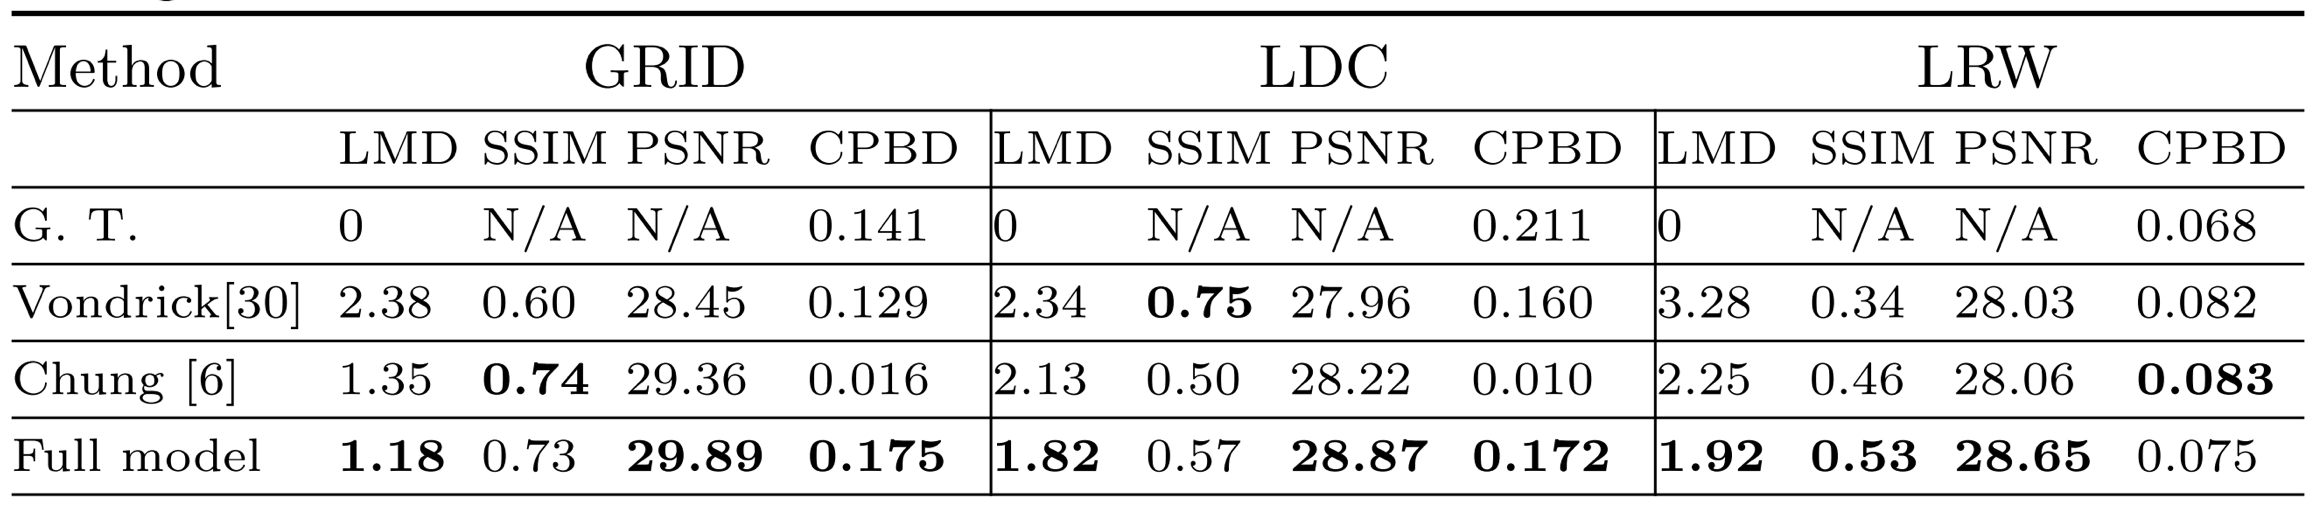
\includegraphics[width=15cm]{./content/images/chen2018_result.png}
    \caption{Kết quả đánh giá và so sánh mô hình trong nghiên cứu Lip Movements Generation at a Glance}
    \label{fig:chen2018_result}
\end{figure}

Nghiên cứu này đã đưa ra các phương pháp phù hợp và tiến bộ để trích xuất và kết hợp đặc trưng hình ảnh và âm thanh, đồng thời cũng tận dụng phương pháp GANs để cải thiện chất lượng của ảnh được tạo sinh. Độ hiệu quả của cấu trúc mạng được thể hiện qua kết quả đo lường vượt trội so với các nghiên cứu cùng thời điểm. Tuy nhiên, cấu trúc mạng này có một số yếu điểm. Thứ nhất, mạng chỉ có thể nhận vào hình ảnh tĩnh và một đoạn âm thanh có độ dài xác định (0.64s) và cho ra số khung hình tương ứng với khoảng thời gian đó (16 khung hình). Thứ hai, tác giả vẫn chưa chú ý đến hiện tượng nhảy hình của video được tạo sinh, mạng không có cơ chế để đảm bảo việc chuyển ảnh mượt mà, ít sai khác về độ tương phản, ánh sáng, màu sắc giữa các khung ảnh gần nhau.

%------------------------------------------------------------------------

\section{Bài nghiên cứu "End-to-End Speech-Driven Facial Animation with Temporal GANs"\cite{vougioukas2019}}
\label{sec:vougioukas2019}

\begin{figure}[H]
    \centering
    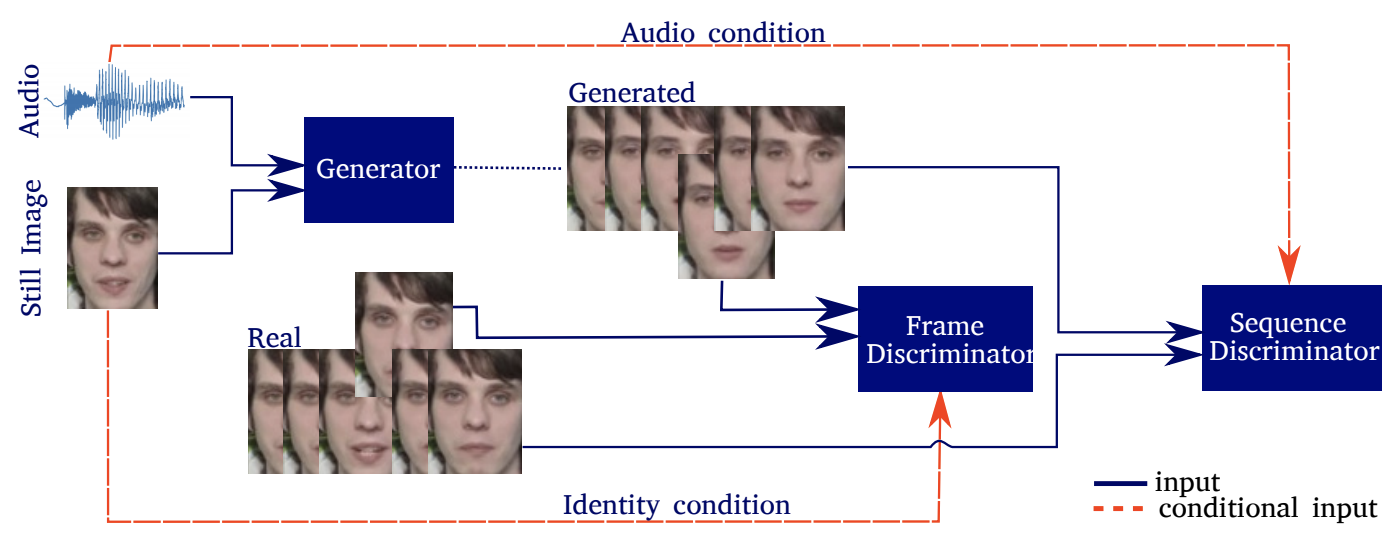
\includegraphics[width=15cm]{./content/images/vou2019_model.png}
    \caption{Mô hình của nghiên cứu End-to-End Speech-Driven Facial Animation with Temporal GANs}
    \label{fig:vou2019_model}
\end{figure}

Nghiên cứu của Vougioukas vào năm 2019 có mục tiêu là tạo ra chuỗi hình ảnh của toàn bộ gương mặt người đang nói với đầu vào là một ảnh tĩnh chứa mặt người bất kỳ và một đoạn tiếng nói bất kỳ. Kiến trúc của mạng được miêu tả trong hình \ref{fig:vou2019_model}, được bao gồm ba phần chính. Bộ tạo sinh ảnh Generator nhận vào một đoạn âm thanh tiếng nói có độ dài bất kỳ và một ảnh tĩnh, sử dụng những dữ liệu này như một gợi ý để tạo sinh chuỗi hình ảnh mới với mặt người đang nói tiếng nói tương ứng. Bộ phân biệt ảnh theo khung hình Frame Discriminator cũng nhận vào ảnh tĩnh nói trên, đồng thời nhận thêm một ảnh khác, ảnh này hoặc được tạo sinh từ Generator, hoặc được trích xuất từ video trong bộ dữ liệu. Frame Discriminator sẽ được huấn luyện để phân biệt đâu là ảnh được tạo sinh và đâu là ảnh thật được trích xuất từ video huấn luyện. Bộ phân biệt chuỗi ảnh Sequence Discriminator nhận vào đoạn tiếng nói và một chuỗi hình ảnh trong video. Chuỗi hình ảnh này có thể là hình ảnh được tạo sinh hoặc hình ảnh gốc từ video tương ứng. Bộ Sequence Discriminator sẽ học cách phân biệt hai loại video này trong quá trình huấn luyện. Theo như cơ chế GANs, trong quá trình huấn luyện, hàm mất mát của hai bộ Discriminator sẽ tạo ra lan truyền ngược và cập nhật trọng số của chính nó và của cả Generator. Từ đó, cả ba mạng này đều sẽ dần trở nên chính xác hơn.

\begin{figure}[H]
    \centering
    \begin{minipage}{0.48\textwidth}
        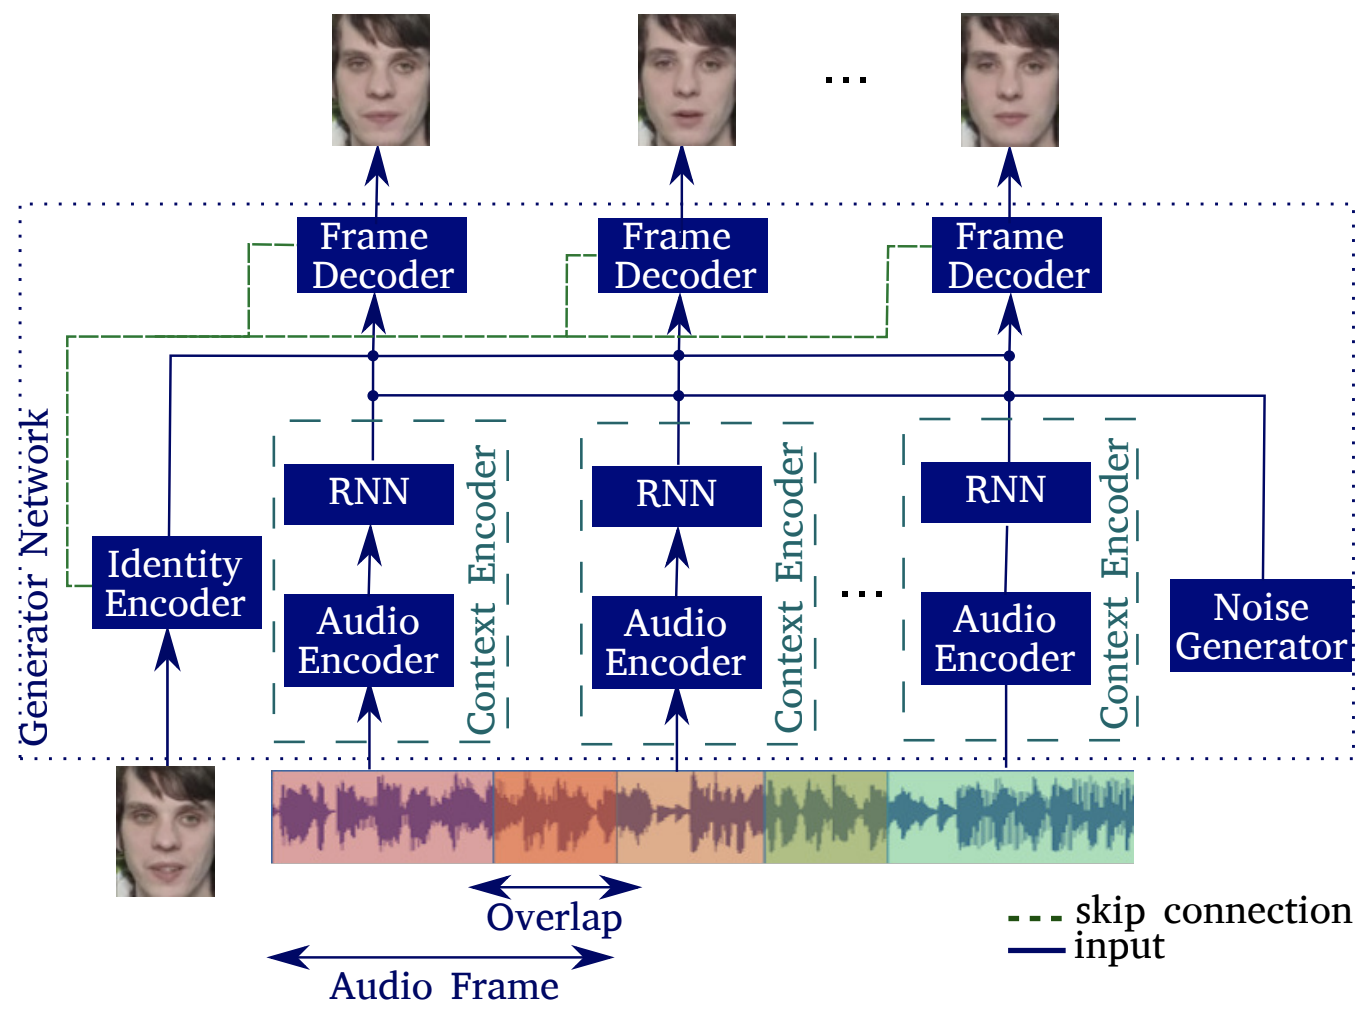
\includegraphics[width=7cm]{./content/images/vou2019_gen.png}
        \caption{Kiến trúc bộ Generator}
        \label{fig:vou2019_gen}
    \end{minipage}\hfill
    \begin{minipage}{0.48\textwidth}
        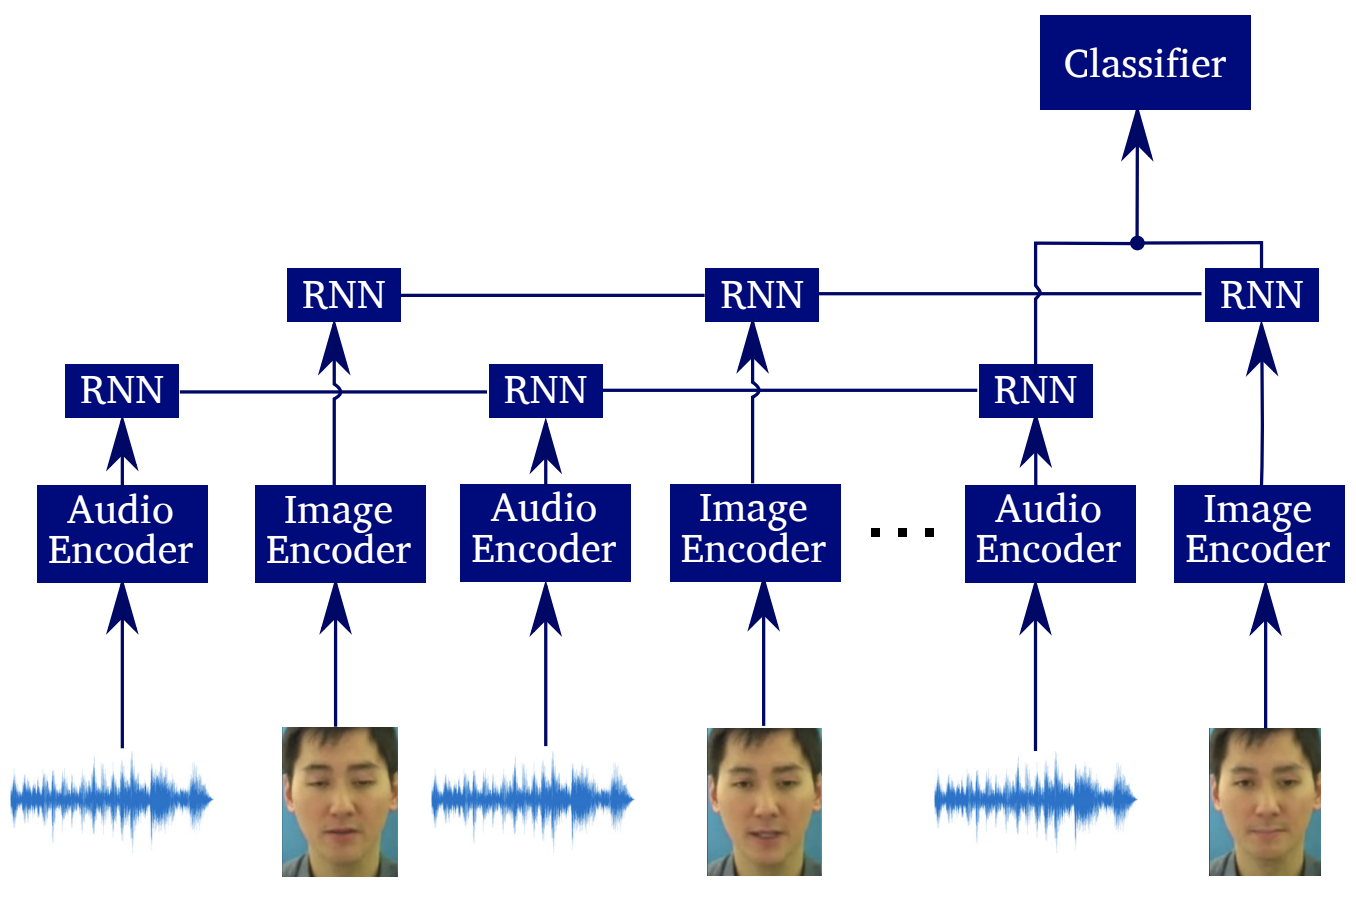
\includegraphics[width=7cm]{./content/images/vou2019_seq_dis.png}
        \caption{Kiến trúc bộ Sequence Discriminator}
        \label{fig:vou2019_seq_dis}
    \end{minipage}
\end{figure}

Trong nghiên cứu này, video huấn luyện được tách riêng thành âm thanh và hình ảnh. Mỗi khung hình kích thước $96\times128$ được cắt ra từ video tương ứng với đoạn âm thanh dài 0.16s, đoạn âm thanh này tạo thành một vector 8000 điểm. Như vậy, dữ liệu được tiền xử lý bằng cách cắt nhỏ video thành khung ảnh và đoạn âm thanh tương ứng với ảnh đó (âm thanh có chồng lấn giữa các ảnh).

Kiến trúc của bộ tạo sinh chuỗi ảnh Generator được miêu tả trong hình \ref{fig:vou2019_gen}. Identity Encoder là bộ encoder ảnh có tính năng trích xuất đặc trưng của ảnh tĩnh được đưa vào mạng. Bộ encoder này gồm 6 lớp 2D Convolution, mỗi lớp kết hợp với Batchnorm và ReLU ở phía sau. Mạng này giúp trích xuất ảnh đầu vào thành vector 50 chiều ($z_{id}$). Context Encoder là tổng hợp của hai bộ bao gồm Audio Encoder và một bộ RNN hai lớp. Audio Encoder sẽ trích xuất đặc trưng từ đoạn âm thanh 8000 điểm (vector 8000 chiều) để tạo ra vector 256 chiều. Đặc trưng này được đưa vào bộ RNN để bổ sung ngữ nghĩa về mặt thời gian. Ngõ ra của bộ Context Encoder là trạng thái ẩn (hidden state) của bộ RNN có số chiều bằng 256 ($z_c$). Generator còn có một bộ Noise Generator, thực chất là một mạng GRU có chức năng tạo ra vector nhiễu Gauss 10 chiều ($z_n$). $z_{id}$, $z_c$ và $z_n$ được ráp nối với nhau theo kênh tương ứng trước khi đưa vào bộ tạo sinh ảnh. Trong khi $z_{id}$ có chức năng giúp Frame Decoder tái tạo chính xác gương mặt của người nói, $z_c$ sẽ mang thông tin về mặt âm thanh, thời gian và hoàn cảnh, giúp tạo ra gợi ý cho mạng để tạo sinh được hình ảnh tương ứng với âm thanh. Đồng thời, $z_n$ tạo ra tính ngẫu nhiên cho mạng, khi đưa cùng một đầu vào, thì sẽ không khi nào mạng cho ra kết quả giống nhau ở hai lần thử. Đồng thời, tính ngẫu nhiên này lại có tính chất phụ thuộc thời gian (do được tạo ra bởi mạng GRU) đem lại cho hình ảnh được tạo sinh các biểu cảm nhỏ như nháy mắt và các chuyển động nhỏ trên mặt một cách liền lạc.

Ở đầu ra, bộ sinh ảnh Frame Decoder được sử dụng để tạo sinh chuỗi ảnh theo thời gian. Vector đặc trưng ẩn có 316 chiều, từ vector đặc trưng này, Frame Decoder sẽ tạo ra hình ảnh có kích thước bằng với hình mẫu ban đầu ($96\times128$). Nhằm bảo toàn nhận dạng của người trong ảnh mẫu, Frame Decoder được thiết kế theo kiến trúc U-Net gồm 6 lớp Convolution tương ứng với Identity Encoder. Các lớp Convolution này nhận thêm các đặc trưng ẩn từ lớp tương ứng của Identity Encoder để hạn chế việc đánh mất nhận dạng của mặt người mẫu do bị ảnh hưởng bởi độ sâu của mạng. Các đặc trưng ẩn đi qua các lớp Deconvolution và cuối cùng tạo ra ảnh tương ứng với âm thanh.

Bộ phân biệt khung ảnh Frame Discriminator trong hình \ref{fig:vou2019_model} là một mạng Convolution 6 lớp, đầu ra của mạng là xác suất ảnh này được cho là ảnh được tạo sinh. Frame Discriminator giúp cho ảnh tạo sinh từ Generator chân thực hơn, khó phân biệt với ảnh từ video gốc hơn. Bộ phân biệt chuỗi ảnh Sequence Discriminator được miêu tả trong hình \ref{fig:vou2019_seq_dis} có cấu trúc trích xuất đặc trưng tương tự như bộ Generator. Sự khác biệt đến từ bộ trích xuất đặc trưng chuỗi ảnh. Chuỗi hình ảnh được đưa qua bộ Image Encoder để trích xuất đặc trưng ảnh và thu nhỏ số chiều dữ liệu. Các ảnh sau khi qua bộ Image Encoder sẽ được đưa vào mạng RNN hai lớp để cập nhật trạng thái ẩn của mạng RNN. Khi kết thúc chuỗi hình ảnh và âm thanh tương ứng với nó, trạng thái ẩn của hai mạng RNN cho âm thanh và RNN cho hình ảnh được ghép nối tiếp vào nhau theo kênh. Lúc này, đặc trưng âm thanh giúp làm điều kiện để phân biệt chuỗi ảnh tốt hơn. Một bộ Classifier được sử dụng để tính toán xác suất chuỗi ảnh được đưa vào có phải chuỗi được tạo sinh hay không. Bộ Sequence Discriminator giúp cho video tạo ra có sự chân thật trong các chuyển động của khuôn mặt, cũng như sự chân thật trong sự chuyển tiếp giữa các khung hình, nhờ đó tránh được hiện tượng nhảy hình bất thường.

Trong quá trình huấn luyện, các ảnh từ video được cho vào Frame Discriminator ($D_{img}$) bằng cách lấy mẫu với xác suất đều qua hàm $S(x)$ trên chuỗi ảnh $x$. Sequence Discriminator ($D_{seq}$) sẽ phân biệt cả chuỗi ảnh $x$ và âm thanh $a$. Hàm mất mát của GANs được biểu diễn như sau:

\begin{equation}
    \begin{split}
    \mathcal{L}_{adv}(D_{img},D_{seq},G) = &\mathrm{E}_{x\sim P_d}[logD_{img}(S(x),x_1)] + \mathrm{E}_{z\sim P_z}[log(1 - D_{img}(S(G(z)), x_1))] + \\
    &\mathrm{E}_{x\sim P_d}[logD_{seq}(x,a)] + \mathrm{E}_{z\sim P_z}[log(1 - D_{seq}(G(z), a))]
    \end{split}
    \label{eqn:vou2019_adv_loss}
\end{equation}

Hàm mất mát L1 cũng được dùng trên một nửa dưới của ảnh để đảm bảo ảnh được tạo sinh có hình ảnh thể hiện chân thật khuôn miệng và khẩu hình miệng phù hợp với lời nói. Hàm mất mát L1 được biểu diễn như sau:

\begin{equation}
    \mathcal{L}_{L1} = \sum_{p\in[0,W]\times[\frac{H}{2},H]}\vert F_p - G_p \vert
    \label{eqn:vou2019_l1_loss}
\end{equation}

Như vậy, mục tiêu của cả hệ thống là giảm thiểu hàm mất mát chung bằng cách điều chỉnh các trọng số của bộ tạo sinh ảnh Generator ($G$) và các bộ phân biệt ảnh Discriminator ($D$). Hàm mục tiêu của mạng được biểu diễn như sau:

\begin{equation}
    \mathrm{arg}\: \underset{G}{\mathrm{min}}\: \underset{D}{\mathrm{max}}\: \mathcal{L}_{adv} + \lambda\mathcal{L}_{L1}
    \label{eqn:vou2019_loss}
\end{equation}

Sau đây là bảng so sánh của tác giả với các thông số PSNR, SSIM, CPBD, WER và một số độ đo khác. Bài nghiên cứu cũng so sánh kết quả của họ với một nghiên cứu trước đó (Baseline):

\begin{figure}[H]
    \centering
    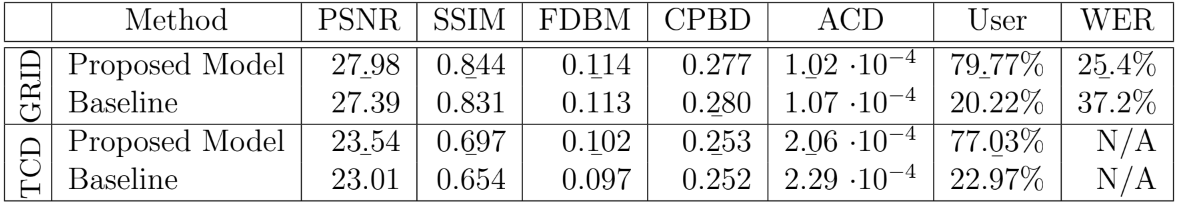
\includegraphics[width=15cm]{./content/images/vou2019_result.png}
    \caption{Kết quả của nghiên cứu End-to-End Speech-Driven Facial Animation with Temporal GANs}
    \label{fig:vou2019_result}
\end{figure}

Mô hình trong bài nghiên cứu đem lại tín hiệu khả quan cho việc tạo sinh ảnh khuôn mặt dựa trên tiếng nói. Phương pháp tạo sinh và các bộ phân biệt ảnh áp dụng phương pháp CGANs một cách hiệu quả nhằm mục đích tạo sự chân thật cho chuỗi ảnh. Một số kết quả được công bố bởi tác giả bài nghiên cứu cho thấy ảnh được tạo sinh có chất lượng tốt, không bị hiện tượng nhảy hình, độ ổn định khung hình tốt, có thể đánh lừa người xem qua phép thử Turing. Theo đó, có tới 79.77\% chuỗi hình ảnh bị đánh nhãn sai (được tạo sinh hay video thật) trên tập dữ liệu GRID và 77.03\% trên tập dữ liệu TCD. Tuy nhiên, một số hạn chế vẫn chưa được giải quyết. Thứ nhất, ngoài vùng miệng, bộ tạo sinh hình ảnh và các bộ phân biệt vẫn chưa chú trọng đến các phần khác trong khuôn mặt nhất là phần nửa trên. Điều này làm cho hình ảnh được tạo sinh thiếu tự nhiên so với video thực tế. Thứ hai, khuôn mặt vẫn chưa thể hiện được cảm xúc tương ứng với tiếng nói. Việc này cũng góp phần làm cho video được tạo sinh dễ bị nhận biết bởi người xem tinh ý. Thứ ba, chuyển động của đầu cũng không được thể hiện trong video làm cho video trở nên cứng nhắc và giả tạo nếu chiếu trong thời gian dài. Thứ tư, sự đồng bộ của tiếng nói và hình ảnh chưa được quan tâm và chưa có cơ chế đảm bảo hình ảnh được tạo sinh sẽ được căn giờ chuẩn xác với âm thanh.

%------------------------------------------------------------------------

\section{Bài nghiên cứu "Realistic Speech-Driven Facial Animation with GANs"\cite{vougioukas2020}}

Đây là bài nghiên cứu có cùng tác giả với bài nghiên cứu trong phần \ref{sec:vougioukas2019}. Với cùng mục tiêu và phương pháp tiếp cận tương đồng với nghiên cứu được công bố  năm 2019, Vougioukas đã có một số cập nhật, bổ sung và đánh giá cho mô hình được xây dựng. Trong nghiên cứu này, Vougioukas đã thêm vào mạng trước đó một bộ phân biệt mới, bộ phân biệt này giúp đảm bảo sự đồng bộ giữa hình ảnh được tạo sinh và tiếng nói tương ứng. Kiến trúc được cập nhật mới thể hiện ở hình \ref{fig:vou2020_model}.

\begin{figure}[H]
    \centering
    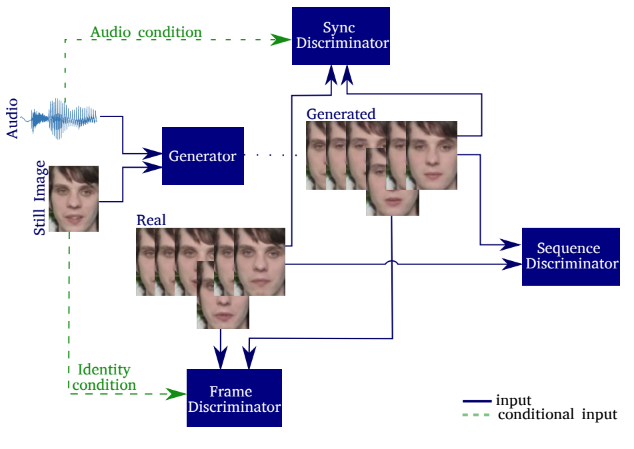
\includegraphics[width=9cm]{./content/images/vou2020_model.png}
    \caption{Kiến trúc mạng được cập nhật trong nghiên cứu mới của Vougioukas}
    \label{fig:vou2020_model}
\end{figure}

Bộ phân biệt tính đồng bộ Sync Discriminator được thể hiện trong hình \ref{fig:vou2020_sync_dis}. Bộ phân biệt này nhận vào một chuỗi hình ảnh nửa dưới (phần ảnh chứa vùng miệng) của mặt người đang nói. Chuỗi hình ảnh này có thể được tạo sinh bởi mạng sinh ảnh Generator hoặc là chuỗi ảnh thật được trích xuất từ video. Đồng thời, mạng cũng nhận vào đoạn tiếng nói tương ứng với chuỗi hình ảnh trên. Dữ liệu đưa vào mạng được thể hiện trong hình \ref{fig:vou2020_sync_input}. Chuỗi hình ảnh được đưa vào gồm 5 ảnh gồm $96 \times 64$ điểm ảnh tạo thành một tensor ba chiều. Tensor này được biến biến đổi thành ma trận hai chiều nhờ một lớp 3D Convolution. Sau đó, ma trận này tiếp tục được trích xuất đặc trưng nhờ ba lớp 2D Convolution và ở cuối là một lớp tuyến tính. Đặc trưng ảnh sau cùng được trích xuất là một vector 256 chiều. Đối với tiếng nói, quy trình trích xuất đặc trưng cũng được áp dụng trên vector âm thanh 8000 chiều. Bộ trích xuất đặc trưng âm thanh được sử dụng bao gồm 5 lớp 1D Convolution và cuối cùng là một lớp tuyến tính. Đặc trưng âm thanh cũng được trích xuất thành một vector 256 chiều. Khoảng cách Euclide giữa hai vector được tính toán theo công thức $d = \Vert \textrm{e}_{\textrm{sm}} - \textrm{e}_{\textrm{a}} \Vert$, với $\textrm{e}_{\textrm{sm}}$ và $\textrm{e}_{\textrm{a}}$ lần lượt là vector đặc trưng chuỗi hình ảnh và vector đặc trưng tiếng nói. Khoảng cách $d$ sau đó được đưa vào một lớp Perceptron để đưa ra sự đo đạc về độ phù hợp giữa chuỗi hình ảnh vùng miệng và âm thanh được đưa vào dưới dạng xác suất.

\begin{figure}[H]
    \centering
    \begin{minipage}{0.48\textwidth}
        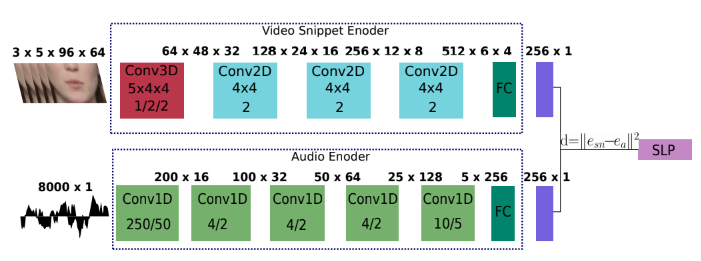
\includegraphics[width=7cm]{./content/images/vou2020_sync_dis.png}
        \caption{Kiến trúc bộ phân biệt đồng bộ Sync Discriminator}
        \label{fig:vou2020_sync_dis}
    \end{minipage}\hfill
    \begin{minipage}{0.48\textwidth}
        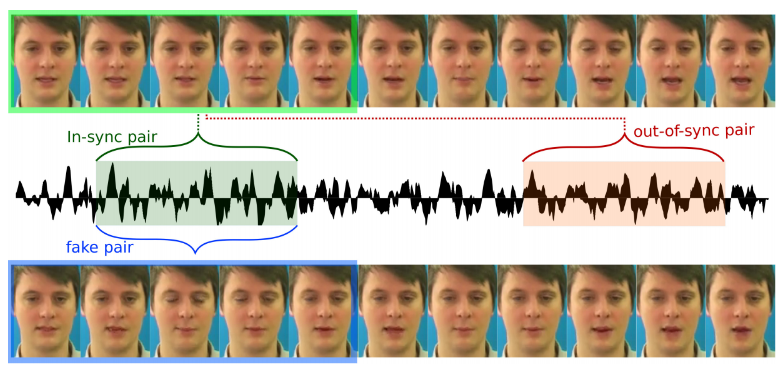
\includegraphics[width=7cm]{./content/images/vou2020_sync_input.png}
        \caption{Miêu tả dữ liệu được đưa vào mạng phân biệt đồng bộ}
        \label{fig:vou2020_sync_input}
    \end{minipage}
\end{figure}

Để có khả năng phân biệt tốt nhất, cặp hình ảnh - tiếng nói được đưa vào mạng được chọn lựa theo ba hoàn cảnh (xem hình \ref{fig:vou2020_sync_input}). Cặp đồng bộ đúng (in-sync pair), là cặp hình ảnh - tiếng nói tương ứng với nhau trong video. Cặp không đồng bộ (out-of-sync pair) gồm hình ảnh được trích xuất từ video nhưng không phù hợp với tiếng nói. Cuối cùng là cặp giả mạo (fake pair) gồm hình ảnh được tạo sinh vào tiếng nói tương ứng tạo sinh ra nó. Nhờ ba cặp này, mạng sẽ học được cách phân biệt sự sai lệch hình ảnh - tiếng nói và đặc biệt là sự đồng bộ của khẩu hình miệng với tiếng nói được cải thiện đáng kể.

Hàm mất mát phân biệt $\mathcal{L}_{adv}$ của mạng cũng được cập nhật thêm hàm mất mát của bộ phân biệt đồng bộ. Qua đó:

\begin{equation}
    \mathcal{L}_{adv} = \lambda_{img}\mathcal{L}^{img}_{adv} + \lambda_{adv}\mathcal{L}^{seq}_{adv} + \lambda_{seq}\mathcal{L}^{seq}_{adv}
    \label{eqn:vou2020_adv_loss}
\end{equation}

Với:
\begin{subequations}
    \begin{equation}
        \mathcal{L}^{img}_{adv} = \mathrm{E}_{x\sim P_d}[logD_{img}(S(x),x_1)] + \mathrm{E}_{z\sim P_z}[log(1 - D_{img}(S(G(z)), x_1))]
        \label{eqn:vou2020_img_loss}
    \end{equation}
    
    \begin{equation}
        \begin{split}
        \mathcal{L}^{seq}_{adv} = &\mathrm{E}_{x\sim P_d}[logD_{sync}(p_{in})] + \frac{1}{2}\mathrm{E}_{x\sim P_d}[log(1 - D_{sync}(p_{out}))] + \\
        &\frac{1}{2}\mathrm{E}_{z\sim P_z}[log(1 - D_{sync}(S_{snip}(p_{\textit{f}})))]
        \end{split}
        \label{eqn:vou2020_sync_loss}
    \end{equation}
    
    \begin{equation}
        \mathcal{L}^{seq}_{adv} = \mathrm{E}_{x\sim P_d}[logD_{seq}(x,a)] + \mathrm{E}_{z\sim P_z}[log(1 - D_{seq}(G(z), a))]
        \label{eqn:vou2020_seq_loss}
    \end{equation}
\end{subequations}

Bài nghiên cứu này đã mang lại cải tiến đáng kể cho nghiên cứu trước đó của tác giả. Đặc biệt là cải tiến về mặt đồng bộ về hình ảnh và âm thanh. Điều này giúp cho khẩu hình miệng trở nên chân thật và khớp với hình ảnh được thể hiện qua việc giảm đáng kể độ đo WER (đo độ sai sót của mô hình LipNet - mô hình đọc hình ảnh để đoán từ đang được nói). Các cử động nhỏ trên gương mặt cũng được tái hiện một cách tự nhiên hơn. Bảng sau là kết quả được khảo sát và đo đạc bởi tác giả Vougioukas trên bốn tập dữ liệu GRID, TCD, CREMA và LRW được xử lý bởi bốn mô hình khác nhau:

\begin{figure}[H]
    \centering
    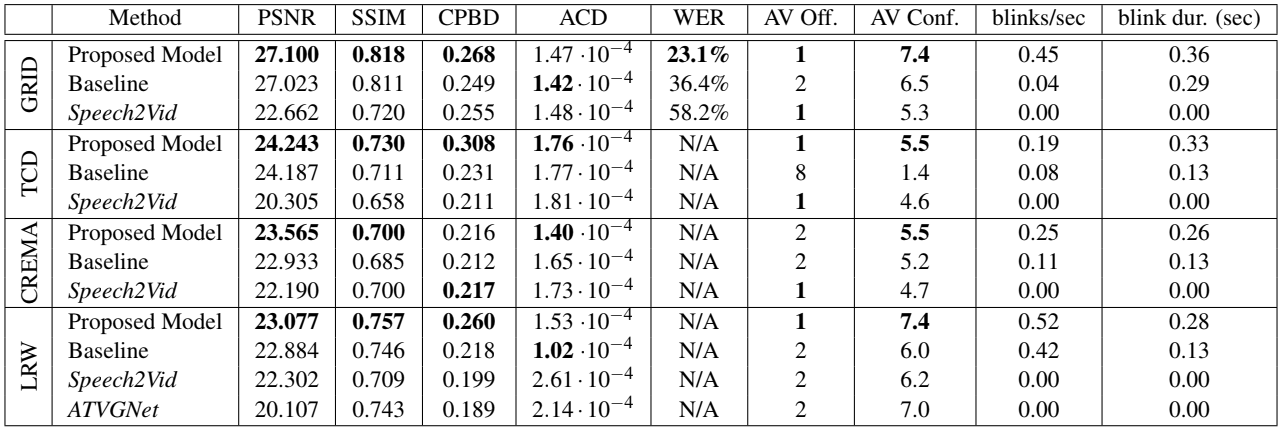
\includegraphics[width=15cm]{./content/images/vou2020_result.png}
    \caption{Kết quả đo đạc của tác giả}
    \label{fig:vou2020_result}
\end{figure}

Qua bảng này, ta thấy độ đo WER là rất thấp so với các mô hình khác nhờ vào sự phù hợp của vùng miệng so với ngữ điệu và nội dung tiếng nói. Các độ đo cơ bản khác như PSNR, SSIM và CPBD cũng được cải thiện so với các mô hình khác. Độ lệch về hình ảnh - âm thanh (AV Off.) cũng rất nhỏ (1). Điểm tự tin về sự đồng bộ giữa hình ảnh - âm thanh (AV Confident) được cải thiện rõ rệt và là bước tiến lớn so với các mô hình khác. Chuyển động của mắt cũng được đo đạc về số lần nháy mắt mỗi giây và thời lượng của một cái nháy mắt. Chuyển động của mắt trong video cũng là rất tự nhiên và đúng với chuyển động nháy mắt của người về tần số và thời lượng.
Ngoài các ưu điểm kể trên, một số yếu điểm từ nghiên cứu cũ được nêu ở phần \ref{sec:vougioukas2019} vẫn chưa được giải quyết. Đó là các yếu điểm về mặt biểu cảm trên gương mặt và chưa thể hiện được chuyển động của đầu. Ngoài ra, nghiên cứu cũng chưa chú trọng việc tái hiện lại môi trường xung quanh trong video. Qua kiểm nghiệm thực tế, mô hình còn cho thấy một yếu điểm khác khi không giữ được đặc điểm gương mặt của người mẫu nếu hình ảnh người này không tồn tại trong tập dữ liệu huấn luyện. Tác giả đã chạy thử mô hình với hình ảnh người châu Á (mô hình được huấn luyện với bộ dữ liệu mặt người phương Tây), mô hình cho ra mặt người đang nói với đặc trưng gương mặt không còn giống với người châu Á và không giữ được các đường nét đặc trưng của gương mặt người mẫu.

%------------------------------------------------------------------------

\section{Bài nghiên cứu "Hierarchical Cross-Modal Talking Face Generation with Dynamic Pixel-Wise Loss"\cite{chen2019}}

Nghiên cứu của Lele Chen vào năm 2019 có cùng mục tiêu với các nghiên cứu của Vougioukas, đó là tạo sinh chuỗi hình ảnh mặt người phù hợp với tiếng nói với đầu vào là một ảnh tĩnh của người mẫu và một đoạn âm thanh chứa tiếng nói. Trong nghiên cứu này, Chen đã đề xuất phương pháp mạng GANs nối tiếp để thiết kế bộ tạo sinh và phân biệt ảnh nhằm mục đích loại bỏ các đặc trưng không liên quan nhau trong miền đặc trưng ẩn. Nghiên cứu cũng làm rõ tầm quan trọng của việc sử dụng các đặc trưng trung gian thay vì sử dụng trực tiếp các đặc trưng được tổng hợp từ đầu vào. Nghiên cứu cũng sử dụng cơ chế chú ý (attenttion) để đánh dấu các điểm có sự biến đổi mạnh trên khuôn mặt dựa trên các đặc trưng ẩn được trích xuất. Cơ chế mạng phân biệt hồi quy cũng được tác giả giới thiệu nhằm mục đích giúp cho mạng phân biệt trích xuất đặc trưng có quan tâm đến thời gian để có thể dễ dàng phân biệt giữa video thật và video được tạo sinh. Qua đó, Lele Chen đã đóng góp thêm nhiều phương pháp mới để tạo sinh khuôn mặt và hạn chế sự giả tạo trong ảnh đầu ra. 

\begin{figure}[H]
    \centering
    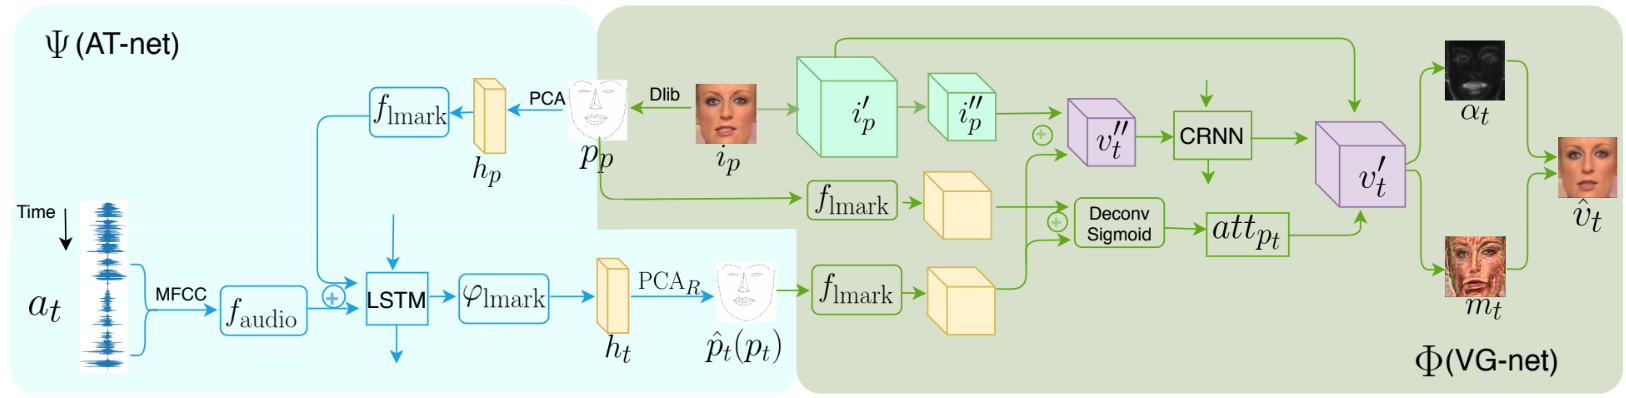
\includegraphics[width=15cm]{./content/images/chen2019_model.png}
    \caption{Mô hình được đề xuất bới nghiên cứu Hierarchical Cross-Modal Talking Face Generation with Dynamic Pixel-Wise Loss}
    \label{fig:chen2019_model}
\end{figure}

Hình \ref{fig:chen2019_model} thể hiện kiến trúc chung của mô hình được đề xuất. Mô hình tạo sinh ảnh được chia thành hai phần chính: phần trích xuất đặc trưng âm thanh $\Psi$ (AT-net) và phần tạo sinh hình ảnh $\Phi$ (VG-net). Với việc chia cấu trúc tổng quan thành hai phần nối tiếp nhau, ta có công thức thể hiện cơ chế tính toán của mạng:

\begin{subequations}
    \begin{equation}
        \hat{p}_{1:T} = \Psi(a_{1:T}, p_p)
    \end{equation}
    \begin{equation}
        \hat{v}_{1:T} = \Phi(\hat{p}_{1:T}, i_p, p_p)
    \end{equation}
\end{subequations}

Với $a_{1:T}$ là tín hiệu tiếng nói, $i_p$ là hình khuôn mặt của người mẫu, $p_p$ là các cột mốc (landmark) được trích xuất trên hình $i_p$, mô hình sẽ tạo sinh ra các cột mốc tương ứng với âm thanh $\hat{p}_{1:T}$ và dựa trên các cột mốc đó để dựng lại hình ảnh khuôn mặt $\hat{v}_{1:T}$.

Đầu tiên, các cột mốc trong ảnh mẫu $i_p$ được trích xuất bằng thư viện Dlib dùng phương pháp HOG. Bộ $\Psi$ (AT-net) nhận vào cột mốc $p_p$, sau đó dùng phương pháp PCA để thu giảm số chiều của vector cột mốc thành một vector đặc trưng $h_p$. Với việc sử dụng PCA, ngoài tác dụng giảm số chiều, tác giả còn có mục đích giảm nhiễu trên dữ liệu, từ đó giúp loại bỏ các chuyển động không mong muốn và các chuyển động không liên quan đến tiếng nói của các cột mốc như sự di chuyển của đầu, sự chuyển động của máy thu hình. Một bộ encoder $f_{lmark}$ được sử dụng để trích xuất đặc trưng cho các cột mốc. Đồng thời, tín hiệu âm thanh $a_{1:T}$ cũng được chuyển sang miền tần số  nhờ MFCC và được trích xuất đặc trưng nhờ bộ encoder $f_{audio}$. Vector đặc trưng cột mốc sẽ được ghép nối với tất cả vector đặc trưng tiếng nói theo kênh và đưa vào một bộ LSTM. Bộ LSTM hoạt động theo chiến thuật teacher forcing để sinh ra chuỗi các trạng thái ẩn (hidden state). Chuỗi trạng thái này được sử dụng như đặc trưng đầu ra và được đưa vào bộ decoder $\phi_{lmark}$ để tạo ra vector đặc trưng $h_t$ thể hiện các đặc trưng cột mốc của gương mặt sẽ được tạo sinh. Để tạo sinh ra cột mốc đó, ta dùng phép PCA ngược $PCA_R$ để đưa $h_t$ về chiều không gian của ma trận cột mốc và từ đó sinh ra cột mốc được dự đoán $\hat{p}_t$. Với việc sử dụng đặc trưng âm thanh và cột mốc để tạo sinh cột mốc mới theo thời gian thay vì trực tiếp sử dụng hình ảnh, nghiên cứu đã chỉ ra cách để tách biệt mục tiêu tái tạo chính xác khẩu hình miệng với các mục tiêu khác. Nhờ đó khẩu hình miệng được tái tạo chính xác hơn so với các nghiên cứu trước đó.

\begin{subequations}
    \begin{equation}
        v''_t = f_{img}(i_p) \oplus (f_{lmark}(\hat{p}_t) - f_{lmark}(p_p))
        \label{eqn:chen2019_vgnet_1}
    \end{equation}
    \begin{equation}
        att_{p_t} = \sigma(f_{lmark}(p_t) \oplus f_{lmark}(p_p))
        \label{eqn:chen2019_vgnet_2}
    \end{equation}
    \begin{equation}
        v'_t = (CRNN(v''_t)) \odot att_{p_t} + i'_p \oplus (1 - att_{p_t})
        \label{eqn:chen2019_vgnet_3}
    \end{equation}
\end{subequations}

Mạng tạo sinh ảnh $\Phi$ (VG-net) được xây dựng với mục tiêu duy trì các đặc tính trên khuôn mặt mẫu được cho ban đầu và tạo sự ổn định, liền lạc cho sự chuyển động giữa các khung hình. Hình ảnh mẫu $i_p$ được trích đặc trưng bằng một Convolution encoder và tạo ra tensor $i''_p$. Đồng thời, cột mốc $p_p$ và $\hat(p)_t$ cũng được trích đặc trưng nhờ các bộ encoder $f_{lmark}$. Tác giả giả định rằng sự sai lệch giữa vector cột mốc được tạo sinh $\hat{p_t}$ và cột mốc trong ảnh mẫu $p_p$ sẽ tương ứng với sự sai lệch trong hình ảnh mặt người được tạo sinh và ảnh mẫu. Vì vậy, đặc trưng sai khác này được kết hợp với đặc trưng ảnh mẫu bằng cách nối tiếp theo kênh để tạo ra đặc trưng ảnh mới (công thức \ref{eqn:chen2019_vgnet_1}). Cũng với việc kết hợp đặc trưng cột mốc ảnh mẫu và cột mốc ảnh được tạo sinh, ta sẽ tìm được các vùng trên gương mặt có sự thay đổi lớn bằng các chuyển động của các cột mốc tương ứng nhau. Từ đó, ta có thể tính được ma trận chú ý (attention map) để đánh dấu các vùng có sự thay đổi lớn trên ảnh (công thức \ref{eqn:chen2019_vgnet_2}). Khối CRNN là một khối đạng encoder - decoder, chứa trong nó là các khối Convolution - RNN, các khối Residual và các lớp Deconvolution. Đặc trưng $v''_t$ theo thời gian được đưa qua khối CRNN để encode và decode nó trở lại, kết hợp với $att_{p_t}$ và $i'_p$ để tạo thành tensor đặc trưng $v't$ (công thức \ref{eqn:chen2019_vgnet_3}). Việc đưa $v''_t$ qua CRNN là để liên kết các chuyển động theo thời gian và tạo sinh đặc trưng có tính liên kết về mặt thời gian. Do mức độ ảnh hưởng của tiếng nói đối với các cột mốc trên ảnh là khác nhau, ma trận $att_{p_t}$ được nhân vào đặc trưng ngõ ra của CRNN để chọn lấy các cột mốc bị ảnh hưởng nhiều bởi tiếng nói, các cột mốc còn lại được lấy từ đặc trưng ảnh mẫu $i'_p$. Sau cùng, đặc trưng tổng hợp $v'_t$ sẽ được dùng để sinh ra một ma trận chú ý $\alpha_t$ và ảnh mô tả chuyển động $m_t$. $\alpha_t$ được sinh ra nhờ việc cho $v'_t$ đi qua một lớp Convolution và hàm kích hoạt Sigmoid, trong khi $m_t$ được sinh ra nhờ cho $v'_t$ đi qua một lớp Convolution khác với hàm kích hoạt $tanh$. Trong khi $\alpha_t$ có khả năng đánh dấu các điểm ảnh có nhiều sự thay đổi trên ảnh được tạo sinh so với ảnh gốc bằng các giá trị xác suất cao, $m_t$ là một ảnh miêu tả chuyển động trên gương mặt tương ứng với âm thanh tại thời điểm $t$. Để có kết quả tạo sinh hoàn hảo, ổn định và giống với người mẫu nhất, ta sẽ kết hợp ảnh $m_t$ với ảnh $i_p$ ban đầu với tỉ lệ nhìn thấy của mỗi điểm ảnh trên mỗi ảnh được thể hiện qua ma trận chú ý $\alpha_t$. Ảnh đầu ra cuối cùng $\hat{v}_t$ được tạo sinh như sau: 

\begin{equation}
    \hat{v}_t = \alpha_t \odot m_t + (1 - \alpha_t) \odot i_p
\end{equation}

\begin{equation}
    \mathcal{L}_{pix} = \sum^{T}_{t=1} \Vert (v_t - \hat{v}_t) \odot (\overline{\alpha}_t + \beta) \Vert_1
    \label{eqn:chen2019_pix_loss}
\end{equation}

Hàm mất mát theo điểm ảnh được sử dụng trong công thức (\ref{eqn:chen2019_pix_loss}) cho thấy nó chỉ quan tâm nhiều tới các điểm ảnh có trọng số cao trong ma trận $\alpha_t$. $\beta$ là một hằng số, được cộng thêm vào hàm mất mát nhằm mục đích đảm bảo điểm ảnh nào cũng có đóng góp vào hàm mất mát, tránh hiện tượng $\alpha_t$ về 0.

\begin{figure}[H]
    \centering
    \begin{minipage}{0.48\textwidth}
        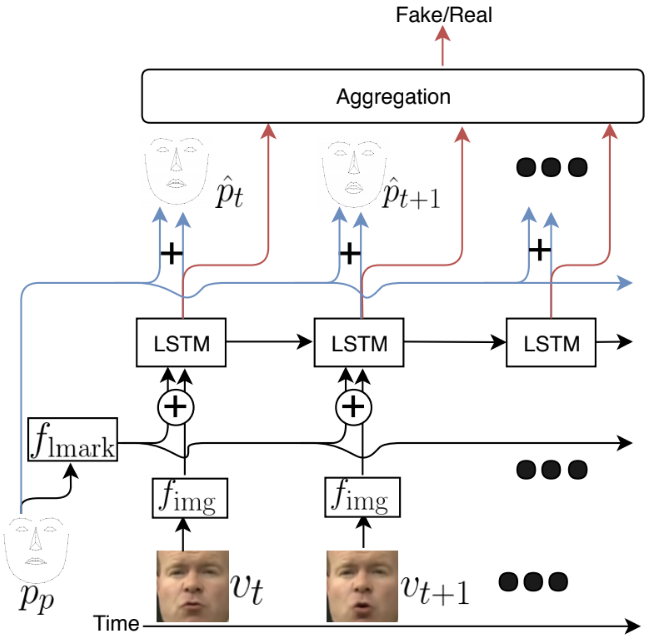
\includegraphics[width=7cm]{./content/images/chen2019_dis.png}
        \caption{Kiến trúc bộ phân biệt}
        \label{fig:chen2019_dis}
    \end{minipage}\hfill
    \begin{minipage}{0.48\textwidth}
        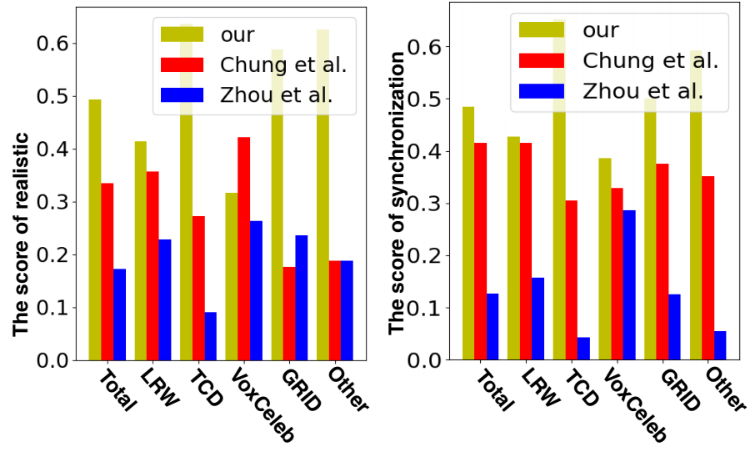
\includegraphics[width=7cm]{./content/images/chen2019_score.png}
        \caption{So sánh kết quả các mô hình}
        \label{fig:chen2019_score}
    \end{minipage}
\end{figure}

Bộ phân biệt được thiết kế để phân biệt chuỗi hình ảnh được đưa vào $v_t$ là chuỗi hình ảnh thật từ video hay chuỗi hình ảnh được tạo sinh. Bộ phân biệt này có chức năng phân biệt tổng quát trên toàn bộ chuỗi ảnh và cho từng ảnh một trong chuỗi. Công thức của bộ phân biệt được thể hiện như sau:

\begin{subequations}
    \begin{equation}
        \begin{split}
            \hat{p}_t &= D_p(p_p, v_t) \\
            &= p_p + LSTM(f_{lmark}(p_p) \oplus f_{img}(v_t))
        \end{split}
        \label{eqn:chen2019_dis_dp}
    \end{equation}
    \begin{equation}
        \begin{split}
            s &= D_s(p_p, v_{1:T}) \\
            &= \sigma(\frac{1}{T} \sum^T_{t=1} LSTM(f_{lmark}(p_p) \oplus f_{img}(v_t)))
        \end{split}
        \label{eqn:chen2019_dis_ds}
    \end{equation}
    \begin{equation}
        \begin{split}
        \mathcal{L}_{gan} = &\mathbb{E}_{p_p,v_{1:T}}[logD_s(p_p,v_{1:T})]+\\
        &\mathbb{E}_{p_p,v_{1:T},i_p}[log(1-D_s(p_p,G(p_p,p_{1:T},i_p)))]+\\
        &||(D_p(p_p,G(p_p,p_{1:T},i_p))-p_{1:T}) \odot M_p||^2_2+\\
        &||(D_p(p_p,v_{1:T})-p_{1:T}) \odot M_p||^2_2
        \end{split}
        \label{eqn:chen2019_dis_gan}
    \end{equation}
\end{subequations}

Kết quả đo đạc của tác giả được thể hiện ở bảng sau:
\begin{figure}[H]
    \centering
    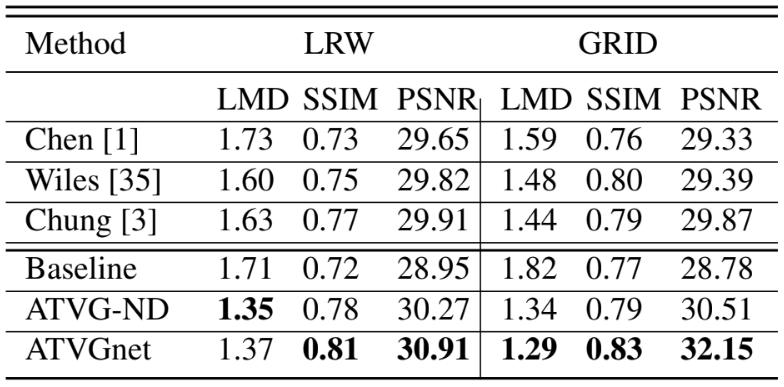
\includegraphics[width=10cm]{./content/images/chen2019_result.png}
    \caption{}
    \label{fig:chen2019_result}
\end{figure}

Qua bảng này, ta thấy nghiên cứu của tác giả đã có sự cải tiến khi làm giàu thêm tri thức của mạng về bài toán với việc thay thế đặc trưng âm thanh bằng các cột mốc gương mặt. Và với bộ phân biệt, không chỉ học được cách nhận biết ảnh thật và giả như các nghiên cứu trước mà còn học được cách tạo dựng lại các cột mốc trên gương mặt ban đầu. Nhờ đó mạng phân biệt có nhiều tri thức hơn để giúp điều chỉnh mạng tạo sinh nhằm tạo ra những chuyển động chân thật cho gương mặt. Thiết kế của mạng không nhằm mục đích tạo sinh hoàn toàn hình ảnh khuôn mặt, mà thay vào đó, mạng chỉ cố gắng mô tả những thay đổi phải thực hiện trên hình ảnh mẫu để tạo ra ảnh tạo sinh. Điều này làm cho hình ảnh tạo sinh có chất lượng tốt và giữ được đặc trưng riêng của người mẫu.

% \chapter{Phương pháp đề xuất}
% Trình bày chi tiết về ý tưởng, các mô hình toán, các chứng minh nếu có. Đồng thời trình bày các bước thực hiện và khảo sát, kiểm nghiệm kết quả nghiên cứu. Mô tả kết quả nghiên cứu khi thử nghiệm với nhiều tập dữ liệu và những độ khó khác nhau.

\section{Ý tưởng thực hiện luận văn}

Nhắc lại yêu cầu bài toán: Tạo sinh video khuôn mặt người đang nói dựa trên một hình ảnh tĩnh chứa mặt người mẫu và một đoạn âm thanh chứa tiếng nói. Qua yêu cầu bài toán ta thấy, đầu vào của hệ thống có tính chất khác với đầu ra, sử dụng hình ảnh tĩnh và âm thanh để tạo ra hình ảnh chuyển động. Một số yêu cầu quan trọng khác quyết định chất lượng của chuỗi hình ảnh được tạo sinh ra cũng cần được chú ý. Đó là:
\begin{itemize}
    \item Hình ảnh phải chân thật, rõ ràng, thể hiện được đúng hình dáng gương mặt người đang nói, không bị méo mó, dị dạng.
    \item Chuỗi hình ảnh được tạo sinh cần phải giữ được đặc trưng gương mặt trong ảnh mẫu. Có nghĩa là, người xem vẫn có thể nhận ra được mặt người đang nói trong video được tạo sinh chính là người trong hình ảnh ban đầu
    \item Khẩu hình miệng khi chuyển động phải khớp với âm thanh được nói ra. Sự chuyển động của môi và miệng trong video được tạo sinh phải thể hiện được cách phát âm từ được nói gần như trong thực tế
\end{itemize}

Dựa theo yêu cầu bài toán, ta cần tìm kiếm một phương pháp để kết hợp đặc trưng âm thanh và hình ảnh lại với nhau, sau đó chuyển đổi đặc trưng này thành video. Để mang lại sự trung thực, sắc nét cho hình ảnh được tạo sinh cũng như lưu giữ được các đặc trưng khuôn mặt người trong hình ảnh ban đầu, chiến thuật của ta là sẽ dựa hoàn toàn trên hình ảnh ban đầu để tạo sinh các khung hình khác trong video. Như vậy, với mỗi khung hình ở mỗi thời điểm $t$ trên video, ta cần phải tìm kiếm sự thay đổi của khung ảnh tại thời điểm đó so với hình ảnh tĩnh được cho ban đầu. Sau đó, ta thực hiện biến đổi hình ảnh được cho ban đầu thành hình ảnh ở khung hình tại thời điểm $t$. Như vậy, câu hỏi đặt ra là ta cần phải thay đổi tại vùng nào trên ảnh mẫu và tại những vùng đó ta sẽ thay đổi như thế nào, thay đổi nhiều hay ít.

Sự thay đổi của hình ảnh được quyết định phần nhiều bởi chuỗi âm thanh được đưa vào hệ thống. Âm thanh giọng nói quyết định khẩu hình miệng và các biểu cảm trên gương mặt, đôi khi còn có thể quyết định cách chuyển động của đầu. Tuy giọng nói góp phần lớn khi định hình sự thay đổi trên gương mặt, ảnh mẫu ban đầu cũng quyết định phần nào các thay đổi đó. Hình ảnh ban đầu cung cấp thông tin về nhận dạng khuôn mặt, về những đặc điểm của các bộ phận trên gương mặt người nói, về vị trí của mắt, mũi, miệng để định hình cách âm thanh thay đổi hình dạng gương mặt.

\begin{figure}[H]
    \centering
    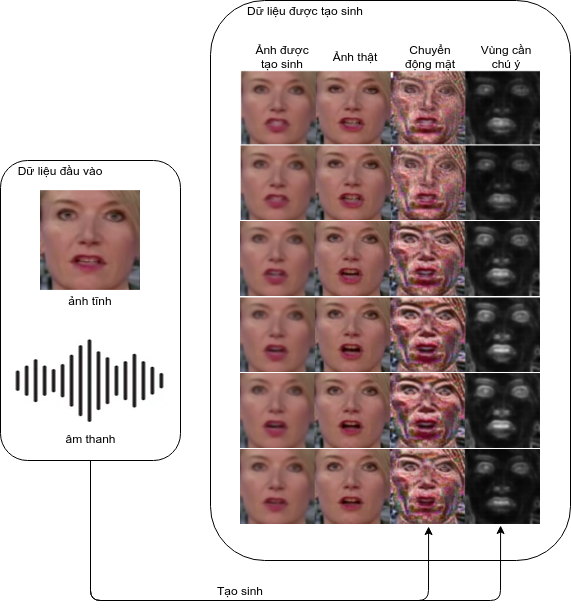
\includegraphics[width=12cm]{./content/materials/idea.png}
    \caption{Ý tưởng về tạo sinh chuỗi hình ảnh chuyển động cho mặt người đang nói}
\end{figure}

Ý tưởng giải quyết bài toán được thể hiện ở hình trên. Chúng ta sẽ tạo ra một hệ thống có khả năng trích xuất đặc trưng của hình ảnh tĩnh ban đầu và âm thanh giọng nói để tạo ra hình ảnh chuyển động của mặt. Tuy nhiên, hình ảnh chuyển động mặt này không hoàn toàn được sử dụng, mà song song với nó, ta tạo ra một mặt nạ tương ứng. Mặt nạ này chỉ chú ý tới một số khu vực trên hình ảnh chuyển động mặt được tạo sinh. Những vùng màu đen là những vùng không được chú ý đến trên ảnh chuyển động vừa được sinh ra, ngược lại, các vùng có màu trắng càng sáng thì càng được chú ý. Như vậy, mặt nạ chú ý sẽ cho ta biết ta nên thay đổi những vùng nào trên gương mặt tại thời điểm $t$ tương ứng với tiếng nói ở thời điểm đó. Đồng thời, hình ảnh chuyển động mặt được tạo sinh song song cho ta biết ta phải thay đổi như thế nào ở những điểm được chú ý. Ở những điểm không được chú ý còn lại, ta sẽ thay thế bằng các điểm ảnh trong ảnh gốc ban đầu. Nhờ vậy, ta có thể bảo toàn được nhận dạng của người nói trong quá trình tạo sinh bằng việc chỉ tìm ra những điểm thay đổi trên gương mặt thay vì cố gắng tìm cách tạo sinh toàn bộ gương mặt của người nói.

\section{Mô hình hóa bài toán}\label{sec:modeling}

Như phân tích ở phần trên, âm thanh sẽ đóng góp phần lớn vào việc tạo sinh chuyển động cho khuôn mặt. Tuy nhiên, ta thấy dữ liệu dạng sóng biên độ - thời gian của âm thanh dường như không có mối liên hệ tốt với chuyển động trên gương mặt. Vì thế, ta cần xử lý âm thanh để tạo ra một đặc trưng gần gũi hơn với những chuyển động tương ứng trên gương mặt. Đây là một bước cần thiết để hình ảnh được tạo sinh có chất lượng tốt và có được những chuyển động chính xác. Do đó, ta sẽ chuyển âm thanh thành một dạng thể hiện khác, đó là các cột mốc trên gương mặt (Facial Landmark). Cột mốc trên mặt gồm 68 điểm trên không gian hai chiều, mỗi điểm đánh dấu một vị trí trên gương mặt, hình sau cho là ví dụ về cột mốc trên gương mặt người:

\begin{figure}[H]
    \centering
    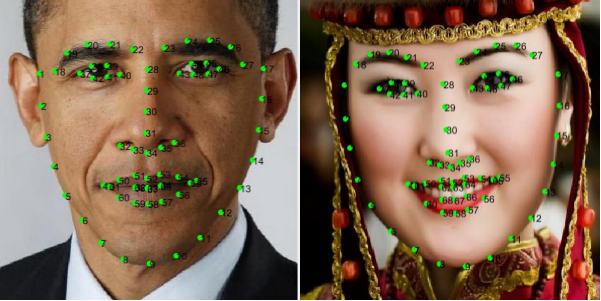
\includegraphics[width=10cm]{./content/materials/landmark_intro.png}
    \caption{Các điểm cột mốc trên khuôn mặt. Hình ảnh được lấy từ bài báo \cite{landmark}}
\end{figure}

Như vậy, từ đoạn âm thanh có chứa tiếng nói và hình ảnh ban đầu, ta sẽ tạo sinh ra một chuỗi cột mốc khuôn mặt để thay thế cho âm thanh làm căn cứ cho những chuyển động trên gương mặt. Cấu trúc tổng quát của hệ thống được thể hiện ở Hình \ref{fig:common_architecture}.

\begin{figure}[H]
    \centering
    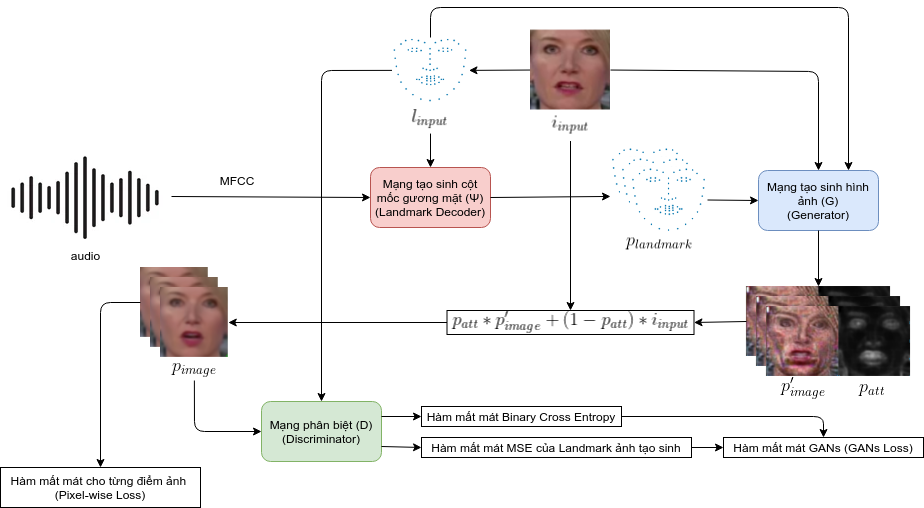
\includegraphics[width=15cm]{./content/materials/common_architecture.png}
    \caption{Cấu trúc tổng quát của hệ thống}
    \label{fig:common_architecture}
\end{figure}

Theo như kiến trúc được thể hiện ở Hình \ref{fig:common_architecture}, hệ thống sẽ trích xuất đặc trưng cột mốc $l_{input}$ trên gương mặt trong hình mẫu $i_{input}$. Sau đó, đặc trưng MFCC sẽ được trích xuất từ âm thanh đầu vào. Đặc trưng MFCC và $l_{input}$ sẽ được đưa vào mạng tạo sinh cột mốc gương mặt (Landmark Decoder). Mạng này kết hợp hai đặc trưng trên với nhau để dự đoán chuỗi các cột mốc gương mặt người khi nói đoạn âm thanh được đưa vào hệ thống ($p_{landmark}$). Từ thời điểm này, âm thanh không còn được sử dụng để tạo sinh hình ảnh mặt người, chuỗi những điểm cột mốc gương mặt $p_{landmark}$ sẽ thay thế cho âm thanh trong những bước xử lý tiếp theo. Như vậy, ta đã tách rời được dữ liệu âm thanh so với phần tạo sinh hình ảnh, và cung cấp cho phần mạng phía sau những đặc trưng dễ học hơn, giàu thông tin hữu ích hơn và ít nhiễu hơn. 

Phần tiếp theo trong hệ thống là cặp mạng tạo sinh (Generator) và phân biệt (Discriminator) tạo nên mạng GANs như đã trình bày ở phần \ref{sec:base_knowledge_gans}. Tuy nhiên, đây không phải là mạng GANs truyền thống mà là mạng GANs có điều kiện (Conditional GANs \cite{conditional_gan}). Thay vì tạo sinh dữ liệu bằng một véc tơ được sinh ra ngẫu nhiên theo phân phối chuẩn, mạng GANs có điều kiện dựa vào một điều kiện đầu để tạo sinh dữ liệu. Trong luận văn này, mạng GANs có điều kiện tạo sinh dữ liệu với điều kiện đầu vào là $i_{input}$, $l_{input}$ và $p_{landmark}$ được cho trước.

Bài toán mà mạng tạo sinh phải giải là đối với mỗi khung ảnh được tạo sinh để phù hợp với giọng nói được cho, ta phải thay đổi hình ảnh gốc $i_{input}$ ở những vị trí nào, và tại vị trí đó, ta phải thay đổi nó như thế nào để sinh ra được hình ảnh mới? Mạng tạo sinh hình ảnh với đầu vào là hình ảnh mẫu $i_{input}$, cột mốc của gương mặt trên hình ảnh mẫu $l_{input}$ và chuỗi cột mốc gương mặt vừa được tạo sinh $p_{landmark}$ có chức năng tạo sinh ra hai chuỗi dữ liệu $p_{att}$ và $p'_{image}$ tương ứng để trả lời cho câu hỏi trên. Chuỗi hình ảnh $p_{att}$ và $p'_{image}$ có cùng chiều dài và kích thước hình ảnh. Chuỗi hình ảnh $p_{att}$ thể hiện những điểm cần thay đổi trên ảnh gốc và mức độ thay đổi tại điểm đó. Chuỗi dữ liệu còn lại là chuỗi $p'_{image}$ thể hiện những thay đổi trên ảnh gốc để phù hợp với tiếng nói trong âm thanh. Chuỗi $p'_{image}$ có cấu trúc hình ảnh là gương mặt người, có sự thay đổi theo trục thời gian tương ứng với những chuyển động trên gương mặt để phù hợp với giọng nói. Tuy nhiên đây không phải là hình ảnh hoàn chỉnh của gương mặt, chỉ một vài chi tiết cần thiết trên chuỗi $p'_{image}$ được lấy ra và ghép vào ảnh gốc $i_{input}$ để tạo ra hình ảnh cuối cùng. Cũng vì vậy, $p'_{image}$ là chuỗi hình ảnh được sinh ra để cho ta biết hình ảnh gốc nên thay đổi như thế nào. 

Cuối cùng, ta cần phải kết hợp hình ảnh ban đầu $i_{image}$ và chuỗi hình ảnh vừa được sinh ra là $p'_{image}$ và $p_{att}$ lại để tạo thành chuỗi hình ảnh hoàn chỉnh $p_{image}$. Có thể gọi $p_{att}$ là một mặt nạ chú ý (attention mask), mặt nạ này có giá trị các điểm ảnh trong khoảng từ 0 đến 1. Với điểm ảnh càng gần về 0, điểm ảnh cùng vị trí trong $i_{input}$ càng được sử dụng nhiều, điểm ảnh cùng vị trí trong $p'_{image}$ càng ít được sử dụng và ngược lại. Công thức tạo thành $p_{image}$ được biểu diễn như sau:

\begin{equation}
    p_{image}=p_{att}*p'_{image}+(1-p_{att})*i_{input}
\end{equation}

Hình ảnh hoàn chỉnh được tạo sinh $p_{image}$ sau đó được đem đi so sánh với chuỗi hình ảnh trong video gốc để tính giá trị mất mát L1. Giá trị mất mát này được lan truyền ngược để cập nhật các trọng số trong mạng tạo sinh. Chuỗi hình ảnh hoàn chỉnh cũng được đưa vào bộ phân biệt (Discriminator) để bộ phân biệt dự đoán xem chuỗi hình ảnh này là ảnh được tạo sinh (chuỗi hình ảnh giả) hay chuỗi hình ảnh này là hình ảnh được lấy từ tập dữ liệu thật, sai sót của bộ phân biệt được biểu diễn bằng hàm Binary Cross Entropy. Đồng thời bộ phân biệt cũng dựa vào chuỗi hình ảnh được đưa vào và cột mốc gương mặt của ảnh mẫu $l_{input}$ để cố gắng sinh ra một chuỗi cột mốc gương mặt tương ứng với chuỗi hình ảnh $p_{image}$ được đưa vào mạng. Chuỗi cột mốc gương mặt vừa được sinh ra này sẽ được so sánh với chuỗi cột mốc gương mặt được rút trích trực tiếp từ chuỗi hình ảnh trong video gốc. Sự sai khác trong hai chuỗi cột mốc gương mặt được tính bằng hàm mất mát Mean Square Error. Điều này có nghĩa, chuỗi hình ảnh được tạo sinh $p_{image}$ phải rút trích được một chuỗi cột mốc gương mặt sao cho giống nhất với chuỗi cột mốc gương mặt trong video gốc. Tổng hợp của giá trị mất mát Mean Square Error và Binary Cross Entropy vừa nêu, ta được hàm mất mát GANs chung của mạng GANs. Giá trị mất mát GANs này được lan truyền ngược để cập nhật trọng số cho cả mạng tạo sinh và mạng phân biệt.

Tóm lại, việc tạo sinh hình ảnh từ đoạn âm thanh $a(t)$, hình ảnh mẫu $i_{input}$ và cột mốc gương mặt $l_{input}$ được biểu diễn dưới dạng công thức toán như sau:

\begin{equation}
    \begin{split}
    p_{landmark}(t) &= \Psi(l_{input}, mfcc(a(t)))\\
    p'_{image}(t), p_{att} &= G(i_{input}, l_{input}, p_{landmark})\\
    p_{image} &= p_{att}*p'_{image}+(1-p_{att})*i_{input}
    \end{split}
\end{equation}

\section{Tiền xử lý dữ liệu}

\subsection{Tiền xử lý âm thanh}
Ta có thể thấy, phần âm thanh ta chú ý đến chỉ là tiếng nói của con người và ta mong muốn loại bỏ các tạp âm khác. Khoảng tần số âm thanh mà con người có thể nghe được dao động trong khoảng từ 20Hz đến 20kHz, và theo như phương pháp lấy mẫu Nyquist, để lấy mẫu một tín hiệu có tần số $x$(Hz), thì bộ lấy mẫu phải lấy mẫu ở tần số ít nhất là $2x$(Hz). Như vậy, khi thu âm, để thu được âm thanh mà con người có thể nghe được, người ta phải lấy mẫu ở tần số thấp nhất là 40kHz. Trên thực tế, trong việc ghi âm, người ta thường lấy mẫu ở tần số 44.1kHz. Hình sau miêu tả các bước xử lý âm thanh trong bài nghiên cứu.

\begin{figure}[H]
    \centering
    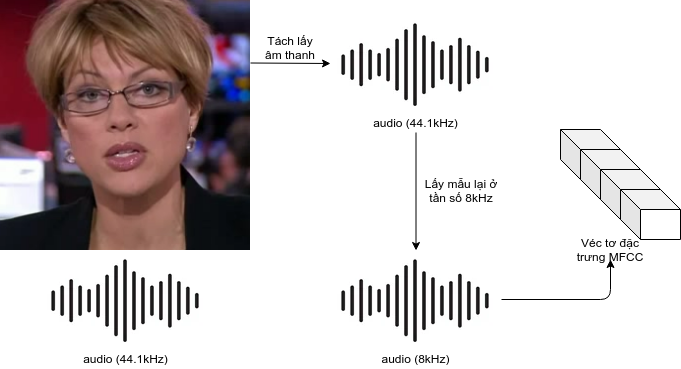
\includegraphics[width=12cm]{./content/materials/preprocess-audio.png}
    \caption{Tiền xử lý tín hiệu âm thanh}
\end{figure}

Tuy nhiên, thanh quản con người chỉ có thể phát ra âm thanh với tần số dưới 4kHz. Vì vậy, để loại bỏ nhiễu ở các dải tần số cao hơn, ta có thể lấy mẫu lại âm thanh trong video. Theo phương pháp lấy mẫu Nyquist, để lấy được âm thanh có tần số dưới 4kHz, ta cần phải lấy mẫu ở tần số 8kHz. Như vậy, tất cả âm thanh trong tất cả các đoạn video sẽ được lấy mẫu lại ở tần số 8kHz. Bộ lấy mẫu sẽ hoạt động như một bộ lọc thông thấp để loại bỏ nhiễu cao tần trong các đoạn âm thanh. Phương pháp lấy mẫu tần số thấp này cũng được dùng trong các thiết bị thu tiếng nói như máy thu âm, điện thoại để loại bỏ nhiễu.

Âm thanh sau khi lấy mẫu sẽ được đem đi trích xuất để lấy đặc trưng MFCC. Như đã nói ở phần \ref{sec:base_knowledge_mfcc}, MFCC là đặc trưng âm thanh chỉ dành riêng cho tiếng nói của con người. Ta tiến hành lấy đặc trưng MFCC với của sổ trượt 10ms, cứ mỗi cửa sổ trượt 10ms sẽ sinh ra một véc tơ 13 chiều tương ứng với 13 quãng tần số khác nhau, tuy nhiên ta sẽ loại bỏ khoảng tần số đầu do nó có tần số quá thấp và chỉ sử dụng 12 khoảng tần số ở cuối. Như vậy, mỗi cửa sổ 10ms theo trúc thời gian của âm thanh sẽ tạo ra một véc tơ 12 chiều, một đoạn âm thanh sẽ tạo thành một chuỗi véc tơ có chiều dài tương ứng với thời gian của nó.

\subsection{Tiền xử lý hình ảnh và trích xuất cột mốc gương mặt}\label{sec:preprocess_audio_lm}

Đầu tiên, tất cả các khung hình của tất cả các video sẽ được nhận diện khuôn mặt bằng mô hình nhận diện khuôn mặt của thư viện Dlib. Từ khung hình đã được nhận diện khuôn mặt này, ta dễ dàng tìm được cột mốc gương mặt trên từng khung hình. Với mỗi cột mốc gương mặt thu được, ta sẽ chuẩn hóa vùng mắt của nó sao cho 2 điểm ngoài của mắt (điểm 37 và 46 trên hình \ref{fig:standard_landmark}(a)) về tọa độ $(0.3, 0.33)$ và $(0.7, 0.33)$ tương ứng. Việc chuẩn hóa này được thực hiện nhờ phép biến đổi tương tự(Similarity Transformation) trên không gian hai chiều, nhờ đó mà tỉ lệ gương mặt gốc không bị thay đổi.

Cột mốc gương mặt chuẩn là cột mốc gương mặt có hình dáng chung chung của mặt người, và không có chứa đặc điểm riêng của gương mặt của bất kì người nào. Như vậy, để tìm ra cột mốc gương mặt chuẩn, ta cần tính giá trị trung bình của một số lượng lớn các cột mốc gương mặt trong các tập dữ liệu hiện có. Cột mốc gương mặt dùng làm chuẩn $l_{standard}$ được tính toán bằng cách lấy trung bình cộng của tất cả những cột mốc gương mặt đã được chuẩn hóa phần mắt như đã miêu tả ở trên.

\begin{figure}[H]
    \centering
    \subfloat[Cột mốc gương mặt đánh số]{{\includegraphics[width=7cm]{./content/materials/enum_landmark.png} }}
    \qquad
    \subfloat[Cột mốc gương mặt được dùng làm chuẩn $l_{standard}$]{{\includegraphics[width=7cm]{./content/materials/standard_landmark.png} }}
    \caption{Xử lý cột mốc gương mặt}
    \label{fig:standard_landmark}
\end{figure}

Tuy nhiên, video đôi khi được quay từ rất nhiều góc độ khác nhau của khuôn mặt, nên việc chuẩn hóa trở nên khó khăn hơn. Vì vậy, ngoài bước xử lý dời điểm 37 và 46, ta cần thêm một số bước xử lý sau để chuẩn hóa cột mốc gương mặt:
\begin{enumerate}
    \item Tính toán cột mốc gương mặt trung bình $l_{avg}$ của tất cả các cột mốc trong video
    \item Để giữ được tỉ lệ của khuôn mặt gốc, ta tính toán một phép biến đổi tương tự (Similarity Transformation) $t_{landmark}$ để chuyển những điểm cột mốc từ số 28 đến số 48 trên cột mốc trung bình $l_{avg}$ thành các điểm tương ứng trên cột mốc chuẩn $l_{standard}$
    \item Áp dụng phép biến đổi $t_{landmark}$ cho từng cột mốc gương mặt riêng lẻ trong video để tạo ra chuỗi cột mốc gương mặt mới đã được điều chỉnh $l_{mod}$
    \item Tìm trong $l_{mod}$ một cột mốc gương mặt có độ mở miệng (khoảng cách giữa điểm 63 và điểm 67) gần với cột mốc gương mặt chuẩn nhất, gọi cột mốc gương mặt đó là $l_{pivot}$
    \item Tìm độ sai lệch $l_{mod-diff}$ của tất cả các cột mốc gương mặt trong $l_{mod}$ so với cột mốc $l_{pivot}$: $l_{mod-diff} = l_{mod} - l_{pivot}$, sau đó tính tổng tích lũy $l_{cumsum}$ của $l_{mod-diff}$. Ta sử dụng cách này như một phương pháp để tách lấy chuyển động tương đối của cột mốc gương mặt ở thời điểm $t$ so với $l_{pivot}$ và bỏ đi các chi tiết đặc trưng của từng gương mặt khác nhau. Tiếp theo, ta cần phải chuyển tất cả các chuyển động này lên $l_{standard}$.
    \item Tìm một phép biến đổi Affine $t_{pivot}$ để chuyển $l_{pivot}$ thành $l_{standard}$. Tuy nhiên ta sẽ không sử dụng trực tiếp ma trận này mà sẽ chỉ sử dụng các hệ số của nó để tính toán ra hệ số phóng đại $s_x$ và $s_y$ tương ứng với từng sự sai lệch ở trục $x$ và $y$ của cột mốc gương mặt trong $l_{cumsum}$ so với cột mốc gương mặt chuẩn $l_{standard}$. Hai số $s_x$ và $s_y$ được gộp lại vào ma trận $s$.
    \item Áp dụng hệ số phóng đại $s$ lên lên tất cả các cột mốc gương mặt trong $l_{cumsum}$, kết quả của phép chuyển đổi này cho biết sự sai lệch của cột mốc gương mặt chuẩn $l_{standard}$ so với cột mốc gương mặt được chuẩn hóa. Như vậy, để tìm ra cột mốc gương mặt được chuẩn hóa $l_{final}$, ta áp dụng công thức: $l_{final} = l_{standard} + l_{cumsum}*s$
    \item Cột mốc gương mặt sau khi xử lý vẫn còn bị ảnh hưởng bởi việc di chuyển đầu. Vì vậy, ta tiếp tục làm thêm một bước chuẩn hóa đơn giản để kéo phần mũi và miệng vào vị trí trung tâm trong khung hình. Theo đó, biến đổi Affine tiếp tục được sử dụng để dịch chuyển các điểm 28, 31, 34, 52, 58, 9 từ $l_{final}$ về các điểm tương ứng trên $l_{standard}$.
\end{enumerate}

Hình sau cho thấy hiệu quả của phép biến đổi trên. Cột mốc gương mặt gốc (màu xanh) bị biến dạng mạnh so với cột mốc chuẩn. Tuy nhiên qua phép biến đổi, ta đã phần nào khôi phục và xấp xỉ được hình dạng của cột mốc gương mặt nếu nhìn thẳng, đồng thời loại bỏ hoàn toàn đặc trưng khuôn mặt của cá nhân người nói. Cột mốc gương mặt này sẽ được dùng để huấn luyện mạng.

\begin{figure}[H]
    \centering
    \includegraphics[width=15cm]{./content/materials/standardize_landmark.png}
    \caption{Kết quả chuẩn hóa cột mốc gương mặt. Đỏ - sau chuẩn hóa, xanh - cột mốc gương mặt gốc}
\end{figure}

Sau khi có được cột mốc gương mặt được chuẩn hóa $l_{final}$, ta tiến hành chuẩn hóa hình ảnh khuôn mặt để chuẩn bị dữ liệu hình ảnh cho việc huấn luyện. Hình ảnh mặt người cần được cắt ra từ video gốc là một khung hình vuông, có kích thước 128x128 điểm ảnh quay trực tiếp vào mặt người đang nói. Khung hình phải đảm bảo chứa tất cả các thành phần của khuôn mặt. Khuôn mặt được chuẩn hóa dựa trên việc biến đổi của các thành phần trên cột mốc gương mặt ở bước chuẩn hóa trước. Qua đó, ta so sánh sự biến đổi từ cột mốc gương mặt sau khi được chuẩn hóa vùng mắt với cột mốc chuẩn $l_{standard}$. Trên mỗi video, đối với từng khung hình, ta lần lượt tìm biến đổi Affine để chuyển các điểm cột mốc 28, 31, 34, 49, 55 từ cột mốc gương mặt ban đầu thành cột mốc chuẩn $l_{standard}$. Ta sử dụng ma trận biến đổi này để áp dụng lên khung hình thô của video, nhằm tạo ra một góc nhìn khác nhau cho từng khung hình mà tại đó gương mặt ít bị biến đổi trong quá trình di chuyển và ăn khớp nhất với cột mốc chuẩn. Sau khi hình được biến đổi, ta sử dụng thư viện Dlib để cắt ảnh gương mặt từ trong khung hình này. Những khung hình này là những khung hình đã được chuẩn hóa và sẽ được đem đi huấn luyện mạng. Kết quả xử lý hình ảnh theo phương pháp trên được thể hiện ở hình sau.

\begin{figure}[H]
    \centering
    \includegraphics[width=15cm]{./content/materials/preprocess-image.png}
    \caption{Kết quả chuẩn hóa hình ảnh. Có 20 cặp hình, ở mỗi cặp hình thì hình bên phải là khung hình gốc, hình bên trái là gương mặt đã được cắt sau khi áp dụng phép biến đổi Affine}
\end{figure}


\section{Cấu trúc chi tiết của hệ thống}

Hệ thống tạo sinh hình ảnh được lấy ý tưởng từ bài báo \cite{chen2019} và được chia làm ba phần:
\begin{itemize}
    \item \textbf{Mạng giải mã cột mốc gương mặt (Landmark Decoder):} Mạng giải mã cột mốc gương mặt là một mạng nơ ron nhận đầu vào là đặc trưng MFCC của giọng nói và cột gốc gương mặt của khung hình mẫu. Như đã nói ở phần \ref{sec:modeling}, ta sẽ không sử dụng trực tiếp đặc trưng âm thanh ở phần mạng GANs vì nó không "gần" với đặc trưng hình ảnh. Vì vậy, mạng giải mã cột mốc gương mặt được dùng để tạo ra cột mốc gương mặt tương ứng với giọng nói trong âm thanh đã cho nhằm mục đích cung cấp một đặc trưng tốt hơn và gần hơn với hình ảnh gương mặt cần được tạo sinh.
    \item \textbf{Mạng tạo sinh hình ảnh (Generator):} Mạng tạo sinh hình ảnh với đầu vào là hình ảnh mẫu của người muốn tạo sinh, cột mốc gương mặt của ảnh và chuỗi cột mốc gương mặt được dự đoán bởi mạng giải mã cột mốc gương mặt. Đầu ra của mạng là chuỗi hình ảnh được tạo sinh hoàn chỉnh của gương mặt người đang nói. Mạng tạo sinh có chức năng trích xuất và tổng hợp các đặc trưng từ đầu vào, kết hợp chung với nhau theo trục không gian và thời gian để tạo ra hình ảnh chân thật và mượt mà nhất. Đây cũng là phần tạo sinh của mạng GANs được dùng trong bài
    \item \textbf{Mạng phân biệt hình ảnh (Discriminator):} Mạng phân biệt hình ảnh có đầu vào là chuỗi hình ảnh trong video gốc hoặc chuỗi hình ảnh được tạo sinh từ mạng tạo sinh, kèm theo đó là cột mốc gương mặt của hình mẫu. Đầu ra của mạng là điểm số xác suất dự đoán liệu chuỗi hình ảnh được đưa vào mạng có phải là chuỗi hình ảnh được trích xuất từ video thật hay chỉ là ảnh được tạo sinh bởi mạng tạo sinh. Ngoài ra mạng cũng cố gắng dự đoán cột mốc gương mặt trong chuỗi hình ảnh được đưa vào mạng nhằm mục đích tạo ra chuyển động khớp với video gốc hơn. Mạng phân biệt này kết hợp với mạng tạo sinh ở trên để tạo thành hệ thống mạng GANs.
\end{itemize}

\subsection{Cấu trúc của bộ giải mã cột mốc gương mặt (Landmark Decoder)}

Bộ giải mã cột mốc gương mặt là một mạng học sâu được ghép nối từ nhiều mạng nhỏ khác nhau, bao gồm mạng tích chập để rút trích đặc trưng MFCC (MFCC Encoder), mạng LSTM, và các mạng kết nối đầy đủ để chuyển các đặc trưng ở lớp cuối thành đầu ra cho mạng.

\begin{figure}[H]
    \centering
    \includegraphics[width=15cm]{./content/materials/landmark_decoder.png}
    \caption{Cấu trúc của bộ giải mã cột mốc gương mặt (Landmark Decoder)}
\end{figure}

Cấu trúc chi tiết của mạng được thể hiện ở hình trên. Như đã nói ở trên, âm thanh được trích xuất MFCC với cửa sổ 10ms, mỗi khung hình có thời lượng là 40ms (do video được thu ở tốc độ ghi hình 25FPS), do đó, tensor MFCC của 1 khung hình có kích thước 1x12x4. Tuy nhiên, để tạo ra được cột mốc gương mặt cho 1 khung hình, ta cần phải lấy đặc trưng MFCC của 3 khung hình trước nó, 3 khung hình sau nó và cả chính nó. Vậy, tổng cộng ta cần dùng đặc trưng âm thanh từ 7 khung hình. Như vậy, tensor MFCC để tạo sinh ra một khung hình có kích thước 1x12x28, vầ đây chính là kích thước của $mfcc(a_t)$. Mạng MFCC Encoder có chức năng trích xuất đặc trưng từ tensor $mfcc(a_t)$ bằng phương pháp tích chập. Mạng có 4 lớp tích chập, 4 lớp Batchnorm và 4 lớp kích hoạt ReLU để trích xuất các đặc trưng ban đầu. Các lớp kết nối đầy đủ ở cuối mạng được dùng để học các đặc trưng bậc cao và tạo ra véc tơ đầu ra có kích thước 256 chiều $v_{mfcc}(t)$. Với $N$ khung hình ở đầu vào, ta sẽ có được $N-6$ véc tơ tạo thành chuỗi véc tơ 256 chiều $v_{mfcc}$ do 3 khung hình đầu và 3 khung hình cuối không được sử dụng. Như vậy, tensor $v_{mfcc}$ có kích thước 256x(N-6)

Cột mốc trong ảnh mẫu sau khi được chuẩn hóa sẽ được thu gọn số chiều nhờ vào giải thuật PCA. Mục đích của việc sử dụng PCA ở đây là để loại bỏ các tác động từ chuyển động đầu của người nói. PCA Landmark Encoder là bộ trích xuất đặc trưng dùng các lớp kết nối đầy đủ nhằm trích xuất đặc trưng của đầu vào $v_{input}$ nhằm tạo ra véc tơ $v_{landmark-encoded}$ có chiều dài 512. Véc tơ $v_{landmark-encoded}$ được nối nối tiếp với từng véc tơ $v_{mfcc}(t)$ nhằm kết hợp đặc trưng cột mốc với đặc trưng âm thanh. Tại mỗi thời điểm $t$, đặc trưng này là một véc tơ có kích thước 768 chiều. Như vậy, sau khi kết hợp hai đặc trưng này lại bằng cách nối tiếp các véc tơ, ta sẽ có chuỗi véc tơ đặc trưng $v_{landmark-feature}$ có kích thước (N-6)x768. Mỗi véc tơ $v_{landmark-feature}(t)$ được đưa vào mạng LSTM theo thứ tự thời gian. Mạng LSTM là mạng có kích thước ẩn là 256. Vì vậy, với mỗi véc tơ $v_{landmark-feature}(t)$ được đưa vào mạng, ta sẽ có được một véc tơ đầu ra có chiều dài 256. Véc tơ đầu ra này được đưa vào mạng kết nối đầy đủ, với đầu ra là số chiều bằng với số chiều được dùng để lấy PCA cho $l_{input}$, với hàm kích hoạt là hàm Tanh để cho ra $v_{landmark-PCA}$. Với mỗi véc tơ $v_{landmark-PCA}(t)$, ta áp dụng phép lấy PCA ngược để tạo ra chuỗi cột mốc gương mặt $p_{landmark}$, và đây chính là chuỗi cột mốc gương mặt được dự đoán cho âm thanh ở đầu vào.

Tóm lại, mạng giải mã cột mốc được mô hình hóa bằng công thức toán như sau:

\begin{equation}
    \begin{split}
    v_{landmark-encoded} &= f_{landmark-encoder}(PCA(l_{input}))\\
    v_{mfcc}(t) &= f_{mfcc-encoder}(mfcc(a_t))\\
    v_{landmark-feature} &= LSTM(v_{landmark-encoded} \oplus v_{mfcc})\\
    p_{landmark} &= PCA_R(\varphi_{landmark}(v_{landmark-feature}))
    \end{split}
\end{equation}

Mạng giải mã cột mốc gương mặt (Landmark Decoder) được huấn luyện độc lập với các mạng còn lại do dữ liệu đã sẵn có ở đầu vào và đầu ra, cũng như để đơn giản hóa quá trình huấn luyện. Đầu ra của mạng là chuỗi các cột mốc gương mặt sẽ được dùng như đầu vào cho mạng GANs tạo sinh ảnh sẽ được nói đến trong phần tiếp theo. Mạng này được huấn luyện với hàm mất mát MSE truyền thống. Gọi $l_{original}$ là chuỗi cột mốc gương mặt được trích xuất từ đoạn video có chứa âm thanh được đưa vào đầu vào của mạng, hàm mất mát của mạng được biểu diễn như sau:

\begin{equation}
    \mathcal{L}_{landmark} = \frac{1}{n}\sum^n_{i=1}(l_{original}-p_{landmark})^2
\end{equation}

\subsection{Cấu trúc của bộ tạo sinh hình ảnh (Generator)}\label{sec:generator_detail}

Bộ tạo sinh hình ảnh là phần quan trọng nhất trong hệ thống. Bộ tạo sinh hình ảnh (Generator) là phần tạo sinh dữ liệu trong hệ thống mạng GANs. Bộ tạo sinh hình ảnh nhận đầu vào là hình ảnh mặt người mẫu $i_{input}$, cột mốc gương mặt được trích xuất từ ảnh người mẫu $l_{input}$ và chuỗi cột mốc gương mặt được dự đoán từ âm thanh được sinh ra bởi mạng giải mã cột mốc gương mặt (Landmark Decoder). Hình ảnh người mẫu $i_{input}$ đã được chuẩn hóa các điểm ảnh sao cho giá trị của tất cả các điểm ảnh trên tất cả các kênh màu nằm trong khoảng [-1, 1], tương tự, các cột mốc gương mặt $l_{input}$ và $p_{landmark}$ đều được đưa về khoảng [-0.5, 0.5]. Đầu ra của mạng, như đã nói ở phần \ref{sec:modeling} gồm có 3 chuỗi hình ảnh có độ dài bằng nhau: $p_{att}$ là mặt nạ chú ý, cho ta biết những vùng nào trên gương mặt trong ảnh gốc cần được chỉnh sửa, $p'_{image}$ là ảnh được tạo sinh có hình dạng mặt người nhưng không được hoàn hảo, cho ta biết ta nên thay đổi hình ảnh gốc như thế nào. Và cuối cùng là chuỗi hình ảnh được tạo sinh, là sự kết hợp giữa hình ảnh gốc $i_{input}$ và ảnh tạo sinh $p'_{image}$ ở từng điểm ảnh với trọng số được quyết định bởi $p_{att}$ 

\begin{figure}[H]
    \centering
    \includegraphics[width=15cm]{./content/materials/generator.png}
    \caption{Cấu trúc của bộ giải mã landmark của khuôn mặt (Generator)}
\end{figure}

Hình ảnh mẫu $i_{input}$ được trích xuất đặc trưng bằng mạng Image Encoder gồm 5 lớp tích chập để tạo thành tensor đặc trưng $i_{image-feature}$. Mạng Landmark Encoder cũng được sử dụng để trích xuất đặc trưng từ cột mốc gương mặt. Tại thời điểm này, các cột mốc gương mặt là một ma trận 68x2 (68 điểm cột mốc ở hai trục $(x,y)$). Ma trận này được duỗi thẳng thành véc tơ 136 chiều và đưa vào mạng Landmark Encoder để trích xuất đặc trưng. Mạng Landmark Encoder ở đầu vào có một lớp kết nối đầy đủ, chuyển véc tơ 136 chiều thành véc tơ 64 chiều. Véc tơ 64 chiều sau đó được chuyển dạng thành tensor có kích thước 1x8x8. Tensor này đi qua hai lớp tích chập để đưa ra tensor đặc trưng $l_{input-feature}$ là đặc trưng được trích xuất từ $l_{input}$ và chuỗi tensor đặc trưng $p_{landmark-feature}$ được trích xuất từ chuỗi cột mốc $p_{landmark}$. Sau đó, theo chiều thời gian, các tensor trong chuỗi $p_{landmark-feature}$ được trừ cho $l_{input-feature}$, việc trừ các tensor này cho nhau nhằm mục đích trích xuất các đặc trưng khác biệt giữa cột mốc mẫu và các cột mốc được tạo sinh và từ đó cho thấy sự chuyển động của các điểm trên gương mặt. Lúc này, $i_{image-feature}$ và các tensor kết quả của phép trừ vừa thực hiện đều có kích thước 512x8x8, ta tiến hành nối tiếp $i_{image-feature}$ với các tensor trên theo chiều channel. Như vậy, ta sẽ tạo ra được các tensor đặc trưng cho mỗi khung hình có kích thước 1024x8x8. Tensor đặc trưng này là sự kết hợp bởi tensor chứa đặc trưng hình ảnh và tensor chứa đặc trưng chuyển động của các cột mốc gương mặt theo thời gian, nhờ vậy, ta đã kết hợp được sự chuyển động trên gương mặt được tạo ra bởi âm thanh và hình ảnh ban đầu. Các đặc trưng này là cơ sở để tìm ra sự thay đổi cần phải áp dụng lên hình ảnh gốc để tạo sinh ra hình ảnh tương ứng với cột mốc gương mặt $p_{landmark}$. Tại đây, mạng Bottle neck được sử dụng để thu nhỏ kích thước các tensor và một mạng hồi quy tích chập được sử dụng để xem xét tính chất thời gian trong chuỗi đặc trưng được đưa vào. Mạng hồi quy tích chập được thiết kế với một lớp hồi quy, sử dụng 512 kênh và nhân tích chập có kích thước bằng 3, đồng thời sử dụng lớp bỏ bớt dữ liệu ở cuối với tỉ lệ bỏ bớt dữ liệu là 50\%. Việc sử dụng một mạng hồi quy tích chập là nhằm mục đích làm cho chuyển động của hình ảnh mượt mà, hợp lý và mang tính thời gian, có trước có sau. Sau khi được thêm vào tính chất thời gian bởi mạng hồi quy tích chập, dữ liệu này tiếp tục được trích xuất đặc trưng bằng mạng Residual Block. Đây là một mạng rất sâu gồm 9 lớp tích chập được nối tắt (Residual) và 2 lớp tích chập ngược. Mục đích của mạng Residual Block là tăng cường thêm nhiều lớp có trọng số học để mạng được sâu hơn, chứa được nhiều thông tin hơn, trích xuất được nhiều đặc trưng có giá trị hơn. Sau khi qua mạng Residual Block, ta có một chuỗi tensor $p'_{movement-feature}$, với mỗi tensor $p'_{movement-feature}(t)$ trong chuỗi là đặc trưng sẽ được dùng để tạo sinh khung hình tại thời điểm $t$.

Quay trở lại với mạng Landmark Encoder, trong quá trình tính toán ra $l_{input-feature}$ và $p_{landmark-feature}$, thì tại khối tích chập - Batchnorm - ReLU đầu tiên, mạng cũng tạo ra các đặc trưng sớm của các cột mốc gương mặt được đưa vào mạng, đó là đặc trưng $l'_{input-feature}$ được tạo ra từ $l_{input}$ và chuỗi đặc trưng $p'_{landmark-feature}$ được tạo ra từ $p_{landmark}$. Với từng tensor $p'_{landmark-feature}(t)$ tại thời điểm $t$, ta ghép nối nó với $l'_{input-feature}$ theo chiều channel để tạo ra chuỗi tensor $att'_{landmark}$. Các tensor trong chuỗi $att'_{landmark}$ chứa thông tin về cột mốc gương mặt mẫu và cột mốc gương mặt tại thời điểm $t$. Các tensor này giúp phần mạng phía sau có thêm thông tin để so sánh và tìm ra những vị trí trên gương mặt có sự thay đổi tại thời điểm $t$ so với ảnh gốc. Ta đưa chuỗi tensor $att'_{landmark}$ vào mạng Image Feature Attention. Mạng này gồm 2 lớp tích chập ngược ở đầu và đầu ra là lớp tích chập với hàm kích hoạt Sigmoid. Nhờ lớp kích hoạt Sigmoid, mạng Image Feature Attention tạo ra chuỗi tensor $att_{feature}$ với các giá trị trong tensor nằm trong khoảng [0, 1]. 

Lúc này, ta sẽ kết hợp các đặc trưng vừa trích xuất được để tạo ra đặc trưng hình ảnh bậc cao hơn. Chuỗi véc tơ đặc trưng hình ảnh $p_{output-feature}$ được tổng hợp với công thức:
\begin{equation}
    \begin{split}
    p_{output-feature}(t) = &i'_{image-feature}*(1-att_{feature}(t))+\\
    &p'_{movement-feature}(t)*att_{feature}(t)
    \end{split}
\end{equation}

Với $i'_{image-feature}$ là đặc trưng sớm được trích xuất từ ảnh mẫu $i_{image}$ sau khi qua 3 lớp tích chập đầu tiên của mạng Image Encoder. Như vậy, trong công thức này, $att_{feature}$ hoạt động như một mặt nạ chú ý ở cấp độ tensor. Mặt nạ chú ý $att_{feature}$ có chức năng lọc ra các đặc trưng chuyển động mong muốn từ $p'_{movement-feature}$, phần đặc trưng bị lọc bỏ sẽ được bù vào bởi đặc trưng hình ảnh gốc $i'_{image-feature}$. Với công thức này, chiến lược của hệ thống là chỉ lấy một phần đặc trưng của ảnh gốc, và thay thế phần còn lại bằng các thành phần mô tả chuyển động để tạo ra ảnh mới. Chuỗi đặc trưng $p_{output-feature}$ đi qua thêm 2 lớp tích chập ngược để tăng kích thước chuỗi tensor. Tại điểm này, mỗi tensor đặc trưng cho một hình trong chuỗi có kích thước 64x128x128. Những tensor này chia thành hai hướng, một hướng đi qua mạng tích chập có ngõ ra là 3 kênh, tạo ra hình ảnh $p'_{image}$ với ba kênh màu RGB. Hướng thứ hai, chuỗi tensor đi qua một lớp tích chập có ngõ ra 1 kênh. Với hàm kích hoạt Sigmoid, mạng tích chập này tạo ra hình ảnh mặt nạ chú ý $p_{att}$. Như chiến thuật tạo sinh hình ảnh đã nói ở trên, ta kết hợp hình ảnh ban đầu $i_{image}$ với hai chuỗi hình ảnh vừa tạo ra để tạo thành chuỗi hình ảnh trên video đầu ra $p_{image}$. Tóm lại, mạng tạo sinh được mô hình hóa bằng công thức toán như sau:
\begin{equation}
    \begin{split}
    i'_{image-feature}, i_{image-feature} &= f_{image}(i_{input})\\
    l'_{input-feature}, l_{input-feature} &= f_{landmark}(l_{input})\\
    p'_{landmark-feature}, p_{landmark-feature} &= f_{landmark}(p_{landmark})\\
    p'_{movement-feature}(t) &= f_{residual}(CRNN(f_{bottle}(i_{image-feature} \\
    &\oplus (p_{landmark-feature}(t)-l_{input-feature}))))\\
    att_{feature}(t) &= f_{att}(p'_{landmark-feature}(t) \oplus l'_{input-feature})\\
    p_{output-feature}(t) &= i'_{image-feature}*(1-att_{feature}(t))+\\
    &p'_{movement-feature}(t)*att_{feature}(t)\\
    p_{att}(t), p'_{image}(t) &= f_{out}(p_{output-feature}(t))\\
    p_{image}(t) &= p_{att}(t)*p'_{image}(t)+(1-p_{att}(t))*i_{image}
    \end{split}
\end{equation}

\subsection{Cấu trúc của bộ phân biệt hình ảnh (Discriminator)}\label{sec:discriminator_detail}

Thành phần thứ hai trong hệ thống mạng GANs là mạng phân biệt Discriminator có chức năng phân biệt ảnh thật (hình ảnh được lấy từ video gốc) hay ảnh giả (hình ảnh được tạo sinh bởi mạng Generator). Hàm mất mát của mạng phân biệt được sử dụng để cập nhật trọng số cho chính nó và cho mạng tạo sinh. Đầu vào của mạng phân biệt là chuỗi hình ảnh được dự đoán bởi mạng tạo sinh $p_{image}$ hoặc chuỗi hình ảnh thật được lấy ra từ dữ liệu huấn luyện $i_{video}$, kèm theo đó là cột mốc của gương mặt mẫu $l_{input}$. Đầu ra của mạng là nhãn cho chuỗi hình ảnh được đưa vào mạng để dự đoán xem chuỗi hình ảnh được đưa vào là hình ảnh thật hay hình ảnh được tạo sinh. Đồng thời, mạng cũng tái tạo lại một chuỗi cột mốc gương mặt $p_{landmark-discriminator}$ tương ứng với chuỗi hình ảnh được đưa vào mạng. Hình ảnh sau mô tả cấu trúc chi tiết của mạng phân biệt:

\begin{figure}[H]
    \centering
    \includegraphics[width=15cm]{./content/materials/discriminator.png}
    \caption{Cấu trúc của bộ phân biệt hình ảnh (Discriminator)}
\end{figure}

Cũng như mạng tạo sinh hình ảnh, chuỗi hình ảnh đưa vào mạng được trích xuất đặc trưng bằng mạng Discriminator Image Encoder. Mạng này gồm 4 lớp tích chập và một lớp kết nối đầy đủ để biến đổi đặc trưng được trích xuất thành một véc tơ 512 chiều. Chuỗi hình ảnh trong mạng sau khi được trích xuất đặc trưng sẽ cho ra chuỗi véc tơ $v_{image-encoded}(t)$ là các véc tơ 512 chiều được sắp xếp theo thứ tự thời gian. Cột mốc gương mặt $l_{input}$ trích xuất từ hình mẫu cũng được đưa vào mạng. $l_{input}$ được duỗi thẳng thành véc tơ 136 chiều và được đưa vào mạng Discriminator Landmark Encoder. Mạng này dùng 2 lớp kết nối đầy đủ để trích xuất đặc trưng từ véc tơ cột mốc gương mặt. Đầu ra của mạng là véc tơ đặc trưng $v_{landmark-encoded}$ 512 chiều. Véc tơ đặc trưng này được ghép nối tiếp với từng véc tơ trong chuỗi $v_{image-encoded}$ để tạo thành chuỗi véc tơ 1024 chiều. Chuỗi véc tơ này được đưa qua mạng LSTM với kích thước lớp ẩn là 256 để trích xuất đặc trưng thời gian, đầu ra của mạng LSTM là chuỗi véc tơ 256 chiều $v_{landmark-movement}$. Chuỗi véc tơ này chứa đặc trưng chuyển động của ảnh theo thời gian và liên kết chuyển động đó với hình dạng cột mốc gương mặt của người mẫu. Một lớp kết nối đầy đủ với hàm kích hoạt Tanh được sử dụng để cho ra một chuỗi véc tơ 136 chiều, đây chính là chuỗi véc tơ mô tả chuyển động của cột mốc gương mặt người nói theo thời gian. Ta lần lượt cộng các chuyển động này vào cột mốc gương mặt mẫu $l_{input}$ để tìm ra được chuỗi cột mốc gương mặt $p_{landmark-discriminator}(t)$ được dự đoán cho chuỗi hình ảnh được đưa vào. Cũng trên chuỗi véc tơ chuyển động $v_{landmark-movement}$, ta cho qua mạng Aggregation bao gồm 1 lớp kết nối đầy đủ có kích thước đầu ra bằng 1 để biến đổi số chiều của véc tơ 136 chiều về 1 chiều, sau đó ta dùng lớp lấy mẫu trung bình (Average Pooling) để tính trung bình cộng theo thời gian và qua hàm kích hoạt Sigmoid để tìm ra xác suất để đánh nhãn chuỗi hình ảnh đưa vào mạng là thật hay giả. Mạng phân biệt được biểu diễn dưới dạng công thức toán như sau:
\begin{equation}
    \begin{split}
    v_{image-encoded}(t) &= f_{image}(p_{image}(t)|i_{video}(t))\\
    v_{landmark-encoded} &= f_{landmark}(l_{input})\\
    v_{landmark-movement} &= LSTM(v_{image-encoded} \oplus v_{landmark-encoded})\\
    p_{landmark-discriminator}(t) &= f_{embed}(v_{landmark-movement}(t) + l_{input})\\
    p_{score} &= f_{agg}(f_{embed}(v_{landmark-movement}))
    \end{split}
\end{equation}

\subsection{Hàm mất mát được sử dụng cho hệ thống mạng GANs}

Từ cấu trúc chung của hệ thống được thể hiện ở hình \ref{fig:common_architecture}, ta có thể thấy, mạng GANs được sử dụng có hai nhánh hàm mất mát: hàm mất mát cho từng điểm ảnh và hàm mất mát GANs. Hàm mất mát cho từng điểm ảnh được sử dụng với mục đích huấn luyện cho mạng cách tạo ra hình ảnh giống với hình ảnh thật nhất. Như ta thấy trên hình \ref{fig:common_architecture}, mặt nạ chú ý $p_{att}$ tập trung vào những điểm có liên quan đến sự chuyển động của khuôn mặt theo âm thanh (như mắt, miệng, cằm), và bỏ qua các điểm không liên quan (tóc, mũi, phông nền,...). Như vậy, ta sẽ chú ý nhiều hơn đến những điểm được thay đổi trên khuôn mặt để cố gắng làm cho nó giống nhất với video thật. Dựa trên ý tưởng này, hàm mất mát cho từng điểm ảnh tại mạng tạo sinh có công thức:

\begin{equation}
    \mathcal{L}_{pix} = \frac{1}{T}\sum^T_{t=1}||(i_{video}(t)-p_{image}(t))*(p_{att}(t)+\beta)||_1
\end{equation}

Trong đó:
\begin{itemize}
    \item \textbf{$i_{video}(t)$}: khung hình tại thời điểm $t$ của video gốc
    \item \textbf{$p_{image}(t)$}: hình ảnh được tạo sinh tại thời điểm $t$
    \item \textbf{$p_{att}(t)$}: mặt nạ chú ý được dự đoán tại thời điểm $t$
    \item \textbf{$\beta$}: một hằng số để đảm bảo tất cả các điểm trên ảnh đều được học, ta chọn $\beta = 0.5$ 
\end{itemize}

Hàm mất mát GANs trong mạng được thiết kế nhằm mục đích cố gắng làm cho hình ảnh tạo sinh khó phân biệt với hình ảnh thật nhất có thể, đồng thời cũng tạo ra những chuyển động gương mặt tương đồng với chuyển động trong video thật. Việc tạo ra hình ảnh chân thật, khó phân biệt với ảnh gốc được đảm bảo bởi hàm mất mát phân biệt sau:
\begin{equation}
    \begin{split}
    \mathcal{L}_{gans-dis} = &\mathbb{E}_{l_{input},i_{video}}[logD_s(l_{input},i_{video})]\\
    +&\mathbb{E}_{l_{input},i_{input},p_{landmark}}[log(1-D_s(l_{input},G(l_{input},i_{input},p_{landmark})))]
    \end{split}
\end{equation}

Trong đó:
\begin{itemize}
    \item \textbf{$l_{input},i_{input},p_{landmark},i_{video}$}: đã được giải thích ở các phần trên
    \item \textbf{$D_s$}: Mạng phân biệt với đầu ra là xác suất ảnh là ảnh thật, đã được miêu tả ở phần \ref{sec:discriminator_detail}
    \item \textbf{$G$}: Mạng tạo sinh hình ảnh được miêu tả ở phần \ref{sec:generator_detail}
\end{itemize}

Nhằm tạo ra các chuyển động gương mặt bám sát với video gốc, mạng phân biệt cũng cố gắng tái tạo lại cột mốc gương mặt trong video gốc. Hàm mất mát GANs theo cột mốc gương mặt được mô tả theo công thức sau:
\begin{equation}
    \begin{split}
    \mathcal{L}_{gans-landmark} = &||(D_l(l_{input},G(l_{input},i_{input},p_{landmark})) - l_{orig})*M_l||^2_2\\
    +&||(D_l(l_{input},i_{video}) - l_{orig})*M_l||^2_2\\
    \end{split}
\end{equation}

Trong đó:
\begin{itemize}
    \item \textbf{$l_{input},i_{input},p_{landmark},i_{video}$}: đã được giải thích ở các phần trên
    \item \textbf{$D_l$}: Mạng phân biệt với đầu ra là cột mốc gương mặt trên ảnh được tạo sinh, đã được miêu tả ở phần \ref{sec:discriminator_detail}
    \item \textbf{$G$}: Mạng tạo sinh hình ảnh được miêu tả ở phần \ref{sec:generator_detail}
    \item \textbf{$l_{original}$}: Cột mốc gương mặt được trích xuất nguyên gốc từ video $i_{video}$
    \item \textbf{$M_l$}: mặt nạ nhằm chú ý nhiều hơn vào cột mốc gương mặt vùng miệng, theo đó, sai số của cột mốc ở vùng miệng có hệ số 100, trong khi các vùng khác là 1.
\end{itemize}

Cuối cùng, các hàm mất mát trên được kết hợp để cho ra hàm mục tiêu cuối cùng $\mathcal{L}$. Công thức của hàm mục tiêu được biểu diễn như sau:
\begin{equation}
    \begin{split}
    \mathcal{L}_{gans} = &\mathcal{L}_{gans-dis} + \mathcal{L}_{gans-landmark}\\
    \mathcal{L} = &\mathcal{L}_{gans} + \lambda*\mathcal{L}_{pix}
    \end{split}
\end{equation}

Theo đó, giá trị mất mát $\mathcal{L}_{pix}$ tại mạng tạo sinh được kết hợp với giá trị mất mát GANs tại mạng phân biệt $\mathcal{L}_{gans}$ để tạo ra giá trị mất mát cuối cùng $\mathcal{L}$. Mục tiêu của quá trình học là giảm tối thiểu giá trị này. Hệ số cân bằng $\lambda$ cũng được sử dụng nhằm mục đích cân bằng giữa $\mathcal{L}_{pix}$ và $\mathcal{L}_{gans}$, ta chọn giá trị này bằng 10.

% \chapter{Kết quả nghiên cứu}
%Mô tả ngắn gọn các kết quả nghiên cứu, thực nghiệm. Bàn luận về điểm mạnh, điểm yếu của mô hình được xây dựng trong luận văn. So sánh kết quả thu được trong quá trình nghiên cứu, thực nghiệm của đề tài và đối chiếu với kết quả nghiên cứu, thực nghiệm của các tác giả khác một cách khách quan. Nêu lên điểm nổi bật, khác biệt của luận văn đối với các nghiên cứu khác.

\section{Các tập dữ liệu được sử dụng}
\subsection{Tập dữ liệu LRW \cite{lrw}}

Tập dữ liệu LRW là tập dữ liệu được xây dựng bởi một nhóm nghiên cứu từ trường Đại học Oxford và sở hữu bởi hãng tin tức BBC. Đây là tập dữ liệu lớn, với những đoạn video ngắn được cắt từ những đoạn video được phát trên kênh BBC và được thu trong môi trường tự nhiên. Tập dữ liệu LRW có hơn 1 triệu video khác nhau, mỗi video có độ dài 1.16 giây, gồm 29 khung hình. Những video này được chia làm 1000 từ vựng, mỗi từ vựng được nói bởi hơn 1000 người khác nhau. Tổng cộng, tập dữ liệu LRW chứa gần 1000 giờ video. Tuy nhiên, do được thu trong môi trường tự nhiên, tín hiệu trong video có độ nhiễu nhất định. Âm thanh trong video có thể nghe rõ lời nói, tuy nhiên một số lượng không nhỏ video bị lẫn tiếng ồn và các tạp âm khác. Về mặt hình ảnh, video có hình ảnh rõ nét, lấy điểm trên đầu mũi của người đang nói làm trung tâm, vì vậy, với các video mà người nói có sự cử động ở đầu như xoay hay lắc đầu, video sẽ bị rung lắc mạnh để giữ điểm đầu mũi ở giữa khung hình. Mặt người trong video được quay ở nhiều vị trí khác nhau và có thể lệch về một phía (quay từ phía bên trái, bên phải, hoặc lệch theo chiều dọc gương mặt). Với mỗi từ ngữ, tập dữ liệu đã chia sẵn thành 3 tập tập huấn luyện, tập kiểm chứng và tập kiểm thử với số lượng video tương ứng cho mỗi loại là 1000-50-50.

\begin{figure}[H]
    \centering
    \includegraphics[width=12cm]{./content/materials/lrw.png}
    \caption{Ảnh trích xuất từ các video trong tập dữ liệu LRW}
\end{figure}

\subsection{Tập dữ liệu GRID \cite{grid}}

Tập dữ liệu GRID là tập dữ liệu được tạo ra từ phòng nghiên cứu của Đại học Sheffield tại Anh. Tập dữ liệu này được tạo ra để hỗ trợ cho việc phân tích và nghiên cứu gương mặt người khi nói, bao gồm các nghiên cứu về nhận thức gương mặt thông qua giọng nói và nhận diện giọng nói. Tập dữ liệu chứa 1000 câu, được nói bởi 34 người khác nhau. Như vậy, tập dữ liệu này chứa 34000 video với chất lượng cao, mỗi video có độ dài 3 giây. Những câu được nói rất đơn giản, với cú pháp: <động từ (4 từ)> <màu sắc (4 từ)> <giới từ (4 từ)> <chữ cái (25 chữ)> <số (10 số)> <trạng từ (4 từ)>. Các cụm từ giống hệt nhau về mặt cú pháp đã nêu ở trên (ví dụ như câu "place green at B 4 now"), được phát âm rõ và đọc với tốc độ bình thường, âm thanh được thu ở môi trường kín, không nhiễu. Hình ảnh trong video rõ nét, được quay với phông nền xanh với điều kiện ánh sáng tốt. Mặt người khi nói ít chuyển động (ít xoay, ít lắc đầu) và được quay trực diện. Gương mặt người khi nói không biểu lộ cảm xúc và người nói chớp mắt một cách tự nhiên. Các video trong tập GRID được chia thành 3 tập huấn luyện, tập kiểm chứng và tập kiểm thử với tỉ lệ 90\%-5\%-5\% tương ứng.

Do tập dữ liệu LRW có độ nhiễu cao, nên ta sẽ sử dụng tập dữ liệu GRID để tính cột mốc gương mặt chuẩn $l_{standard}$ như đã miêu tả ở phân \ref{sec:preprocess_audio_lm}. Cột mốc gương mặt chuẩn $l_{standard}$ tuy được tính toán trên tập GRID nhưng sẽ được sử dụng để chuẩn hóa cột mốc gương mặt cho cả tập GRID và tập LRW. Cách thức chuẩn hóa cột mốc khuôn mặt trong luận văn lấy ý tưởng từ bài báo \cite{gen_face_landmark} và được chỉnh sửa để phù hợp với việc xử lý dữ liệu cho bài toán.

\begin{figure}[H]
    \centering
    \includegraphics[width=12cm]{./content/materials/grid.png}
    \caption{Ảnh trích xuất từ các video trong tập dữ liệu GRID}
\end{figure}

\section{Các độ đo được sử dụng để đánh giá kết quả tạo sinh hình ảnh}\label{sec:metrics}

Việc tạo sinh dữ liệu hình ảnh mặt người dựa theo giọng nói hiện tại vẫn chưa có một độ đo nào làm chuẩn mực để đánh giá chất lượng tạo sinh hình ảnh, thậm chí một số nghiên cứu về vấn đề này trên các tạp chí uy tín cũng được xuất bản mà không có độ đo chuẩn để đánh giá mô hình một cách cụ thể \cite{chung} \cite{wav2pix}.

Một video mặt người đang nói trong tự nhiên có thể có các chuyển động đầu, mắt, và biểu cảm gương mặt tùy ý. Tuy nhiên video được tạo sinh có thể có thể tạo ra chuyển động đầu theo một hướng khác, chớp mắt ở thời điểm khác và biểu cảm gương mặt theo một cách khác. Vì vậy một độ đo lý tưởng là một độ đo không bị ảnh hưởng bởi các chuyển động của đầu, chớp mắt và biểu cảm gương mặt mà nên tập trung vào nội dung và bản chất của hình ảnh. Việc sử dụng hàm mất mát L2 trong việc tạo sinh ảnh có thể làm cho hình ảnh ổn định và đẹp hơn, tuy nhiên khó có thể dùng hàm mất mát L2 để đánh giá hình ảnh tạo sinh một cách công bằng do hàm mất mát L2 sẽ gây ra giá trị mất mát lớn nếu chuyển động của đầu trong video được tạo sinh không giống với video gốc. Ta có thể dùng độ đo PSNR (Peak Signal-to-Noise) để tính toán độ sai lệch cho từng điểm ảnh dựa vào hàm mất mát L2. Tuy nhiên, như đã giải thích ở trên, độ đo này bỏ qua tính tự nhiên trong quá trình chuyển động của đầu và gương mặt trong ảnh tạo sinh mà chỉ chú trọng vào sự giống nhau ở từng điểm ảnh trên video gốc vào video tạo sinh. Vì vậy đây không phải là một độ đo thật sự tốt để đánh giá chất lượng tạo sinh hình ảnh.

Một độ đo tốt hơn PSNR cho việc tính toán sự tương đồng giữa video gốc và video tạo sinh là SSIM (structural similarity index measure) \cite{ssim}. Độ đo này được sử dụng để đo sự tương đồng về mặt cấu trúc giữa hai hình ảnh, nhằm giảm bớt sự cứng nhắc của các phép so sánh chính xác \cite{psrn_ssim}. Độ đo này được tính toán bằng cách so sánh các điểm ảnh xung quanh của một điểm ảnh trên ảnh gốc và ảnh được tạo sinh với ba kênh gồm kênh tương phản, kênh độ chói và kênh cấu trúc. Ý tưởng về mặt so sánh cấu trúc giữa hai hình ảnh được đưa ra từ việc một điểm ảnh sẽ luôn có sự liên kết chặt chẽ với các điểm ảnh xung quanh nó. Sự liên kết này hàm chứa thông tin quan trọng về cấu trúc của những vật thể trong ảnh. Bên cạnh đó, độ đo này cũng lưu ý đến sự chói sáng và sự khác biệt về độ tương phản của ảnh trong những vùng có sự thay đổi. Hình sau là một ví dụ so sánh giữa sai số L2 và SSIM:

\begin{figure}[H]
    \centering
    \includegraphics[width=15cm]{./content/materials/l2_ssim.png}
    \caption{So sánh giữa sai số L2 và SSIM}
\end{figure}

Để đo lường độ sắc nét của hình ảnh được tạo sinh, ta sử dụng độ đo CPBD (Cumulative 
Probability of Blur Detection) \cite{cpbd}. Bằng cách kết hợp ý tưởng của việc phát hiện vùng mờ bằng xác suất tích lũy với định nghĩa về vùng mờ vừa được chú ý (just noticeable blur) thành một mô hình tổng hợp xác suất, CPBD đánh giá độ sắc nét của hình ảnh trên quan điểm tri giác, phù hợp với nhận thức của con người.

Trong luận văn này, ta sử dụng SSIM để đo lường chất lượng hình ảnh của video được tạo sinh và CPBD để đo lường độ sắc nét cho các khung hình

\section{Quá trình thực hiện}

Chi tiết các môi trường huấn luyện và chạy các thí nghiệm được liệt kê ở bảng \ref{table:hardware}

\begin{table}[h]
    \centering
    \begin{tabular}{c | c | c}
    \hline 
    &\textbf{Máy A} & \textbf{Máy B}\\
    \hline
    \textbf{CPU} & Intel Xeon & Intel Core I5 8600K\\
    \textbf{Bộ nhớ} & 24GB & 32GB\\
    \textbf{GPU} & NVIDIA TESLA V100 & NVIDIA Geforce RTX 3070\\
    \textbf{Ổ cứng} & 160GB SSD & 768GB NVME SSD + 2TB HDD\\
    \textbf{OS} & N/A(Colab Pro) & Ubuntu 20.04\\
    \textbf{Ngôn ngữ} & Python 3.7 & Python 3.7\\
    \textbf{Framework} & Pytorch 1.8 & Pytorch 1.8\\
    \hline
    \end{tabular}
    \caption{Các môi trường được sử dụng trong việc tiền xử lý dữ liệu, huấn luyện và thực hiện thí nghiệm}
    \label{table:hardware}
\end{table}

Máy A được sử dụng trong việc huấn luyện hệ thống mạng GANs bao gồm mạng tạo sinh hình ảnh và mạng phân biệt. Trong khi máy B được sử dụng để làm những công đoạn còn lại bao gồm tiền xử lý dữ liệu, huấn luyện mạng tạo sinh cột mốc gương mặt và tiến hành chạy các thí nghiệm, đo đạc thông số. Các số liệu sau đây đều được ghi nhận trên các thiết bị này. 

Việc huấn luyện mạng như đã nói được chia làm hai bước. Bước đầu tiên là huấn luyện mạng tạo sinh cột mốc gương mặt và bước thứ hai là huấn luyện hệ thống mạng GANs. Các thông số và kết quả huấn luyện mạng tạo sinh cột mốc gương mặt trên máy B cho hai tập dữ liệu được thể hiện qua bảng sau:

\begin{table}[h]
    \centering
    \begin{tabular}{c | c | c}
    \hline 
    &\textbf{GRID} & \textbf{LRW}\\
    \hline
    \textbf{Bộ tối ưu} & Adam & Adam\\
    \textbf{Kích thước bó} & 100 & 100\\
    \textbf{Hệ số học} & 0.001 & 0.0002\\
    \textbf{Thời gian huấn luyện} & 5 phút & 70 phút\\
    \textbf{$\mathcal{L}_{landmark}$} & $4.9200 \times 10^{-4}$ & $2.012 \times 10^{-4}$\\
    \hline
    \end{tabular}
    \caption{Chi tiết huấn luyện mạng tạo sinh cột mốc gương mặt. Giá trị mất mát (trên tập kiểm thử) và thời gian huấn luyện được ghi nhận tại vòng lặp cho ra mô hình tối ưu}
    \label{table:landmark_decoder_training_detail}
\end{table}

Mạng tạo sinh cột mốc gương mặt có cấu trúc đơn giản và huấn luyện nhanh. Do tập dữ liệu LRW có kích thước rất lớn và cấu trúc dữ liệu phức tạp hơn nên ta cái đặt hệ số học nhỏ hơn. Đồng thời thời gian huấn luyện mạng này cùng lâu hơn mạng GRID nhiều lần. Tuy nhiên mạng này cho ra giá trị mất mát MSE nhỏ hơn do có nhiều dữ liệu để học hơn. Bước thứ hai trong việc huấn luyện mạng là huấn luyện hệ thống mạng GANs. Việc huấn luyện này được tiến hành trên máy A. Chi tiết về việc huấn luyện mạng được liệt kê trong bảng sau:

\begin{table}[h]
    \centering
    \begin{tabular}{c | c | c}
    \hline 
    &\textbf{GRID} & \textbf{LRW}\\
    \hline
    \textbf{Bộ tối ưu} & Adam & Adam\\
    \textbf{Kích thước bó} & 12 & 17\\
    \textbf{Hệ số học} & 0.0002 & 0.0002\\
    \textbf{Thời gian huấn luyện} & 5 giờ 20 phút & 250 giờ\\
    \textbf{$\mathcal{L}_{pix}$} & $4.1575 \times 10^{-2}$ & $6.8502 \times 10^{-2}$\\
    \textbf{$\mathcal{L}_{gans-dis}$} & $0.9964$ & $0.6931$\\
    \textbf{$\mathcal{L}_{gans-landmark}$} & $7.6990 \times 10^{-2}$ & $5.2412 \times 10^{-2}$\\
    \textbf{$\mathcal{L}$} & $1.4892$ & $1.4306$\\
    \hline
    \end{tabular}
    \caption{Chi tiết huấn luyện mạng GANs. Giá trị mất mát (trên tập kiểm thử) và thời gian huấn luyện được ghi nhận tại vòng lặp cho ra mô hình tối ưu}
    \label{table:gans_training_detail}
\end{table}

Theo như bảng trên, việc huấn luyện mạng GANs cho tập dữ liệu LRW có thời gian rất lâu, mạng này được huấn luyện đến vòng lặp thứ 25 (mỗi vòng lặp khoảng 10 giờ) thì hội tụ. Tuy nhiên tác giả đã huấn luyện thêm đến vòng lặp thứ 40 để chắc chắn không rơi vào vùng tối ưu cục bộ. Các giá trị hàm mất mát cho thấy giá trị mất mát tổng ở cả hai tập GRID và LRW ($\mathcal{L}$) là gần bằng nhau. Tuy nhiên, trong các giá trị mất mát thành phần thì giá trị $\mathcal{L}_{gans-landmark}$ và $\mathcal{L}_{gans-dis}$ ở tập LRW có giá trị thấp hơn do tập LRW có nhiều dữ liệu hơn để học, nên mạng phân biệt của tập LRW có khả năng phân biệt thật giả và sinh ra cột mốc gương mặt tốt hơn hẳn so với tập GRID. Ngược lại, ở tập GRID, giá trị $\mathcal{L}_{pix}$ của tập này thấp hơn so với tập LRW do tính chất dữ liệu của nó. Đối với tập GRID, như đã nói, các video trong tập này được quay trong phòng thí nghiệm và được canh chỉnh sao cho gương mặt không xoay và không di chuyển. Vì vậy mạng dễ học để tạo sinh chính xác hình ảnh hơn để có hàm mất mát L1 thấp hơn hẳn tập LRW.


\section{Các kết quả trên tập dữ liệu GRID}

Đầu tiên, ta thử tạo sinh cột mốc gương mặt từ giọng nói sử dụng mạng tạo sinh cột mốc gương mặt vừa được huấn luyện ở các bước trên. Kết quả tạo sinh cột mốc gương mặt được thể hiện ở hình dưới.

\begin{figure}[H]
    \centering
    \includegraphics[width=15cm]{./content/materials/grid_examples-landmark.png}
    \caption{Kết quả tạo sinh cột mốc gương mặt trên tập GRID, cột mốc màu đỏ là cột mốc được tạo sinh, màu xanh là cột mốc được trích xuất từ hình ảnh gốc}
\end{figure}

So sánh cột mốc gương mặt được tạo sinh (cột mốc màu đỏ) và cột mốc gốc (màu xanh) ta thấy mạng đã dự đoán tương đối tốt chuyển động của cột mốc gương mặt theo lời nói dựa vào độ trùng lắp của các cột mốc. Ta đưa các cột mốc vừa được tính toán vào mạng tạo sinh kèm với hình ảnh mẫu và cột mốc gương mặt của ảnh mẫu, ta sẽ tạo ra được chuỗi hình ảnh mặt người đang nói. Mạng phân biệt sẽ không được sử dụng trong quá trình sinh ảnh này. Sau đây là một số ví dụ tạo sinh ảnh trên tập GRID

\begin{figure}[H]
    \centering
    \includegraphics[width=15cm]{./content/materials/grid_examples-face.png}
    \caption{Kết quả tạo sinh gương mặt theo giọng nói trên tập GRID}
\end{figure}

Theo kết quả tạo sinh ta thấy, hình ảnh tạo sinh có khẩu hình miệng phù hợp với tiếng nói và gần giống với video gốc. Mặt nạ chú ý chủ yếu tập trung vào vùng mắt và miệng, trong khi các phần khác trên gương mặt và phông nền dường như không được chú ý đến. Một số video ngoài khả năng cử động miệng, có thể sinh ra hành động chớp mắt và hành động này diễn ra một cách ngẫu nhiên. Hành động chớp mắt diễn ra trong vòng 6 đến 7 khung hình, tương ứng với khoảng thời gian 240ms đến 280ms, phù hợp với hành động chớp mắt trong thực tế của con người. Trên video mô tả sự thay đổi gương mặt $p'_{image}$, chỉ có các vùng được chú ý đến mới được tạo sinh hình ảnh rõ ràng, các vùng còn lại thường sinh ra nhiễu. Điều này rất hợp lý vì trên thực tế, các vùng không được chú ý đến sẽ không đóng góp nhiều vào giá trị mất mát của mạng, nên những vùng này cũng không cần được tạo sinh một cách hoàn chỉnh.

Tác giả cũng đã chạy thử để tạo sinh hình ảnh gương mặt người đang nói trong điều kiện ảnh thực tế. Hình ảnh sau là ảnh người mẫu được thử nghiệm và kết quả tạo sinh thực tế cho đoạn âm thanh với câu nói: "set red by z5 soon".
\begin{figure}[H]
    \centering
    \includegraphics[width=5cm]{./content/materials/khang.png}
    \caption{Ảnh người mẫu trong thử nghiệm chạy thực tế}
\end{figure}

\begin{figure}[H]
    \centering
    \includegraphics[width=16cm]{./content/materials/khang_gen.png}
    \caption{Video được tạo sinh}
\end{figure}

Ta thấy mặc dù bị gây nhiễu bởi khẩu trang và kính, nhưng mô hình vẫn tạo sinh được video có chất lượng tương đối tốt và vẫn giữ nguyên được đặc trưng gương mặt người nói. Phần được chú ý chủ yếu vẫn là phần miệng, chuyển động của miệng tương đồng với từ ngữ được nói trong đoạn âm thanh.

\section{Các kết quả trên tập dữ liệu LRW}
Tiến hành các bước tạo sinh tương tự như trên tập dữ liệu GRID, ta thu được các kết quả tạo sinh cột mốc gương mặt tốt hơn so với tập GRID. Điều này đã được giải thích ở phần trên, do tập LRW là tập dữ liệu rất lớn, nên mạng có nhiều dữ liệu hơn để học về âm thanh và cột mốc gương mặt.

\begin{figure}[H]
    \centering
    \includegraphics[width=15cm]{./content/materials/lrw_examples-landmark.png}
    \caption{Kết quả tạo sinh cột mốc gương mặt trên tập LRW, cột mốc màu đỏ là cột mốc được tạo sinh, màu xanh là cột mốc được trích xuất từ hình ảnh gốc}
\end{figure}

Hình sau thể hiện kết quả tạo sinh video khi cho mô hình tạo sinh ảnh trên tập kiểm thử với 3 trường hợp: ảnh mẫu được chuẩn hóa tốt, ảnh đầu vào bị lệch, và ảnh đầu vào được quay một bên mặt.

\begin{figure}[H]
    \centering
    \includegraphics[width=15cm]{./content/materials/lrw_examples-frontal.png}
    \caption{Kết quả tạo sinh gương mặt theo giọng nói trên tập LRW, trường hợp ảnh đầu vào là hình ảnh chiếu thẳng mặt người nói, mặt người được canh bốn góc, mũi nằm ở giữa khung hình}
\end{figure}

\begin{figure}[H]
    \centering
    \includegraphics[width=15cm]{./content/materials/lrw_examples-miss_aligned.png}
    \caption{Kết quả tạo sinh gương mặt theo giọng nói trên tập LRW, trường hợp ảnh đầu vào là hình ảnh bị lệch, mặt người nằm ở 1 phía trên khung hình}
\end{figure}

\begin{figure}[H]
    \centering
    \includegraphics[width=15cm]{./content/materials/lrw_examples-half_face.png}
    \caption{Kết quả tạo sinh gương mặt theo giọng nói trên tập LRW, trường hợp ảnh đầu vào là hình ảnh lệch hẳn về một bên mặt}
\end{figure}

Hình ảnh trên cho thấy, giống như trong tập dữ liệu GRID, phần mắt và miệng trên gương mặt là phần được chú ý nhiều nhất. Các phần khác của khuôn mặt trong hình  $p'_{image}$ cũng không được tạo sinh một cách hoàn chỉnh. Tuy nhiên, do tập dữ liệu LRW có góc quay rất đa dạng nên khi tạo sinh hình ảnh ở nhiều góc độ khác nhau của gương mặt, ta thấy mạng cho kết quả tốt nhất khi tạo sinh ảnh mặt người mẫu được chụp theo hướng chính diện, mặt người được chuẩn hóa tốt và lấp đầy khung hình. Cũng do sự đa dạng của góc quay trên tập LRW, mạng đã không học được cách chớp mắt như trong mô hình của tập GRID.

\section{So sánh mô hình với các nghiên cứu khác}

Như đã trình bày ở phần \ref{sec:metrics}, ta sẽ sử dụng độ đo SSIM và CPBD để đánh giá và so sánh mô hình trong nghiên cứu này với các mô hình khác trên hai tập dữ liệu GRID và LRW. Bảng \ref{table:metrics_result} cho thấy phép đo đạc và so sánh giữa các mô hình tạo sinh hình ảnh bằng âm thanh.

\begin{table}[h]
    \centering
    \begin{tabular}{c | c | c | c | c}
    \hline 
    \multirow{2}{*}{\textbf{Phương pháp}} & \multicolumn{2}{c|}{\textbf{GRID}} & \multicolumn{2}{c}{\textbf{LRW}}\\
    \cline{2-5}
    & SSIM & CPBD & SSIM & CPBD\\
    \hline
    \textbf{Zakharov et al \cite{zakharov}} & 0.54 & 0.19 & 0.42 & 0.11 \\
    \textbf{Chung et al \cite{chung}} & 0.41 & \textbf{0.22} & 0.34 & \textbf{0.21} \\
    \textbf{Baseline (Chen et al) \cite{chen2019}} & 0.41 & 0.08 & 0.38 & 0.07 \\
    \hline
    \hline
    \textbf{Ours} & \textbf{0.72} & 0.12 & \textbf{0.54} & 0.06 \\
    \hline
    \end{tabular}
    \caption{So sánh với các mạng có cùng mục tiêu về độ đo SSIM và CPBD. Dữ liệu trong bảng được lấy từ bài khảo sát \cite{chen_survey}}
    \label{table:metrics_result}
\end{table}

Qua bảng \ref{table:metrics_result} ta thấy, việc áp dụng và chỉnh sửa phương pháp chuẩn hóa cột mốc gương mặt từ nghiên cứu \cite{gen_face_landmark} vào mô hình của nghiên cứu \cite{chen2019} đã mang lại hiệu quả tốt. Việc chuẩn hóa đầu vào khi tạo sinh cột mốc gương mặt giúp làm tăng độ đo SSIM lên đáng kể, điều này có nghĩa là so với phương pháp cũ, video được tạo sinh giờ đây có cấu trúc tương đồng hơn với video gốc về mặt cảm quan. Việc chuẩn hóa tốt hơn cột mốc gương mặt ở mạng sinh cột mốc giúp cho hệ thống mạng GANs ở phía sau có được thông tin chuẩn xác hơn, dễ học hơn để làm cơ sở cho việc tạo sinh gương mặt người nói. Tuy nhiên, việc chuẩn hóa video đầu vào có thể được thực hiện chưa được tốt trên tập LRW. Trên thực tế, một số video sau khi được chuẩn hóa trên tập LRW có hiện tượng bị nhảy hình, làm đứt gãy tính thời gian của video và làm cho nó trở nên không được mượt mà. Điều này kết hợp với việc sử dụng hàm mất mát L1 cho bộ tạo sinh hình ảnh làm cho video được tạo sinh trên mô hình của tập LRW không có độ nét tốt (CPBD = 0.06), nhất là những video có góc quay gương mặt lệch hẳn về một bên. Đối với tập dữ liệu GRID có tính ổn định về mặt chuyển động của khung hình, CPBD tăng đáng kể.

% \chapter{Kết luận}
%Mô tả, bình luận ngắn gọn và đưa ra kết luận về kết quả nghiên cứu của luận văn và cách thức áp dụng thực tiễn. Đề ra các hướng nghiên cứu mở rộng cho Luận văn.

Với các cải tiến trong việc chuẩn hóa dữ liệu được đưa ra cho phương pháp tạo sinh ảnh từ bài báo \cite{chen2019}, nghiên cứu này đã đưa ra giải pháp để làm cho hình ảnh được tạo sinh trở nên chính xác hơn và phần nào cải thiện được độ sắc nét của hình ảnh trong tập dữ liệu GRID. Như đã được trình bày ở phần \ref{sec:comparision}, kết quả của nghiên cứu này là một sự cải thiện đáng kể so với mô hình gốc của tác giả Lele Chen. Tuy nhiên, độ sắc nét của hình ảnh vẫn còn thua kém khá xa so với các nghiên cứu cùng thời. So sánh với các nghiên cứu mới nhất ở thời điểm hiện tại, phương pháp được đề xuất vẫn còn khá đơn giản và có kết quả tạo sinh kém hơn hẳn và không miêu tả được chuyển động của đầu, cũng như không tái hiện được khung cảnh xung quanh. Tuy vậy, các nghiên cứu được nói đến ở trên dùng rất nhiều tài nguyên tính toán và khó có thể thực hiện trong điều kiện hiện tại của tác giả.

Trong những năm gần đây, việc tạo sinh hình ảnh gương mặt bắt đầu có nhiều ứng dụng hơn trong thực tiễn cuộc sống. Việc tạo ra phóng viên, biên tập viên truyền hình ảo đang trở nên cần thiết hơn bao giờ hết khi nó có thể tiết kiệm cực kì nhiều chi phí cho đài truyền hình. Chương trình thời sự có thể được truyền đi mà không cần hình ảnh nếu thiết bị đầu cuối có khả năng tạo sinh hình ảnh. Nhờ đó, thời gian truyền thông tin đi cũng nhanh hơn và ít tốn băng thông đường truyền hơn. Trong một số trường hợp đơn giản, tạo sinh hình ảnh gương mặt cũng giúp cho ngành điện ảnh tiết kiệm chi phí trong khâu hóa trang, kĩ xảo và thuê diễn viên. Ngoài ra, tạo sinh hình ảnh gương mặt cũng giúp cho những trò chơi điện tử trở nên chân thật hơn. Ngoài ra còn rất nhiều những ứng dụng thực tiễn khác trong cuộc sống từ các cuộc họp truyền hình, cho đến trợ lý ảo và nhân viên ảo cho cửa hàng.

Để mở rộng nghiên cứu này, ta cần ưu tiên nghiên cứu cách tạo sinh hình ảnh có độ nét cao hơn và nâng cao hơn nữa sự tương đồng giữa tiếng nói và hình ảnh, đồng thời là khẩu hình miệng người nói. Hiện tại, có một số phương pháp mới đang được nghiên cứu như việc mô hình hóa dữ liệu đầu vào trên không gian 3 chiều thay vì không gian 2 chiều. Cột mốc gương mặt có thể được trích xuất và dự đoán trong không gian 3 chiều. Dựa vào đó ta có thể đo các góc xoay của mặt và chuyển động của đầu, xác định chính xác các thành phần trên mặt như mắt, mũi, miệng và mô hình hóa phần đầu của người nói một cách cụ thể để tạo sinh hình ảnh rõ ràng, chính xác và hoàn chỉnh hơn. Phương pháp học thoáng qua (few-shot learning) cũng được áp dụng nhằm tạo sinh chuyển động gương mặt theo cách đặc trưng của người nói và cho kết quả tạo sinh có độ chân thật cao. Một số nghiên cứu mới gần đây cũng đã áp dụng phương pháp nêu trên như nghiên cứu mới của Lele Chen \cite{chen2020}, Ran Yi \cite{ranyi}

% \section{\texorpdfstring{Kết luận}{Plan}}

Qua đề cương Luận văn, tác giả đã tìm hiểu thêm nhiều kiến thức và học hỏi được các ý tưởng, phương pháp mà các nghiên cứu khác đã áp dụng. Qua đó đề ra một số ý tưởng nghiên cứu riêng cho Luận văn. Luận văn tốt nghiệp sẽ được thực hiện nhằm mục đích giải quyết các vấn đề còn tồn tại của việc tạo sinh hình ảnh gương mặt người đang nói, cố gắng cải thiện chất lượng hình ảnh và thêm vào đó các chuyển động khác như chuyển động của đầu, tóc hay các cơ trên mặt theo cảm xúc người nói. Luận văn cũng sẽ đề ra cách để cải thiện vùng hình ảnh ngoài gương mặt để video được tạo ra chân thực nhất có thể. Để làm được điều này, Luận văn sẽ xem xét và phân tích gương mặt trong không gian ba chiều thay vì hai chiều như trước đây, vì không gian ba chiều cho phép giả lập chuyển động của đầu. Đồng thời cũng sẽ thiết kế một kiến trúc mới có chức năng học và tạo sinh các thông số đê sinh ảnh cho một người nhất định.

\bibliographystyle{unsrt}
\bibliography{references}
\appendix
\include{./references}
\end{document}